% Options for packages loaded elsewhere
\PassOptionsToPackage{unicode}{hyperref}
\PassOptionsToPackage{hyphens}{url}
%
\documentclass[
]{report}
\title{Visualización y geolocalización de datos}
\author{Diego Hernangómez \and Gema Fernández-Avilés}
\date{2022-02-01}

\usepackage{amsmath,amssymb}
\usepackage{lmodern}
\usepackage{iftex}
\ifPDFTeX
  \usepackage[T1]{fontenc}
  \usepackage[utf8]{inputenc}
  \usepackage{textcomp} % provide euro and other symbols
\else % if luatex or xetex
  \usepackage{unicode-math}
  \defaultfontfeatures{Scale=MatchLowercase}
  \defaultfontfeatures[\rmfamily]{Ligatures=TeX,Scale=1}
\fi
% Use upquote if available, for straight quotes in verbatim environments
\IfFileExists{upquote.sty}{\usepackage{upquote}}{}
\IfFileExists{microtype.sty}{% use microtype if available
  \usepackage[]{microtype}
  \UseMicrotypeSet[protrusion]{basicmath} % disable protrusion for tt fonts
}{}
\makeatletter
\@ifundefined{KOMAClassName}{% if non-KOMA class
  \IfFileExists{parskip.sty}{%
    \usepackage{parskip}
  }{% else
    \setlength{\parindent}{0pt}
    \setlength{\parskip}{6pt plus 2pt minus 1pt}}
}{% if KOMA class
  \KOMAoptions{parskip=half}}
\makeatother
\usepackage{xcolor}
\IfFileExists{xurl.sty}{\usepackage{xurl}}{} % add URL line breaks if available
\IfFileExists{bookmark.sty}{\usepackage{bookmark}}{\usepackage{hyperref}}
\hypersetup{
  pdftitle={Visualización y geolocalización de datos},
  pdfauthor={Diego Hernangómez; Gema Fernández-Avilés},
  hidelinks,
  pdfcreator={LaTeX via pandoc}}
\urlstyle{same} % disable monospaced font for URLs
\usepackage{color}
\usepackage{fancyvrb}
\newcommand{\VerbBar}{|}
\newcommand{\VERB}{\Verb[commandchars=\\\{\}]}
\DefineVerbatimEnvironment{Highlighting}{Verbatim}{commandchars=\\\{\}}
% Add ',fontsize=\small' for more characters per line
\usepackage{framed}
\definecolor{shadecolor}{RGB}{248,248,248}
\newenvironment{Shaded}{\begin{snugshade}}{\end{snugshade}}
\newcommand{\AlertTok}[1]{\textcolor[rgb]{0.94,0.16,0.16}{#1}}
\newcommand{\AnnotationTok}[1]{\textcolor[rgb]{0.56,0.35,0.01}{\textbf{\textit{#1}}}}
\newcommand{\AttributeTok}[1]{\textcolor[rgb]{0.77,0.63,0.00}{#1}}
\newcommand{\BaseNTok}[1]{\textcolor[rgb]{0.00,0.00,0.81}{#1}}
\newcommand{\BuiltInTok}[1]{#1}
\newcommand{\CharTok}[1]{\textcolor[rgb]{0.31,0.60,0.02}{#1}}
\newcommand{\CommentTok}[1]{\textcolor[rgb]{0.56,0.35,0.01}{\textit{#1}}}
\newcommand{\CommentVarTok}[1]{\textcolor[rgb]{0.56,0.35,0.01}{\textbf{\textit{#1}}}}
\newcommand{\ConstantTok}[1]{\textcolor[rgb]{0.00,0.00,0.00}{#1}}
\newcommand{\ControlFlowTok}[1]{\textcolor[rgb]{0.13,0.29,0.53}{\textbf{#1}}}
\newcommand{\DataTypeTok}[1]{\textcolor[rgb]{0.13,0.29,0.53}{#1}}
\newcommand{\DecValTok}[1]{\textcolor[rgb]{0.00,0.00,0.81}{#1}}
\newcommand{\DocumentationTok}[1]{\textcolor[rgb]{0.56,0.35,0.01}{\textbf{\textit{#1}}}}
\newcommand{\ErrorTok}[1]{\textcolor[rgb]{0.64,0.00,0.00}{\textbf{#1}}}
\newcommand{\ExtensionTok}[1]{#1}
\newcommand{\FloatTok}[1]{\textcolor[rgb]{0.00,0.00,0.81}{#1}}
\newcommand{\FunctionTok}[1]{\textcolor[rgb]{0.00,0.00,0.00}{#1}}
\newcommand{\ImportTok}[1]{#1}
\newcommand{\InformationTok}[1]{\textcolor[rgb]{0.56,0.35,0.01}{\textbf{\textit{#1}}}}
\newcommand{\KeywordTok}[1]{\textcolor[rgb]{0.13,0.29,0.53}{\textbf{#1}}}
\newcommand{\NormalTok}[1]{#1}
\newcommand{\OperatorTok}[1]{\textcolor[rgb]{0.81,0.36,0.00}{\textbf{#1}}}
\newcommand{\OtherTok}[1]{\textcolor[rgb]{0.56,0.35,0.01}{#1}}
\newcommand{\PreprocessorTok}[1]{\textcolor[rgb]{0.56,0.35,0.01}{\textit{#1}}}
\newcommand{\RegionMarkerTok}[1]{#1}
\newcommand{\SpecialCharTok}[1]{\textcolor[rgb]{0.00,0.00,0.00}{#1}}
\newcommand{\SpecialStringTok}[1]{\textcolor[rgb]{0.31,0.60,0.02}{#1}}
\newcommand{\StringTok}[1]{\textcolor[rgb]{0.31,0.60,0.02}{#1}}
\newcommand{\VariableTok}[1]{\textcolor[rgb]{0.00,0.00,0.00}{#1}}
\newcommand{\VerbatimStringTok}[1]{\textcolor[rgb]{0.31,0.60,0.02}{#1}}
\newcommand{\WarningTok}[1]{\textcolor[rgb]{0.56,0.35,0.01}{\textbf{\textit{#1}}}}
\usepackage{longtable,booktabs,array}
\usepackage{calc} % for calculating minipage widths
% Correct order of tables after \paragraph or \subparagraph
\usepackage{etoolbox}
\makeatletter
\patchcmd\longtable{\par}{\if@noskipsec\mbox{}\fi\par}{}{}
\makeatother
% Allow footnotes in longtable head/foot
\IfFileExists{footnotehyper.sty}{\usepackage{footnotehyper}}{\usepackage{footnote}}
\makesavenoteenv{longtable}
\usepackage{graphicx}
\makeatletter
\def\maxwidth{\ifdim\Gin@nat@width>\linewidth\linewidth\else\Gin@nat@width\fi}
\def\maxheight{\ifdim\Gin@nat@height>\textheight\textheight\else\Gin@nat@height\fi}
\makeatother
% Scale images if necessary, so that they will not overflow the page
% margins by default, and it is still possible to overwrite the defaults
% using explicit options in \includegraphics[width, height, ...]{}
\setkeys{Gin}{width=\maxwidth,height=\maxheight,keepaspectratio}
% Set default figure placement to htbp
\makeatletter
\def\fps@figure{htbp}
\makeatother
\setlength{\emergencystretch}{3em} % prevent overfull lines
\providecommand{\tightlist}{%
  \setlength{\itemsep}{0pt}\setlength{\parskip}{0pt}}
\setcounter{secnumdepth}{5}
\usepackage{booktabs}
\usepackage[utf8]{inputenc}
\usepackage[spanish]{babel}
\usepackage{fvextra}
\DefineVerbatimEnvironment{Highlighting}{Verbatim}{breaklines,commandchars=\\\{\}}


%% --------------------

\usepackage[paperwidth = 170mm,
			paperheight = 240mm, top=3.25cm, bottom=2.5cm, left=2.5cm, right=2cm]{geometry}

\usepackage[a4, center, cam]{crop}


\usepackage{makeidx}
\makeindex



%% ---------------- blocks -----------

\usepackage{tcolorbox}

\newtcolorbox{blackbox}{
  colback=black,
  colframe=orange,
  coltext=white,
  boxsep=5pt,
  arc=4pt}


\newenvironment{infobox}[1]
  {
  \begin{itemize}
  \renewcommand{\labelitemi}{
    \raisebox{-.7\height}[0pt][0pt]{
      {\setkeys{Gin}{width=3em,keepaspectratio}
        \includegraphics{images/#1}}
    }
  }
  \setlength{\fboxsep}{1em}
  \begin{blackbox}
  \item
  }
  {
  \end{blackbox}
  \end{itemize}
  }
\ifLuaTeX
  \usepackage{selnolig}  % disable illegal ligatures
\fi
\usepackage[]{natbib}
\bibliographystyle{plainnat}

\usepackage{amsthm}
\newtheorem{theorem}{Teorema}[chapter]
\newtheorem{lemma}{Lema}[chapter]
\newtheorem{corollary}{Corolario}[chapter]
\newtheorem{proposition}{Proposición}[chapter]
\newtheorem{conjecture}{Conjetura}[chapter]
\theoremstyle{definition}
\newtheorem{definition}{Definición}[chapter]
\theoremstyle{definition}
\newtheorem{example}{Ejemplo}[chapter]
\theoremstyle{definition}
\newtheorem{exercise}{Ejercicio}[chapter]
\theoremstyle{definition}
\newtheorem{hypothesis}{Hipótesis}[chapter]
\theoremstyle{remark}
\newtheorem*{remark}{Observación}
\newtheorem*{solution}{Solución}
\begin{document}
\maketitle

{
\setcounter{tocdepth}{1}
\tableofcontents
}
\hypertarget{pruxf3logo}{%
\chapter*{Prólogo}\label{pruxf3logo}}
\addcontentsline{toc}{chapter}{Prólogo}

Este libro presenta los conceptos teóricos y prácticos necesarios
para llevar a cabo correctamente la \index{visualización} de
\index{datos espaciales} y su \index{geolocalización}

Poner un poco de rollo

\hypertarget{por-quuxe9-leer-este-libro}{%
\section*{¿Por qué leer este libro?}\label{por-quuxe9-leer-este-libro}}
\addcontentsline{toc}{section}{¿Por qué leer este libro?}

Los \index{datos geolocalizados} están presentes en la mayoría de los fenómenos que
nos rodean, es un hecho que no podemos obviar y que aporta información muy
valiosa en la mayoría de los análisis estadísticos llevados a cabo en distintas
disciplinas tales como la Sociología, la Inteligencia Artificial, la Economía,
la Antropología, la Biología, etc\ldots{}

La representación gráfica de los
mismos adquiere un papel crucial, ya que (i) se detectan relaciones y
patrones entre las variables más fácilmente, (ii) hacen que la distribución del fenómeno
se comprenda y recuerde rapidamente, (iii) grandes medidas de datos
estadísticos se puede visualizar de un vistazo, (iv) permiten sacar a la luz
hechos y relaciones ocultos que estimulen el pensamiento analítico y la investigación.

La principal contribución del libro es mostrar el proceso de vsiualización
de datos georreferenciados de principio a fin. *******

{\textbf{rematar\ldots{}}}

\hypertarget{objetivos-de-aprendizaje}{%
\section*{Objetivos de aprendizaje}\label{objetivos-de-aprendizaje}}
\addcontentsline{toc}{section}{Objetivos de aprendizaje}

Poner algo

\hypertarget{estructura-del-libro}{%
\section*{Estructura del libro}\label{estructura-del-libro}}
\addcontentsline{toc}{section}{Estructura del libro}

El Capítulo \ref{intro} introduces a new topic, and \ldots{}

\hypertarget{datos}{%
\section*{Datos}\label{datos}}
\addcontentsline{toc}{section}{Datos}

DIEGO, YO NO SE SI DEBEMOS DEJAR TODOS, SEGÚN VEAMOS,

\begin{itemize}
\tightlist
\item
  temperatura mínima en el aire en España
\item
  renta
\item
  delitos valencia
\item
  porcentaje de mujeres en clm
\item
  tráfico madrid
\item
  Hospitales en toledo
\item
  Rio tajo ??
\item
  Elevación en España
\item
  Puertos
\end{itemize}

contar un poco al final PARA decir que tenemos una amplia variedad de aplicaciones
para ilustrar los conceptos bla bla

\textbf{ojo, ver cómo entra esto en el libro o no}

Libros de referencia:

\begin{itemize}
\item
  \href{https://keen-swartz-3146c4.netlify.app/}{Spatial Data Science with applications in
  R}
\item
  \href{https://geocompr.robinlovelace.net/}{Geocomputation with R}
\item
  \href{https://oscarperpinan.github.io/bookvis/}{Displaying time series, spatial and space-time data with
  R}
\end{itemize}

Recursos de estadística espacial en R:

\begin{itemize}
\tightlist
\item
  \href{https://rspatial.org/}{rspatial}
\item
  \href{https://r-spatial.org/projects/}{R-spatial}
\end{itemize}

\hypertarget{caos}{%
\chapter{Casos prácticos}\label{caos}}

DIEGO, EN EL CSS SE PUEDE AÑADIR UN CUADRO QUE SEA UNA ADVERTENCIA, YO NO SÉ,
lO PROBAMOS/PRUEBAS :) O NO??

\hypertarget{caso-1-temperatura-muxednimas-del-aire-en-espauxf1a.}{%
\section{Caso 1: Temperatura mínimas del aire en España.}\label{caso-1-temperatura-muxednimas-del-aire-en-espauxf1a.}}

\textbf{Objetivo de aprendizaje}

Este caso práctico muestra como leer y graficar datos espaciales en R. Para
ello, vamos a trabajar con los datos de temperatura mínima registradas en España
por las estaciones metereológicas de la Agencia Estatal de Meteorología (AEMET).

\begin{exercise}[Creación del proyecto]
\protect\hypertarget{exr:ex-crea}{}\label{exr:ex-crea}El presente análisis se va a realizar empleando RStudio, por lo que empezaremos
abriendo el programa y creando un nuevo proyecto de R en \emph{Proyecto\textgreater File\textgreater New File\textgreater R
script}.
\end{exercise}

\begin{exercise}[Importación de los datos]
\protect\hypertarget{exr:ex-import}{}\label{exr:ex-import}sdfdsaf
\end{exercise}

\begin{solution}[Importación de los datos]
sfddsa
\end{solution}

\emph{Tarea 2: Importamos y describimos los datos objeto de estudio}

El conjunto de datos proporcionado \texttt{(tempmin.csv}) contiene el nivel de
temperatura del aire en España entre el 6 y el 10 de Enero de
2021\footnote{Las fechas seleccionadas coinciden con el periodo en el que
  la tormenta Filomena tuvo su auge en la Península Ibérica.}. Estos datos han sido descargados usando la librería
\texttt{climaemet} \citep{R-climaemet} y han sido posteriormente tratados para su uso en
esta práctica.

El primer paso consiste en importar la base de datos de temperatura mínima. El
archivo está en formato csv, por lo cual es un fichero de texto plano. Podemos
usar varias funciones para realizar la importación, en este caso vamos a emplear
paquetes del \texttt{tidyverse} para realizar todo el tratamiento de datos:

\begin{Shaded}
\begin{Highlighting}[]

\FunctionTok{library}\NormalTok{(readr)}

\CommentTok{\# cada uno debe seleccionar el directorio donde tiene los datos, de ahí}
\CommentTok{\# que sea conveniente trabajar con proyectos}
\NormalTok{tmin }\OtherTok{\textless{}{-}} \FunctionTok{read\_csv}\NormalTok{(}\StringTok{"data/tempmin.csv"}\NormalTok{)}
\end{Highlighting}
\end{Shaded}

\textbf{Q1: ¿Qué información tiene \texttt{tmin}?}

\begin{table}

\caption{\label{tab:tmin-head}Detalle del objeto tmin}
\centering
\begin{tabular}[t]{l|l|r|r|r}
\hline
fecha & indicativo & tmin & longitud & latitud\\
\hline
2021-01-06 & 4358X & -4.7 & -5.880556 & 38.95556\\
\hline
2021-01-06 & 4220X & -7.0 & -4.616389 & 39.08861\\
\hline
2021-01-06 & 6106X & 4.7 & -4.748333 & 37.02944\\
\hline
2021-01-06 & 9698U & -6.8 & 0.865278 & 42.20528\\
\hline
2021-01-06 & 4410X & -3.4 & -6.385556 & 38.91583\\
\hline
2021-01-06 & 1331A & 1.0 & -7.031389 & 43.52472\\
\hline
\end{tabular}
\end{table}

Podemos observar que la tabla generada contiene 5 columnas distintas:

\begin{itemize}
\item
  \texttt{fecha}: Indicando la fecha de observación.
\item
  \texttt{indicativo}: Es el identificador de la estación de la AEMET que registró el
  dato.
\item
  \texttt{tmin}: Dato de temperatura mínima registrada en cada fecha por la estación
  correspondiente en grados centígrados.
\item
  \texttt{longitud,latitud}: Coordenadas geográficas de la estación
\end{itemize}

\emph{Tarea 3. Convertir} \texttt{tmin} \emph{a un objeto de la clase espacial} \texttt{geoR}

Para convertir un objeto a geodata (el formato requerido por \texttt{geoR}),
proporcionaremos una tabla con las coordenadas y los valores a incluir en cada
coordenada. En este ejemplo, vamos a emplear sólamente los datos
correspondientes al \textbf{8 de enero.}

\begin{Shaded}
\begin{Highlighting}[]
\FunctionTok{library}\NormalTok{(dplyr)}
\FunctionTok{library}\NormalTok{(geoR)}

\NormalTok{tmin\_geoR }\OtherTok{\textless{}{-}}\NormalTok{ tmin }\SpecialCharTok{\%\textgreater{}\%}
  \FunctionTok{filter}\NormalTok{(fecha }\SpecialCharTok{==} \StringTok{"2021{-}01{-}08"}\NormalTok{) }\SpecialCharTok{\%\textgreater{}\%}
  \CommentTok{\# Seleccionamos las columnas de interés}
\NormalTok{  dplyr}\SpecialCharTok{::}\FunctionTok{select}\NormalTok{(longitud, latitud, tmin) }\SpecialCharTok{\%\textgreater{}\%}
  \CommentTok{\# Y creamos el objeto geodata}
  \FunctionTok{as.geodata}\NormalTok{(}
    \AttributeTok{coords.col =} \DecValTok{1}\SpecialCharTok{:}\DecValTok{2}\NormalTok{,}
    \AttributeTok{data.col =} \DecValTok{3}
\NormalTok{  )}


\FunctionTok{summary}\NormalTok{(tmin\_geoR)}
\CommentTok{\#\textgreater{} Number of data points: 211 }
\CommentTok{\#\textgreater{} }
\CommentTok{\#\textgreater{} Coordinates summary}
\CommentTok{\#\textgreater{}      longitud  latitud}
\CommentTok{\#\textgreater{} min {-}9.291389 35.27639}
\CommentTok{\#\textgreater{} max  4.215556 43.78611}
\CommentTok{\#\textgreater{} }
\CommentTok{\#\textgreater{} Distance summary}
\CommentTok{\#\textgreater{}         min         max }
\CommentTok{\#\textgreater{}  0.01024389 13.85144264 }
\CommentTok{\#\textgreater{} }
\CommentTok{\#\textgreater{} Data summary}
\CommentTok{\#\textgreater{}        Min.     1st Qu.      Median        Mean     3rd Qu.        Max. }
\CommentTok{\#\textgreater{} {-}14.9000000  {-}4.6000000  {-}0.5000000  {-}0.6293839   3.5000000  13.6000000}
\FunctionTok{plot}\NormalTok{(tmin\_geoR)}
\end{Highlighting}
\end{Shaded}

\begin{figure}

{\centering 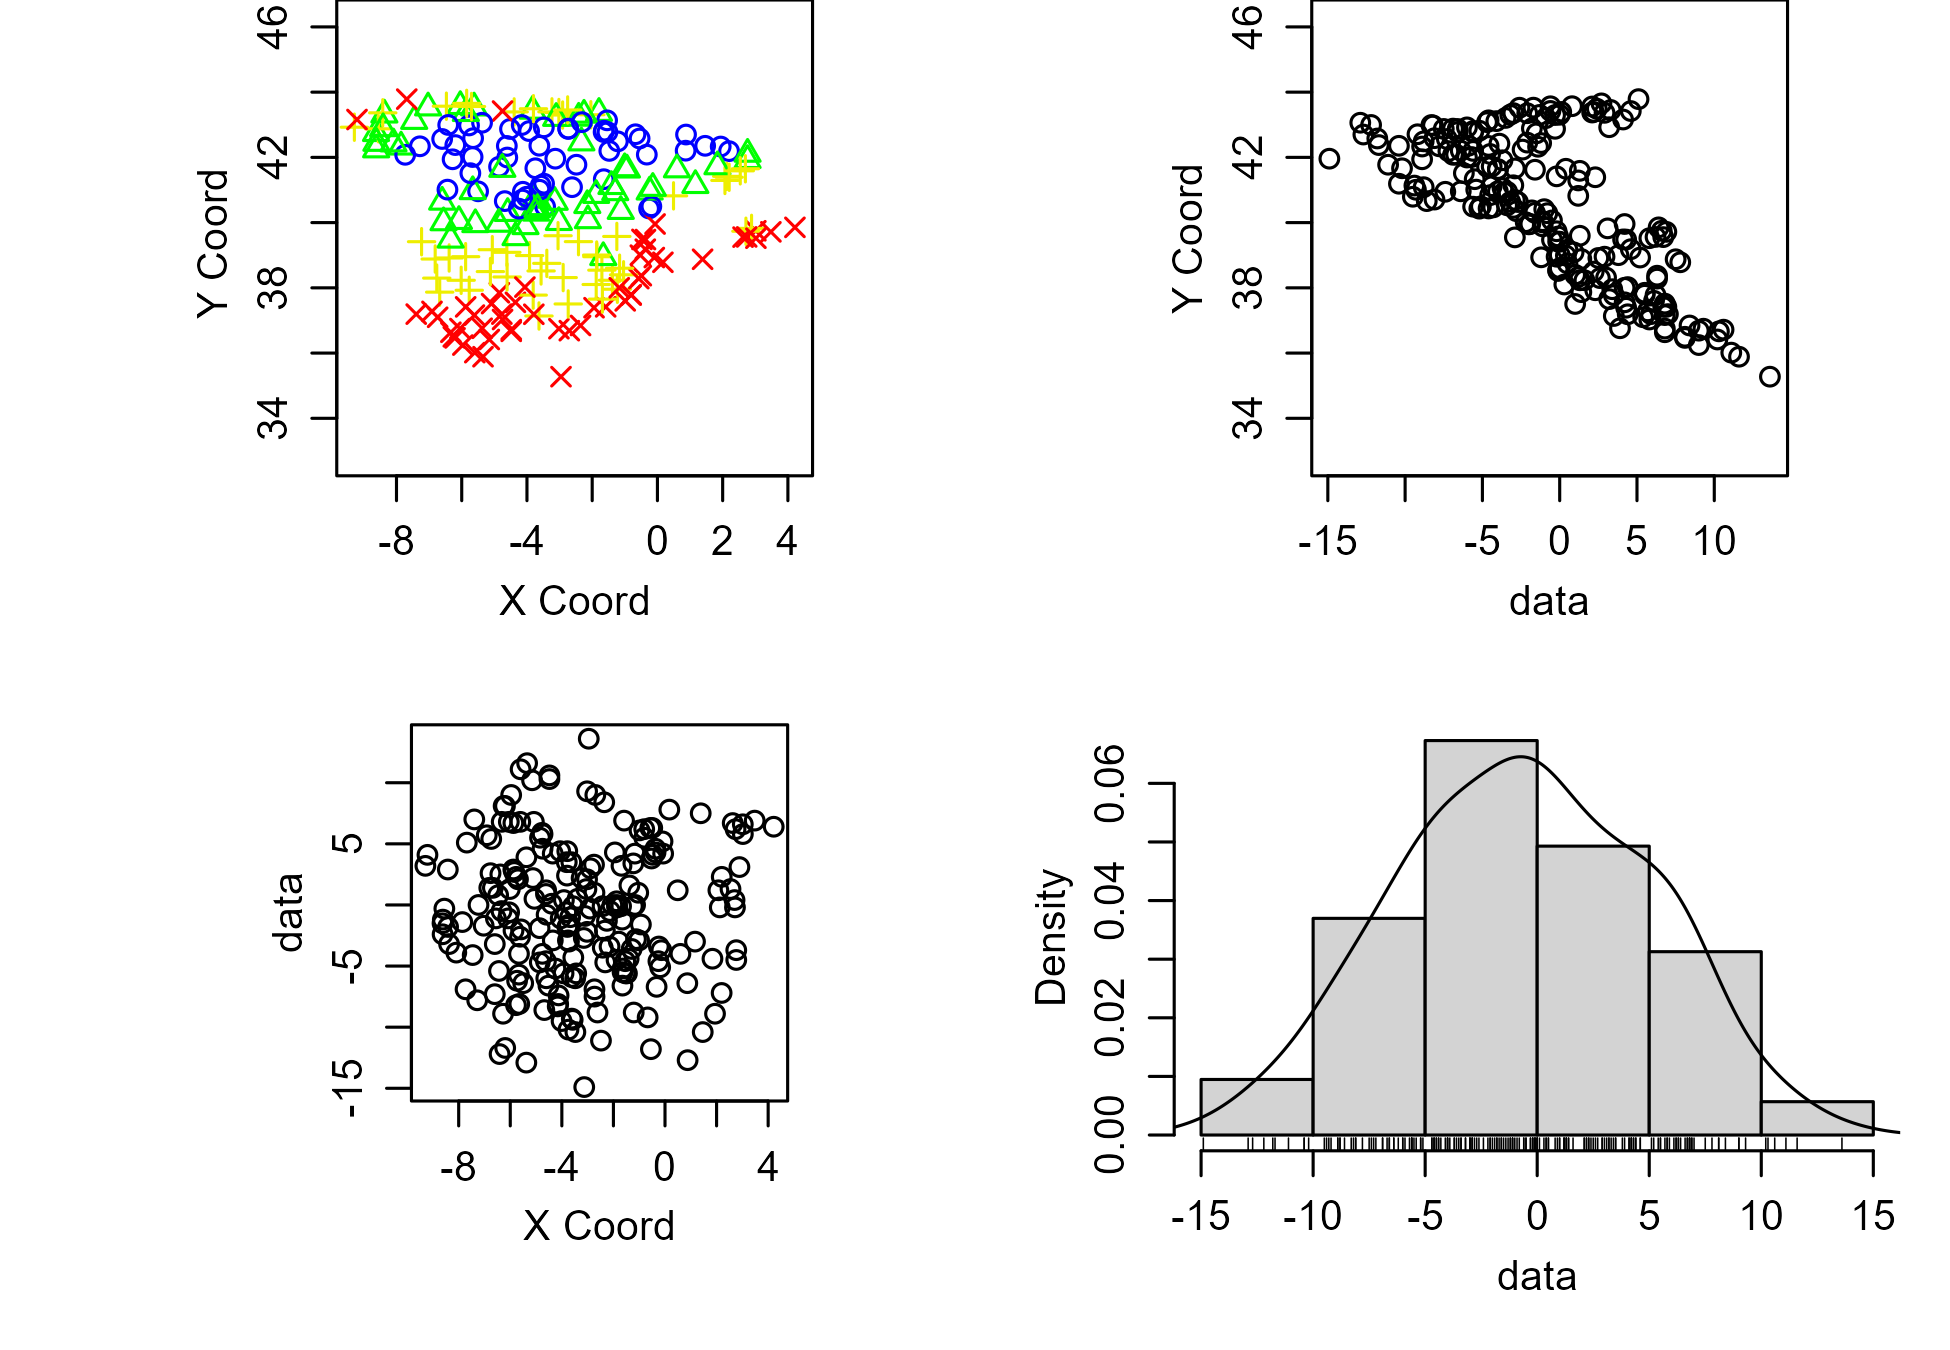
\includegraphics[width=0.6\linewidth]{_main_files/figure-latex/unnamed-chunk-4-1} 

}

\caption{Objetos en geoR}\label{fig:unnamed-chunk-4}
\end{figure}

\emph{Tarea 4. Convertir} \texttt{tmin} \emph{a un objeto de la clase espacial} \texttt{sf}

En esta tarea, convertiremos los datos de tmin en un objeto espacial \texttt{sf}, es
decir, datos espaciales de tipo vector.

Los datos de \texttt{tmin} contienen coordenadas geográficas longitud/latitud, asi que
como vimos en la sección \textbf{Sistema de Referencia de Coordenadas (CRS)} el CRS a
emplear ha de ser un CRS geográfico. Usaremos el código EPSG \textbf{4326}, que
corresponde a coordenadas geográficas y suele ser el habitual en este tipo de
situaciones.

\begin{Shaded}
\begin{Highlighting}[]
\FunctionTok{library}\NormalTok{(sf)}

\NormalTok{tmin\_sf }\OtherTok{\textless{}{-}} \FunctionTok{st\_as\_sf}\NormalTok{(tmin,}
  \AttributeTok{coords =} \FunctionTok{c}\NormalTok{(}\StringTok{"longitud"}\NormalTok{, }\StringTok{"latitud"}\NormalTok{),}
  \AttributeTok{crs =} \DecValTok{4326}
\NormalTok{)}

\NormalTok{tmin\_sf}
\CommentTok{\#\textgreater{} Simple feature collection with 1066 features and 3 fields}
\CommentTok{\#\textgreater{} Geometry type: POINT}
\CommentTok{\#\textgreater{} Dimension:     XY}
\CommentTok{\#\textgreater{} Bounding box:  xmin: {-}9.291389 ymin: 35.27639 xmax: 4.215556 ymax: 43.78611}
\CommentTok{\#\textgreater{} Geodetic CRS:  WGS 84}
\CommentTok{\#\textgreater{} \# A tibble: 1,066 x 4}
\CommentTok{\#\textgreater{}    fecha      indicativo  tmin             geometry}
\CommentTok{\#\textgreater{}  * \textless{}date\textgreater{}     \textless{}chr\textgreater{}      \textless{}dbl\textgreater{}          \textless{}POINT [°]\textgreater{}}
\CommentTok{\#\textgreater{}  1 2021{-}01{-}06 4358X       {-}4.7 ({-}5.880556 38.95556)}
\CommentTok{\#\textgreater{}  2 2021{-}01{-}06 4220X       {-}7   ({-}4.616389 39.08861)}
\CommentTok{\#\textgreater{}  3 2021{-}01{-}06 6106X        4.7 ({-}4.748333 37.02944)}
\CommentTok{\#\textgreater{}  4 2021{-}01{-}06 9698U       {-}6.8  (0.865278 42.20528)}
\CommentTok{\#\textgreater{}  5 2021{-}01{-}06 4410X       {-}3.4 ({-}6.385556 38.91583)}
\CommentTok{\#\textgreater{}  6 2021{-}01{-}06 1331A        1   ({-}7.031389 43.52472)}
\CommentTok{\#\textgreater{}  7 2021{-}01{-}06 1690A       {-}0.1 ({-}7.859722 42.32528)}
\CommentTok{\#\textgreater{}  8 2021{-}01{-}06 8489X       {-}8   ({-}0.255833 40.43333)}
\CommentTok{\#\textgreater{}  9 2021{-}01{-}06 8025         2    ({-}0.494167 38.3725)}
\CommentTok{\#\textgreater{} 10 2021{-}01{-}06 9784P      {-}10       (0.224722 42.63)}
\CommentTok{\#\textgreater{} \# ... with 1,056 more rows}
\end{Highlighting}
\end{Shaded}

\emph{Tarea 5: Dibujemos las estaciones de monitoreo de la temperaria mínima en un
mapa de España. Ámbito espacial.}

Vamos, además, a incluir una capa de las comunidades autónomas de España. Para
ello usaremos un paquete API que nos proporciona esta información en formato
\texttt{sf}:

\begin{Shaded}
\begin{Highlighting}[]
\FunctionTok{library}\NormalTok{(mapSpain)}
\CommentTok{\# sf object}
\NormalTok{esp }\OtherTok{\textless{}{-}} \FunctionTok{esp\_get\_ccaa}\NormalTok{() }\SpecialCharTok{\%\textgreater{}\%}
  \CommentTok{\# No vamos a usar Canarias en este análisis}
  \FunctionTok{filter}\NormalTok{(ine.ccaa.name }\SpecialCharTok{!=} \StringTok{"Canarias"}\NormalTok{)}


\FunctionTok{plot}\NormalTok{(esp}\SpecialCharTok{$}\NormalTok{geometry) }\CommentTok{\# Dibujamo el mapa de España menos las Islas Canarias}
\end{Highlighting}
\end{Shaded}

\begin{figure}

{\centering 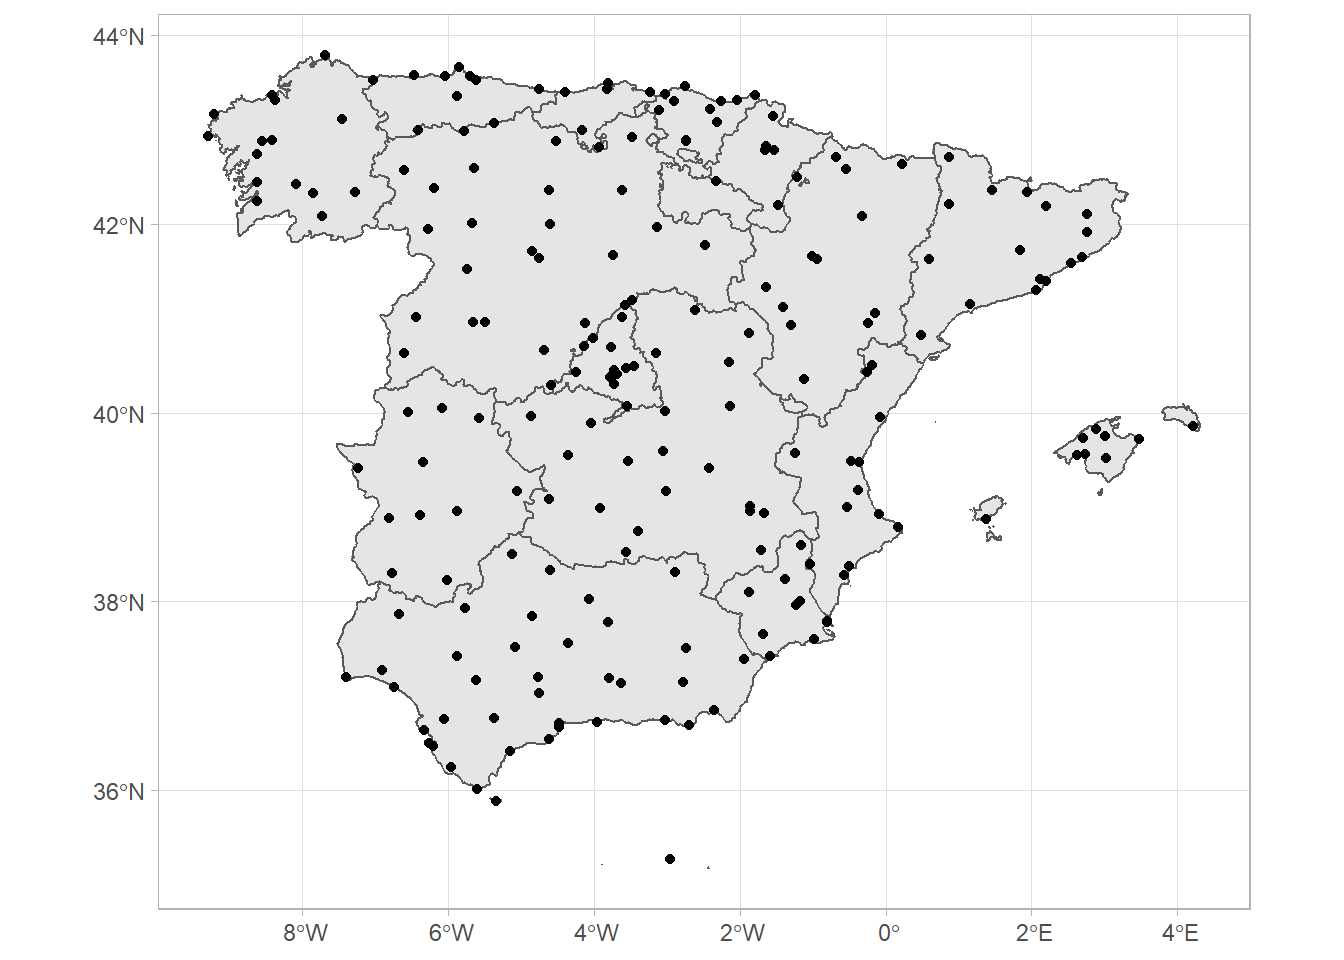
\includegraphics[width=0.6\linewidth]{_main_files/figure-latex/unnamed-chunk-6-1} 

}

\caption{Mapa de España (Sin Canarias)}\label{fig:unnamed-chunk-6}
\end{figure}

\textbf{Q2: ¿Tengo el Sistema de referencia de coordenadas (CRS) de las estaciones de
monitoreo en la misma proyección que el contorno de España?}

Como se comentó en la sección \textbf{Sistema de Referencia de Coordenadas (CRS)},
cuando se emplean datos geográficos provenientes de varias fuentes, es necesario
asegurarse de que ambos objetos están usando el mismo CRS. Vamos a comprobarlo:

\begin{Shaded}
\begin{Highlighting}[]
\FunctionTok{st\_crs}\NormalTok{(tmin\_sf) }\SpecialCharTok{==} \FunctionTok{st\_crs}\NormalTok{(esp)}
\CommentTok{\#\textgreater{} [1] FALSE}
\end{Highlighting}
\end{Shaded}

Vemos que no lo están, por lo que vamos a proyectar las coordenadas a un CRS
común. En este caso usaremos el CRS de referencia de \texttt{tmin\_sf}:

\begin{Shaded}
\begin{Highlighting}[]
\NormalTok{esp2 }\OtherTok{\textless{}{-}} \FunctionTok{st\_transform}\NormalTok{(esp, }\FunctionTok{st\_crs}\NormalTok{(tmin\_sf))}

\FunctionTok{st\_crs}\NormalTok{(tmin\_sf) }\SpecialCharTok{==} \FunctionTok{st\_crs}\NormalTok{(esp2)}
\CommentTok{\#\textgreater{} [1] TRUE}
\end{Highlighting}
\end{Shaded}

Dibujamos las estaciones de monitoreo con el contorno de España. Vamos a usar el
paquete \texttt{ggplot2} como referencia, sin embargo existen varios paquetes
especializados en mapas temáticos, como pueden ser \texttt{tmap} o \texttt{mapsf}.

\begin{Shaded}
\begin{Highlighting}[]
\FunctionTok{library}\NormalTok{(ggplot2)}

\FunctionTok{ggplot}\NormalTok{(esp2) }\SpecialCharTok{+}
  \CommentTok{\# Para graficar objetos sf debemos usar geom\_sf()}
  \FunctionTok{geom\_sf}\NormalTok{() }\SpecialCharTok{+}
  \FunctionTok{geom\_sf}\NormalTok{(}\AttributeTok{data =}\NormalTok{ tmin\_sf) }\SpecialCharTok{+}
  \FunctionTok{theme\_light}\NormalTok{() }\SpecialCharTok{+}
  \FunctionTok{labs}\NormalTok{(}
    \AttributeTok{title =} \StringTok{"Estaciones de monitoreo AEMET en  España"}\NormalTok{,}
    \AttributeTok{subtitle =} \StringTok{"excluyendo las Islas Canarias"}
\NormalTok{  ) }\SpecialCharTok{+}
  \FunctionTok{theme}\NormalTok{(}
    \AttributeTok{plot.title =} \FunctionTok{element\_text}\NormalTok{(}
      \AttributeTok{size =} \DecValTok{12}\NormalTok{,}
      \AttributeTok{face =} \StringTok{"bold"}
\NormalTok{    ),}
    \AttributeTok{plot.subtitle =} \FunctionTok{element\_text}\NormalTok{(}
      \AttributeTok{size =} \DecValTok{8}\NormalTok{,}
      \AttributeTok{face =} \StringTok{"italic"}
\NormalTok{    )}
\NormalTok{  )}
\end{Highlighting}
\end{Shaded}

\begin{figure}

{\centering 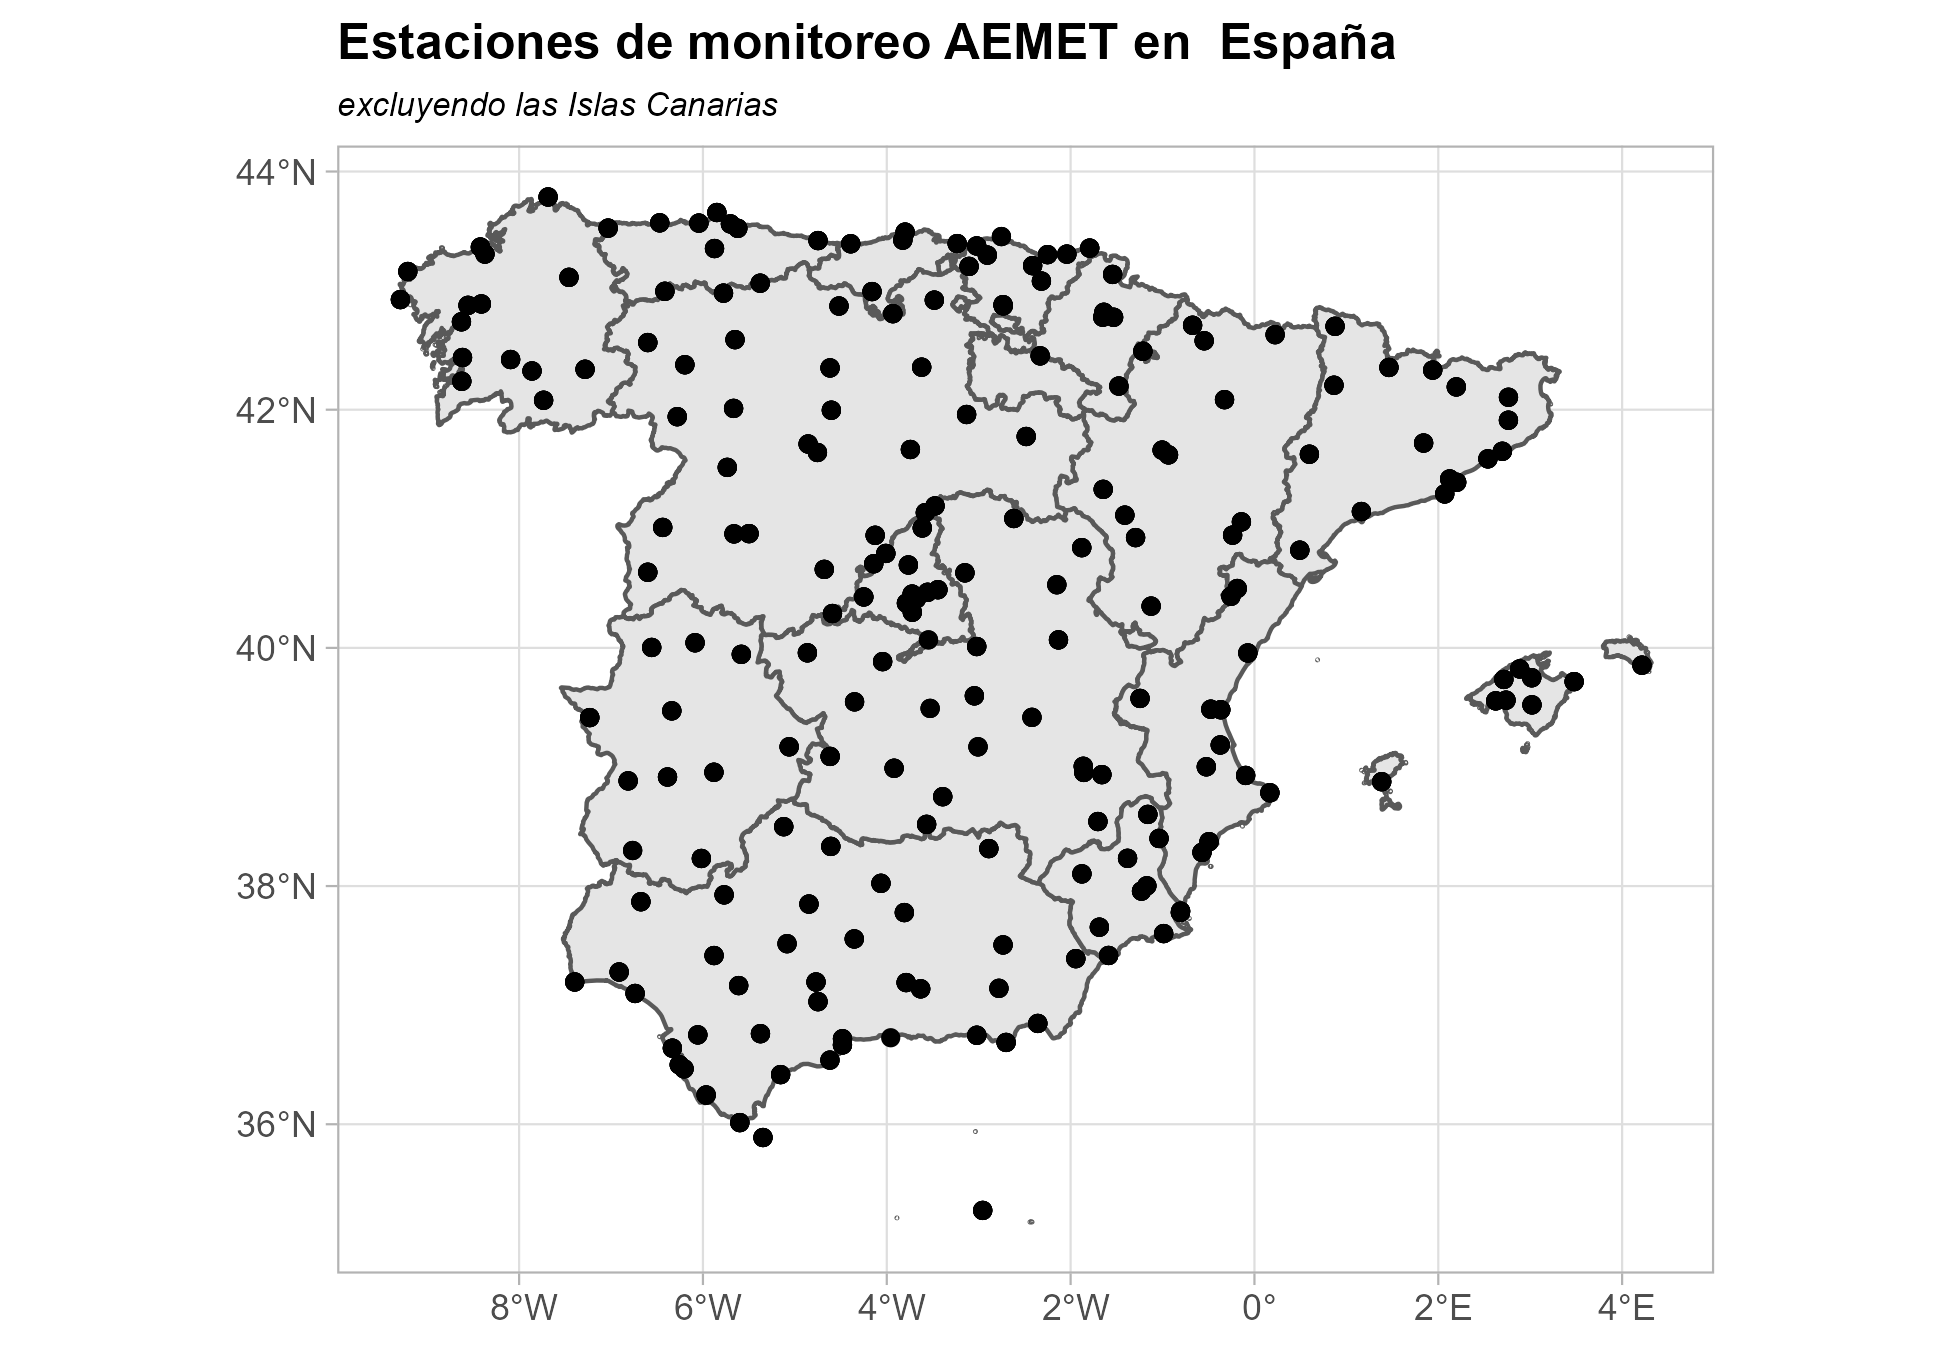
\includegraphics[width=0.6\linewidth]{_main_files/figure-latex/unnamed-chunk-8-1} 

}

\caption{Estaciones de AEMET en la Península Ibérica}\label{fig:unnamed-chunk-8}
\end{figure}

\emph{Tarea 6: Representamos la variable temperatura mínima \texttt{tmin} para el día 8 de
enero de 2021.}

En la siguiente tarea, seleccionaremos los datos correspondientes al \textbf{8 de
enero de 2021} y crearemos un mapa temático en el que representaremos los
valores de temperatura mínima registrados en cada estación mediante un código de
colores.

\begin{Shaded}
\begin{Highlighting}[]
\NormalTok{tmin\_8enero }\OtherTok{\textless{}{-}}\NormalTok{ tmin\_sf }\SpecialCharTok{\%\textgreater{}\%}
  \CommentTok{\# seleccionamos el día y la variable}
  \FunctionTok{filter}\NormalTok{(fecha }\SpecialCharTok{==} \StringTok{"2021{-}01{-}08"}\NormalTok{)}


\FunctionTok{plot}\NormalTok{(tmin\_8enero[}\StringTok{"tmin"}\NormalTok{],}
  \AttributeTok{main =} \StringTok{"Temperatura mínima (8{-}enero{-}2021)"}\NormalTok{,}
  \AttributeTok{pch =} \DecValTok{8}
\NormalTok{)}
\end{Highlighting}
\end{Shaded}

\begin{figure}

{\centering 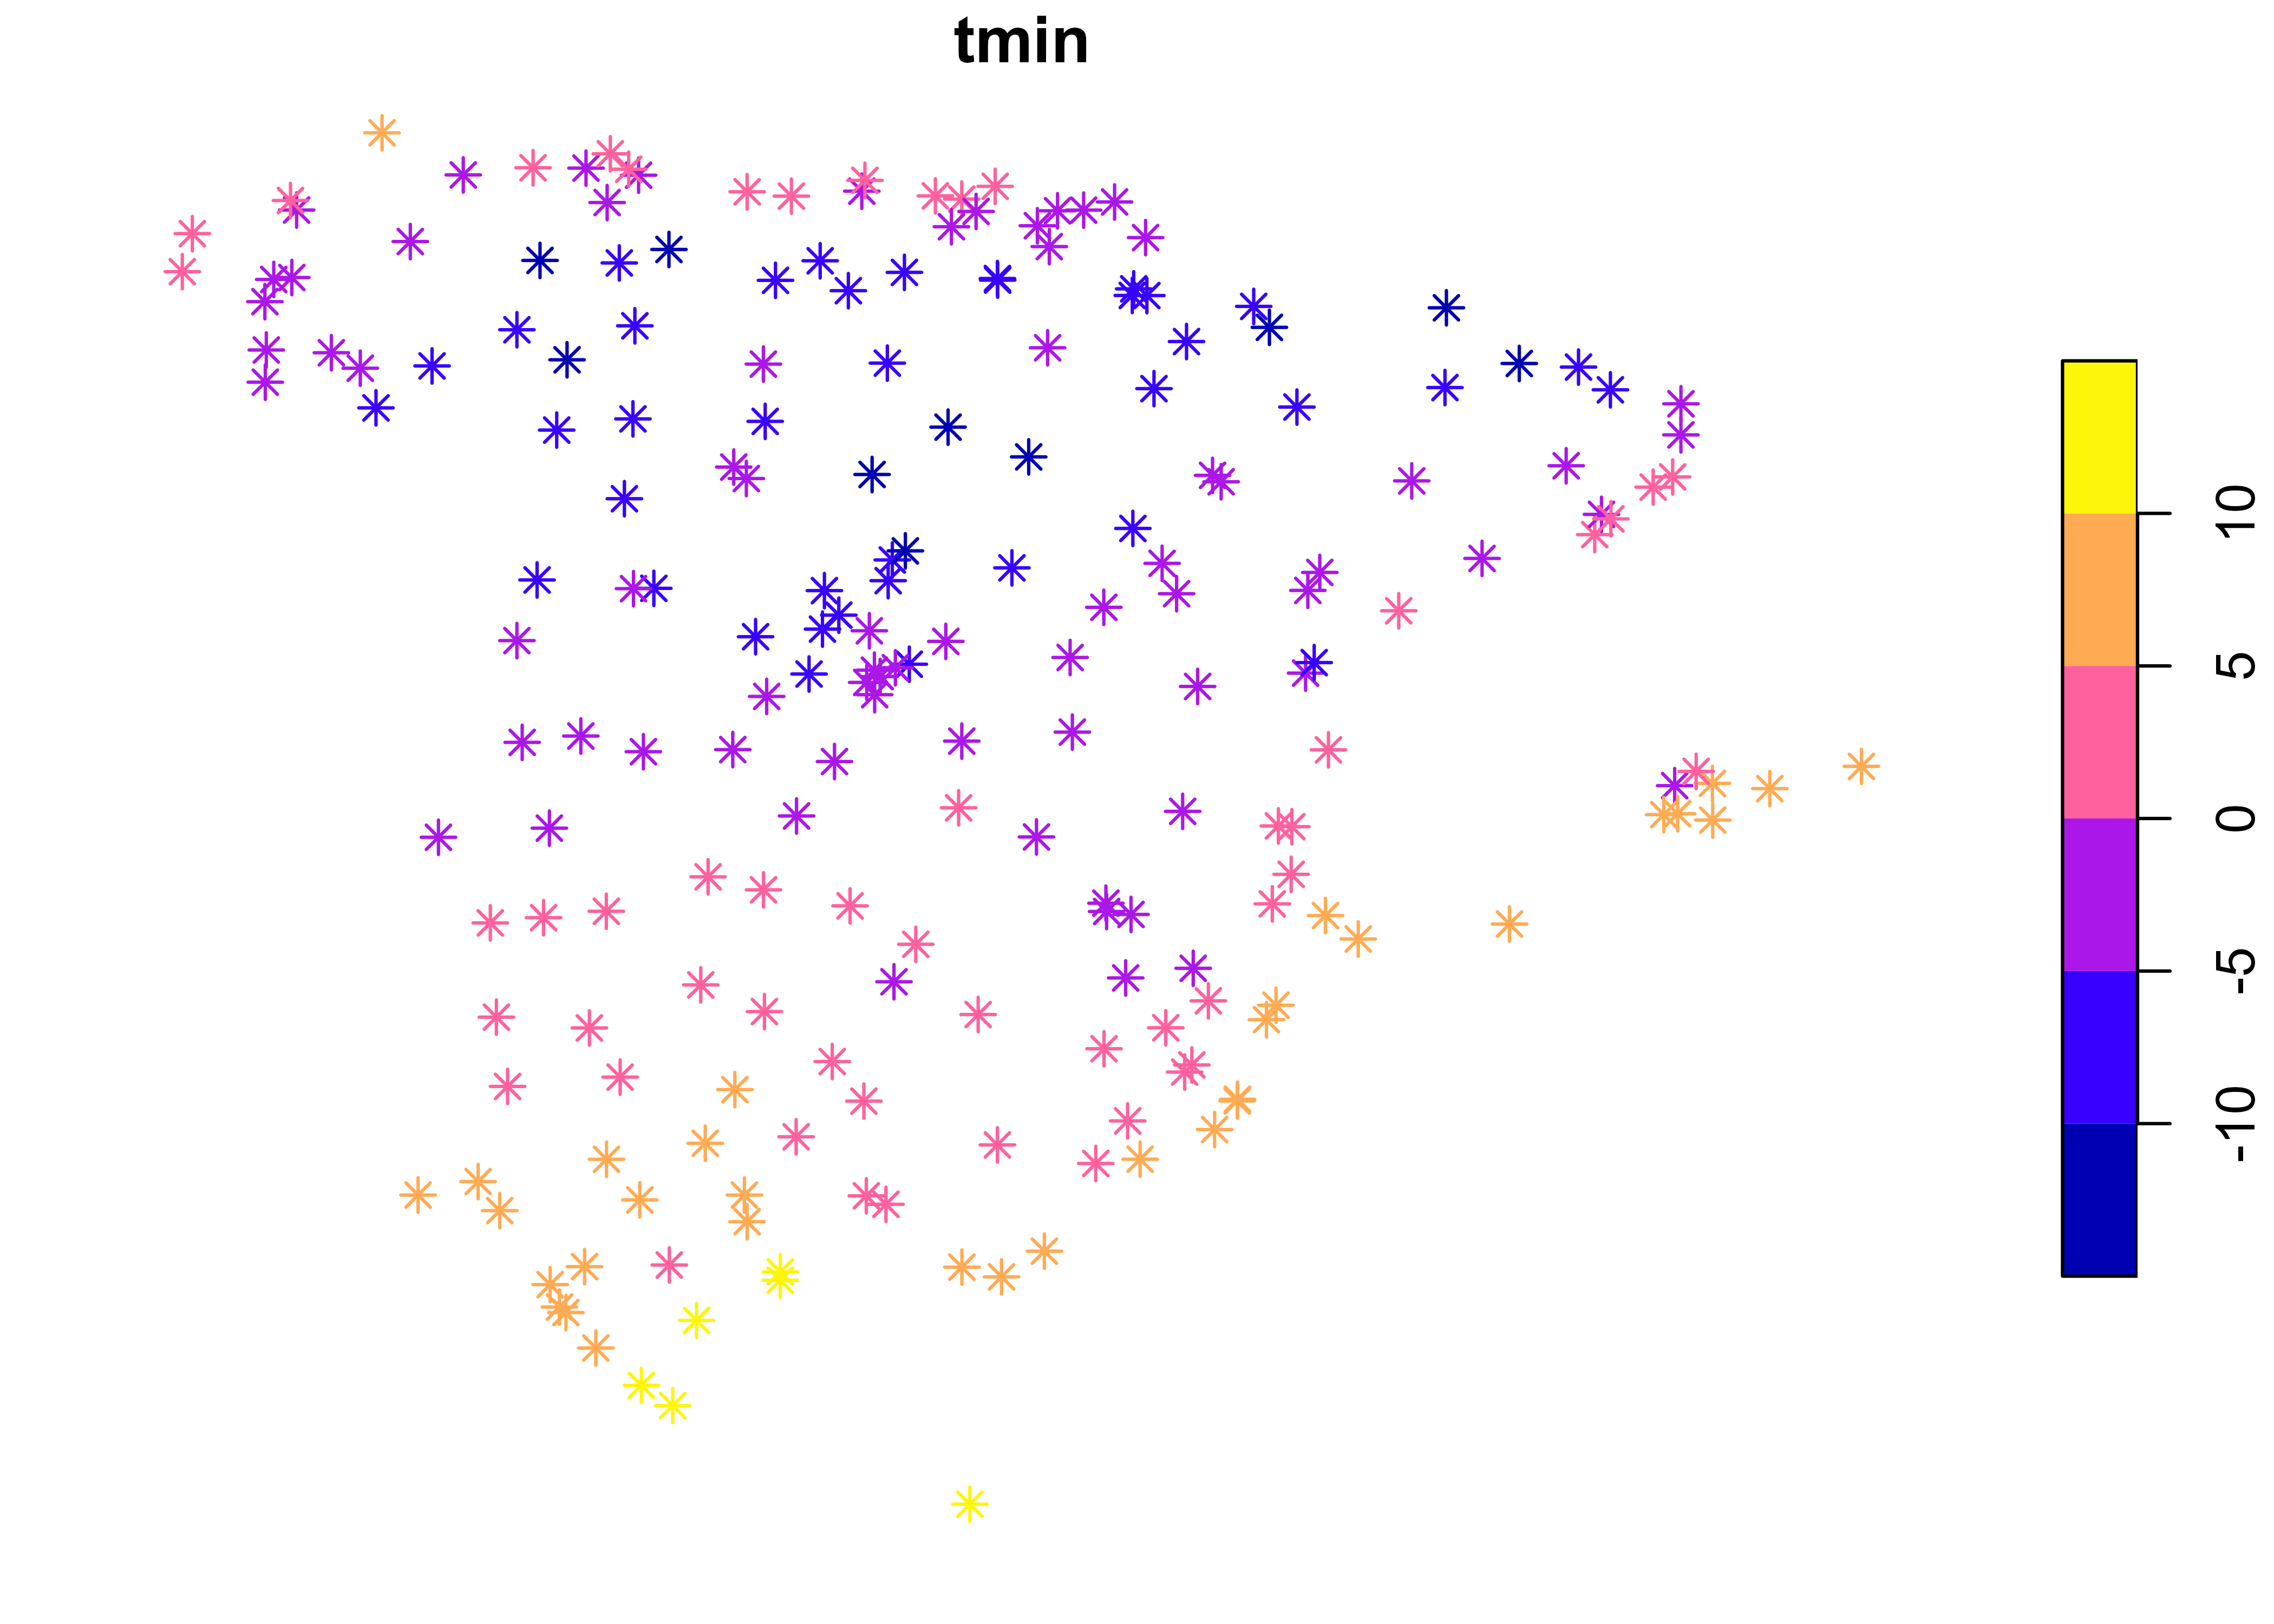
\includegraphics[width=0.6\linewidth]{_main_files/figure-latex/plot-base-tmin-1} 

}

\caption{Mapa de puntos con temperatura mínima}\label{fig:plot-base-tmin}
\end{figure}

Podemos utilizar el ámbito espacial, el contorno de España para graficar y
contar la historia de la Filomena un poco mejor.

\begin{figure}

{\centering 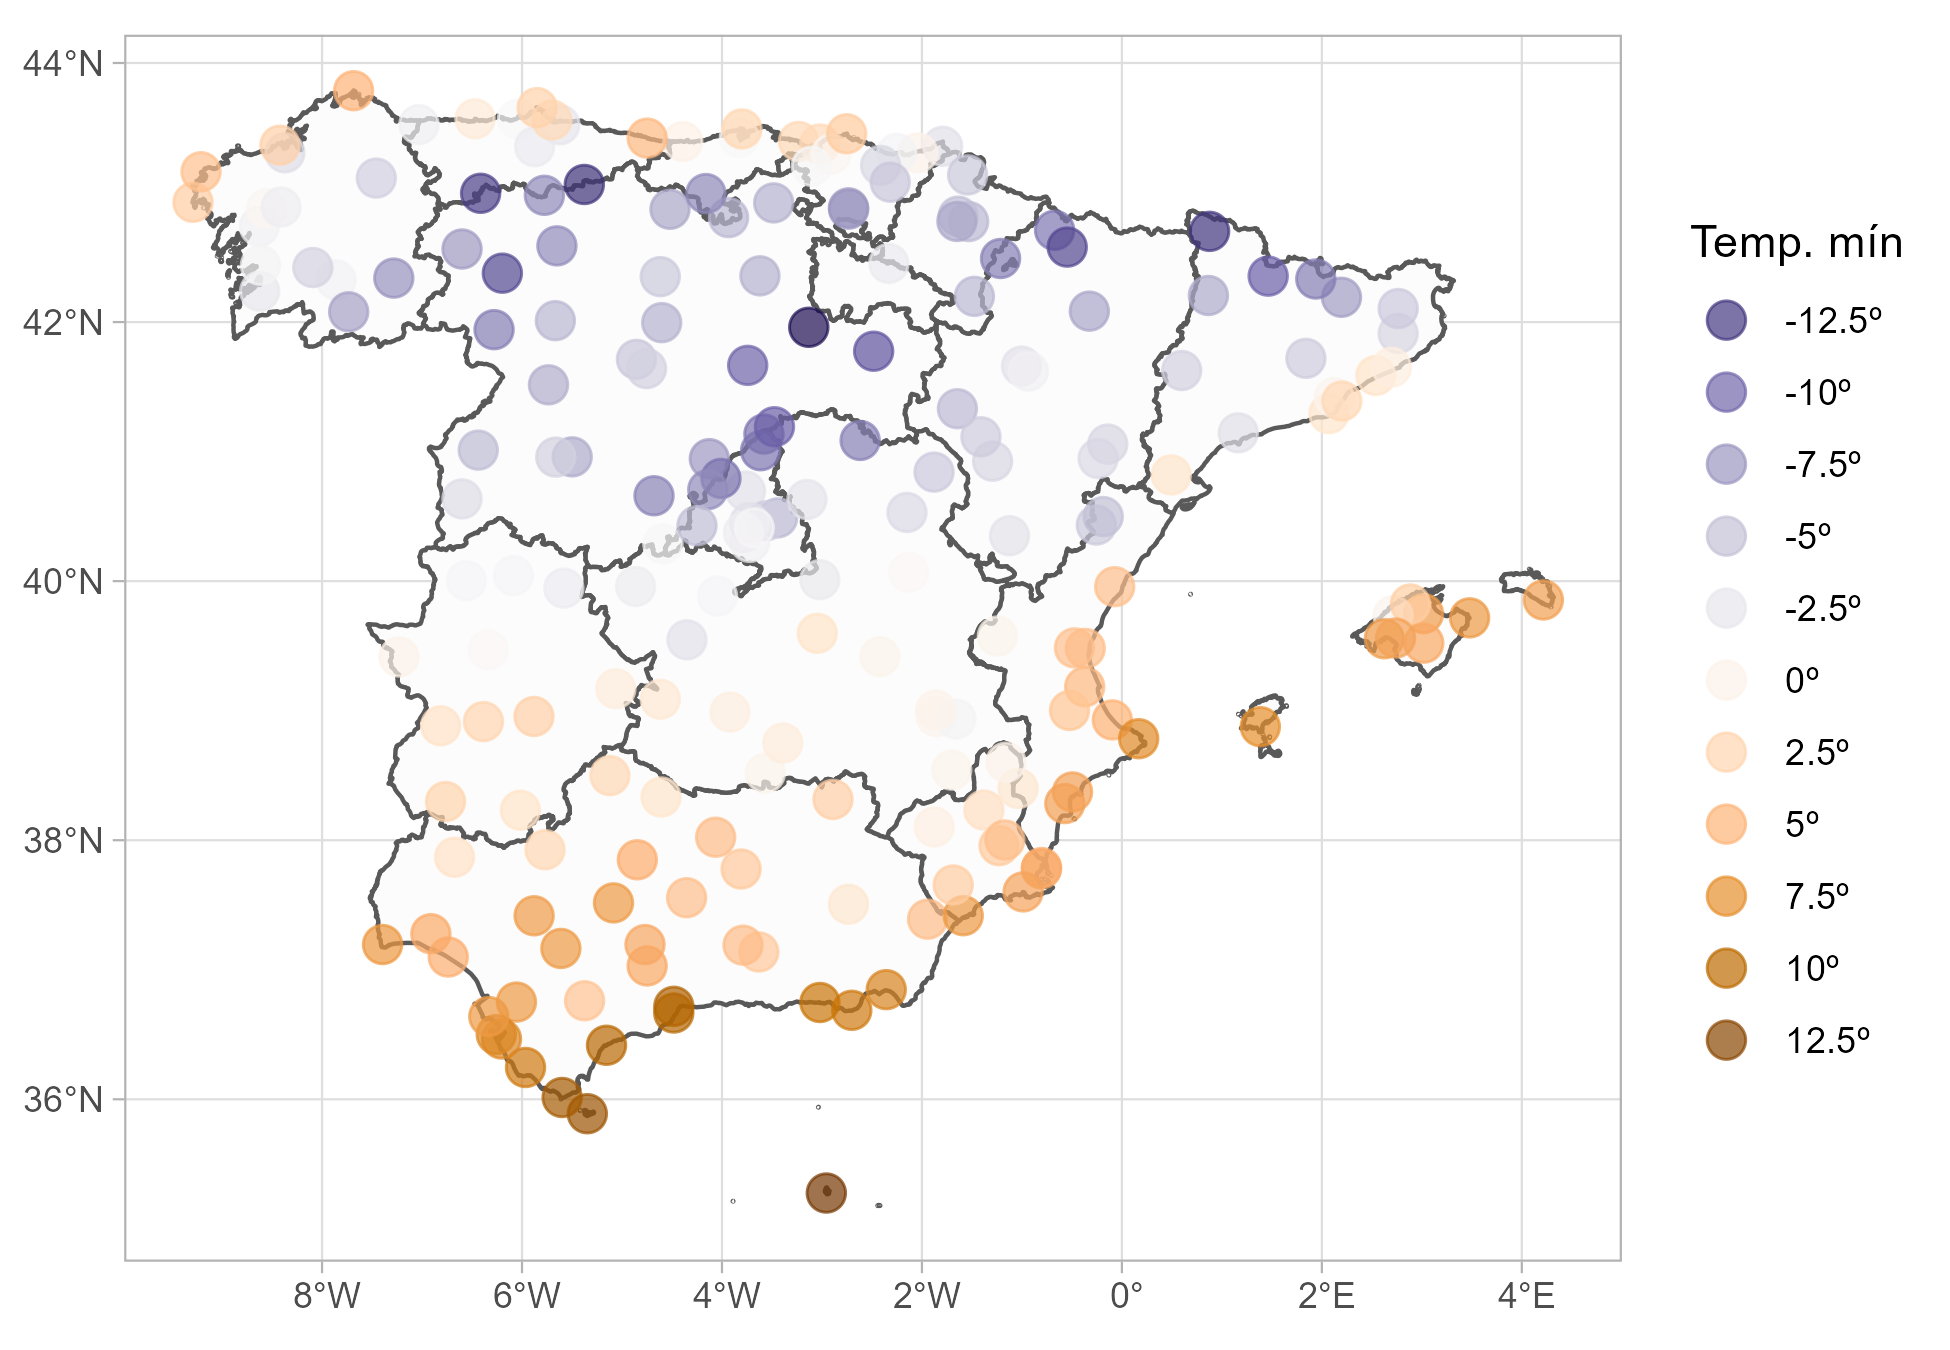
\includegraphics[width=0.6\linewidth]{_main_files/figure-latex/spatial-plots-1} 

}

\caption{Mapa completo con temperatura mínima}\label{fig:spatial-plots}
\end{figure}

\emph{Tarea 7: Interpolación de la variable temperatura mínima \texttt{tmin} para el día 8
de enero de 2021 con IDW}

\textbf{Q3}: El mapa ha quedado muy claro. Vemos como los datos nos cuentan la
historia de Filomena en aquellos sitios donde se tomaron mediciones, pero
\textbf{¿podríamos tener un mapa de interpolación para tener una estimación de la
temperatura mínima en las partes donde la AEMET no tiene estación de
monitoreo?}

Tal y como se avanzó en teoría, parece lógico pensar que aquellos puntos que
estén cerca tendrán valores similares así que tomemos ventaja de la dependencia
espacial y utilicemos un método determinista, como la Distancia Inversa
Ponderada, comúnmente conocido por su acrónimo inglés IDW (Inverse distance
weighted), el cual es uno de los métodos más simples para llevar para llevar a
cabo una interpolación espacial.

En este tipo de análisis, es crucial que el CRS sea el apropiado. En este caso,
ya definimos el CRS como un CRS geográfico (es decir, usando coordenadas de
longitud y latitud). Sin embargo, para el ejercicio de interpolación es más
adecuado usar un CRS local (que provoque pocas deformaciones en la proyección de
España) y en alguna unidad de distancia, como metros (ya vimos que en los CRS
geográficos las unidades son grados).

Si usamos el paquete \texttt{crsuggest} podemos observar los CRS sugeridos:

\begin{Shaded}
\begin{Highlighting}[]
\FunctionTok{library}\NormalTok{(crsuggest)}

\NormalTok{sugiere }\OtherTok{\textless{}{-}} \FunctionTok{suggest\_crs}\NormalTok{(tmin\_8enero, }\AttributeTok{units =} \StringTok{"m"}\NormalTok{, }\AttributeTok{limit =} \DecValTok{5}\NormalTok{)}

\CommentTok{\# Usamos la sugerencia del paquete}
\NormalTok{crs\_sugerido }\OtherTok{\textless{}{-}} \FunctionTok{st\_crs}\NormalTok{(sugiere[}\DecValTok{1}\NormalTok{, ]}\SpecialCharTok{$}\NormalTok{crs\_proj4)}

\NormalTok{esp3 }\OtherTok{\textless{}{-}} \FunctionTok{st\_transform}\NormalTok{(esp2, crs\_sugerido)}
\NormalTok{tmin\_8enero3 }\OtherTok{\textless{}{-}} \FunctionTok{st\_transform}\NormalTok{(tmin\_8enero, crs\_sugerido)}
\end{Highlighting}
\end{Shaded}

\textbf{Q4: ¿Dónde vamos a interpolar? ¿En que puntos?}

Para realizar la interpolación, necesitamos generar una malla que representará
las celdas de las que queremos obtener el valor interpolado.

Dado que hemos proyectado nuestros datos a un CRS cuya unidad son los metros,
podemos definir el tamaño de cada celda en metros cuadrados. En este caso vamos
a usar celdas de 100 kms cuadrados (10 x 10 kms):

\begin{Shaded}
\begin{Highlighting}[]
\FunctionTok{set.seed}\NormalTok{(}\DecValTok{9876}\NormalTok{) }\CommentTok{\# Con esto aseguramos que el grid generado siempre es igual}

\NormalTok{malla\_sf }\OtherTok{\textless{}{-}} \FunctionTok{st\_make\_grid}\NormalTok{(}
\NormalTok{  esp3,}
  \AttributeTok{cellsize =} \DecValTok{8000}
\NormalTok{)}
\end{Highlighting}
\end{Shaded}

Graficamos la superficie para ver exactamente qué hemos construido:

\begin{Shaded}
\begin{Highlighting}[]

\FunctionTok{ggplot}\NormalTok{(esp3) }\SpecialCharTok{+}
  \FunctionTok{geom\_sf}\NormalTok{() }\SpecialCharTok{+}
  \FunctionTok{geom\_sf}\NormalTok{(}
    \AttributeTok{data =}\NormalTok{ malla\_sf,}
    \AttributeTok{size =} \FloatTok{0.1}\NormalTok{,}
    \AttributeTok{col =} \StringTok{"red"}\NormalTok{, }\AttributeTok{alpha =} \DecValTok{1}\NormalTok{,}
    \AttributeTok{fill =} \ConstantTok{NA}
\NormalTok{  ) }\SpecialCharTok{+}
  \FunctionTok{geom\_sf}\NormalTok{(}
    \AttributeTok{data =}\NormalTok{ tmin\_8enero3,}
    \FunctionTok{aes}\NormalTok{(}\AttributeTok{fill =} \StringTok{"AEMET Stations"}\NormalTok{), }\AttributeTok{size =} \DecValTok{4}\NormalTok{, }\AttributeTok{shape =} \DecValTok{21}\NormalTok{,}
    \AttributeTok{color =} \StringTok{"blue"}
\NormalTok{  ) }\SpecialCharTok{+}
  \FunctionTok{scale\_fill\_manual}\NormalTok{(}\AttributeTok{values =} \FunctionTok{adjustcolor}\NormalTok{(}\StringTok{"blue"}\NormalTok{, }\AttributeTok{alpha.f =} \FloatTok{0.2}\NormalTok{)) }\SpecialCharTok{+}
  \FunctionTok{theme\_void}\NormalTok{() }\SpecialCharTok{+}
  \FunctionTok{theme}\NormalTok{(}\AttributeTok{legend.position =} \StringTok{"bottom"}\NormalTok{) }\SpecialCharTok{+}
  \FunctionTok{labs}\NormalTok{(}
    \AttributeTok{title =} \StringTok{"Cuadrícula espacial para interpolar"}\NormalTok{,}
    \AttributeTok{fill =} \StringTok{""}
\NormalTok{  )}
\end{Highlighting}
\end{Shaded}

\begin{figure}

{\centering 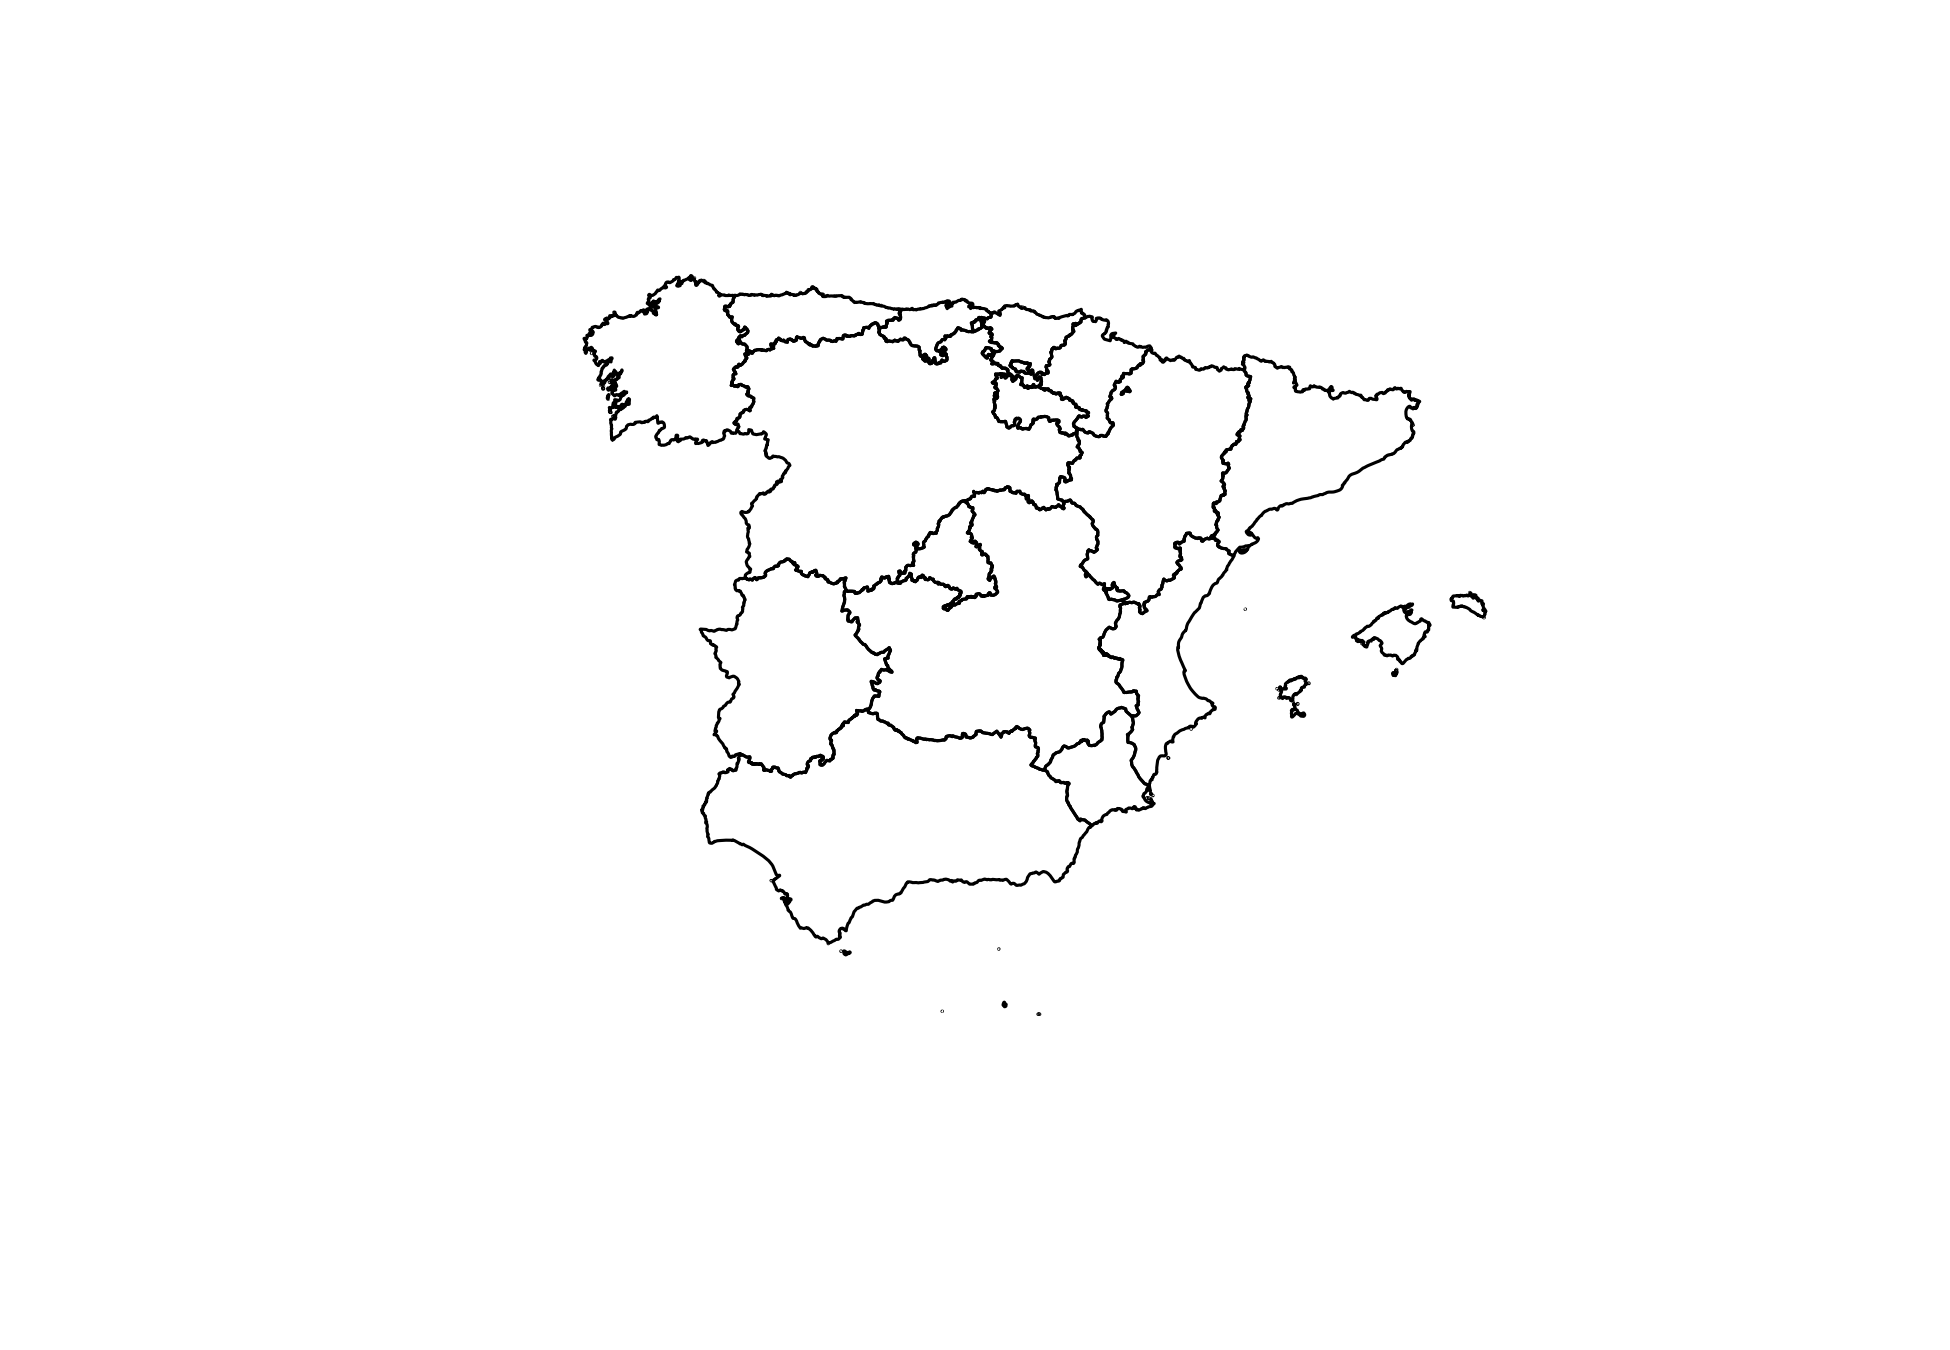
\includegraphics[width=0.6\linewidth]{_main_files/figure-latex/unnamed-chunk-10-1} 

}

\caption{Malla de puntos para interpolación}\label{fig:unnamed-chunk-10}
\end{figure}

Se puede observar claramente cada una de las celdas que hemos creado. La
interpolación asignará un valor a cada uno de ellas.

A continuación podemos llevar a cabo la interpolación usando el paquete \texttt{gstat}.
Además, en lugar de celdas (polígonos) es necesario usar puntos en la
interpolación. Calcularemos, por tanto, un punto representativo de cada celda,
el centroide, que es el punto resultante de realizar la media arimética de las
coordenadas de loss puntos que componen los lados de cada celda

\begin{Shaded}
\begin{Highlighting}[]
\CommentTok{\# Calculamos centroide}
\NormalTok{malla\_sf\_cent }\OtherTok{\textless{}{-}} \FunctionTok{st\_centroid}\NormalTok{(malla\_sf, }\AttributeTok{of\_largest\_polygon =} \ConstantTok{TRUE}\NormalTok{)}

\FunctionTok{library}\NormalTok{(gstat)}
\NormalTok{tmin\_idw }\OtherTok{\textless{}{-}} \FunctionTok{idw}\NormalTok{(}
  \CommentTok{\# Indicamos la variable que queremos interpolar}
\NormalTok{  tmin }\SpecialCharTok{\textasciitilde{}} \DecValTok{1}\NormalTok{,}
  \CommentTok{\# Indicamos el conjunto de datos donde está la variable}
\NormalTok{  tmin\_8enero3,}
  \CommentTok{\# Indicamos la malla de destino, en sf}
  \AttributeTok{newdata =}\NormalTok{ malla\_sf\_cent,}
  \AttributeTok{idp =} \FloatTok{2.0} \CommentTok{\# Especifica la potencia de la IDW}
\NormalTok{)}
\CommentTok{\#\textgreater{} [inverse distance weighted interpolation]}
\FunctionTok{head}\NormalTok{(tmin\_idw)}
\CommentTok{\#\textgreater{} Simple feature collection with 6 features and 2 fields}
\CommentTok{\#\textgreater{} Geometry type: POINT}
\CommentTok{\#\textgreater{} Dimension:     XY}
\CommentTok{\#\textgreater{} Bounding box:  xmin: 146290.9 ymin: 69457.31 xmax: 186290.9 ymax: 69457.31}
\CommentTok{\#\textgreater{} CRS:           +proj=lcc +lat\_1=40 +lat\_0=40 +lon\_0=0 +k\_0=0.9988085293 +x\_0=600000 +y\_0=600000 +a=6378298.3 +rf=294.73 +pm=madrid +units=m +no\_defs}
\CommentTok{\#\textgreater{}   var1.pred var1.var                  geometry}
\CommentTok{\#\textgreater{} 1  2.518621       NA POINT (146290.9 69457.31)}
\CommentTok{\#\textgreater{} 2  2.586930       NA POINT (154290.9 69457.31)}
\CommentTok{\#\textgreater{} 3  2.656846       NA POINT (162290.9 69457.31)}
\CommentTok{\#\textgreater{} 4  2.728395       NA POINT (170290.9 69457.31)}
\CommentTok{\#\textgreater{} 5  2.801600       NA POINT (178290.9 69457.31)}
\CommentTok{\#\textgreater{} 6  2.876486       NA POINT (186290.9 69457.31)}
\end{Highlighting}
\end{Shaded}

\emph{Tarea 8. Mapa de contorno}

Representamos la interpolación con un mapa y mapa de contorno muy utilizado para
representar datos espaciales. Para ello, vamos a usar el paquete \texttt{raster}
convirtiendo nuestro objeto interpolado.

\begin{Shaded}
\begin{Highlighting}[]
\CommentTok{\# Convertimos de sf a SpatiaPixels}
\CommentTok{\# Esto funciona porque nuestros puntos sf están espaciados regularmente}

\NormalTok{tmin\_pixels }\OtherTok{\textless{}{-}}\NormalTok{ tmin\_idw }\SpecialCharTok{\%\textgreater{}\%}
  \FunctionTok{as}\NormalTok{(}\StringTok{"Spatial"}\NormalTok{) }\SpecialCharTok{\%\textgreater{}\%}
  \FunctionTok{as}\NormalTok{(}\StringTok{"SpatialPixels"}\NormalTok{)}


\FunctionTok{library}\NormalTok{(raster)}
\CommentTok{\# Creamos un raster de nuestros pixels}
\NormalTok{rast\_esp }\OtherTok{\textless{}{-}} \FunctionTok{raster}\NormalTok{(tmin\_pixels)}

\CommentTok{\# Transferimos valores del objeto sf al raster}
\NormalTok{rast\_esp2 }\OtherTok{\textless{}{-}} \FunctionTok{rasterize}\NormalTok{(}
\NormalTok{  tmin\_idw,}
\NormalTok{  rast\_esp,}
  \AttributeTok{field =} \StringTok{"var1.pred"}\NormalTok{, }\DocumentationTok{\#\# valores de predicción}
  \AttributeTok{fun =}\NormalTok{ mean}
\NormalTok{)}

\CommentTok{\# Además, podemos recortar el raster a la forma de España}

\NormalTok{rast\_esp\_mask }\OtherTok{\textless{}{-}} \FunctionTok{mask}\NormalTok{(rast\_esp2, esp3)}

\FunctionTok{plot}\NormalTok{(rast\_esp\_mask, }\AttributeTok{col =}\NormalTok{ colores)}
\FunctionTok{contour}\NormalTok{(rast\_esp2, }\AttributeTok{add =} \ConstantTok{TRUE}\NormalTok{)}
\end{Highlighting}
\end{Shaded}

\begin{figure}

{\centering 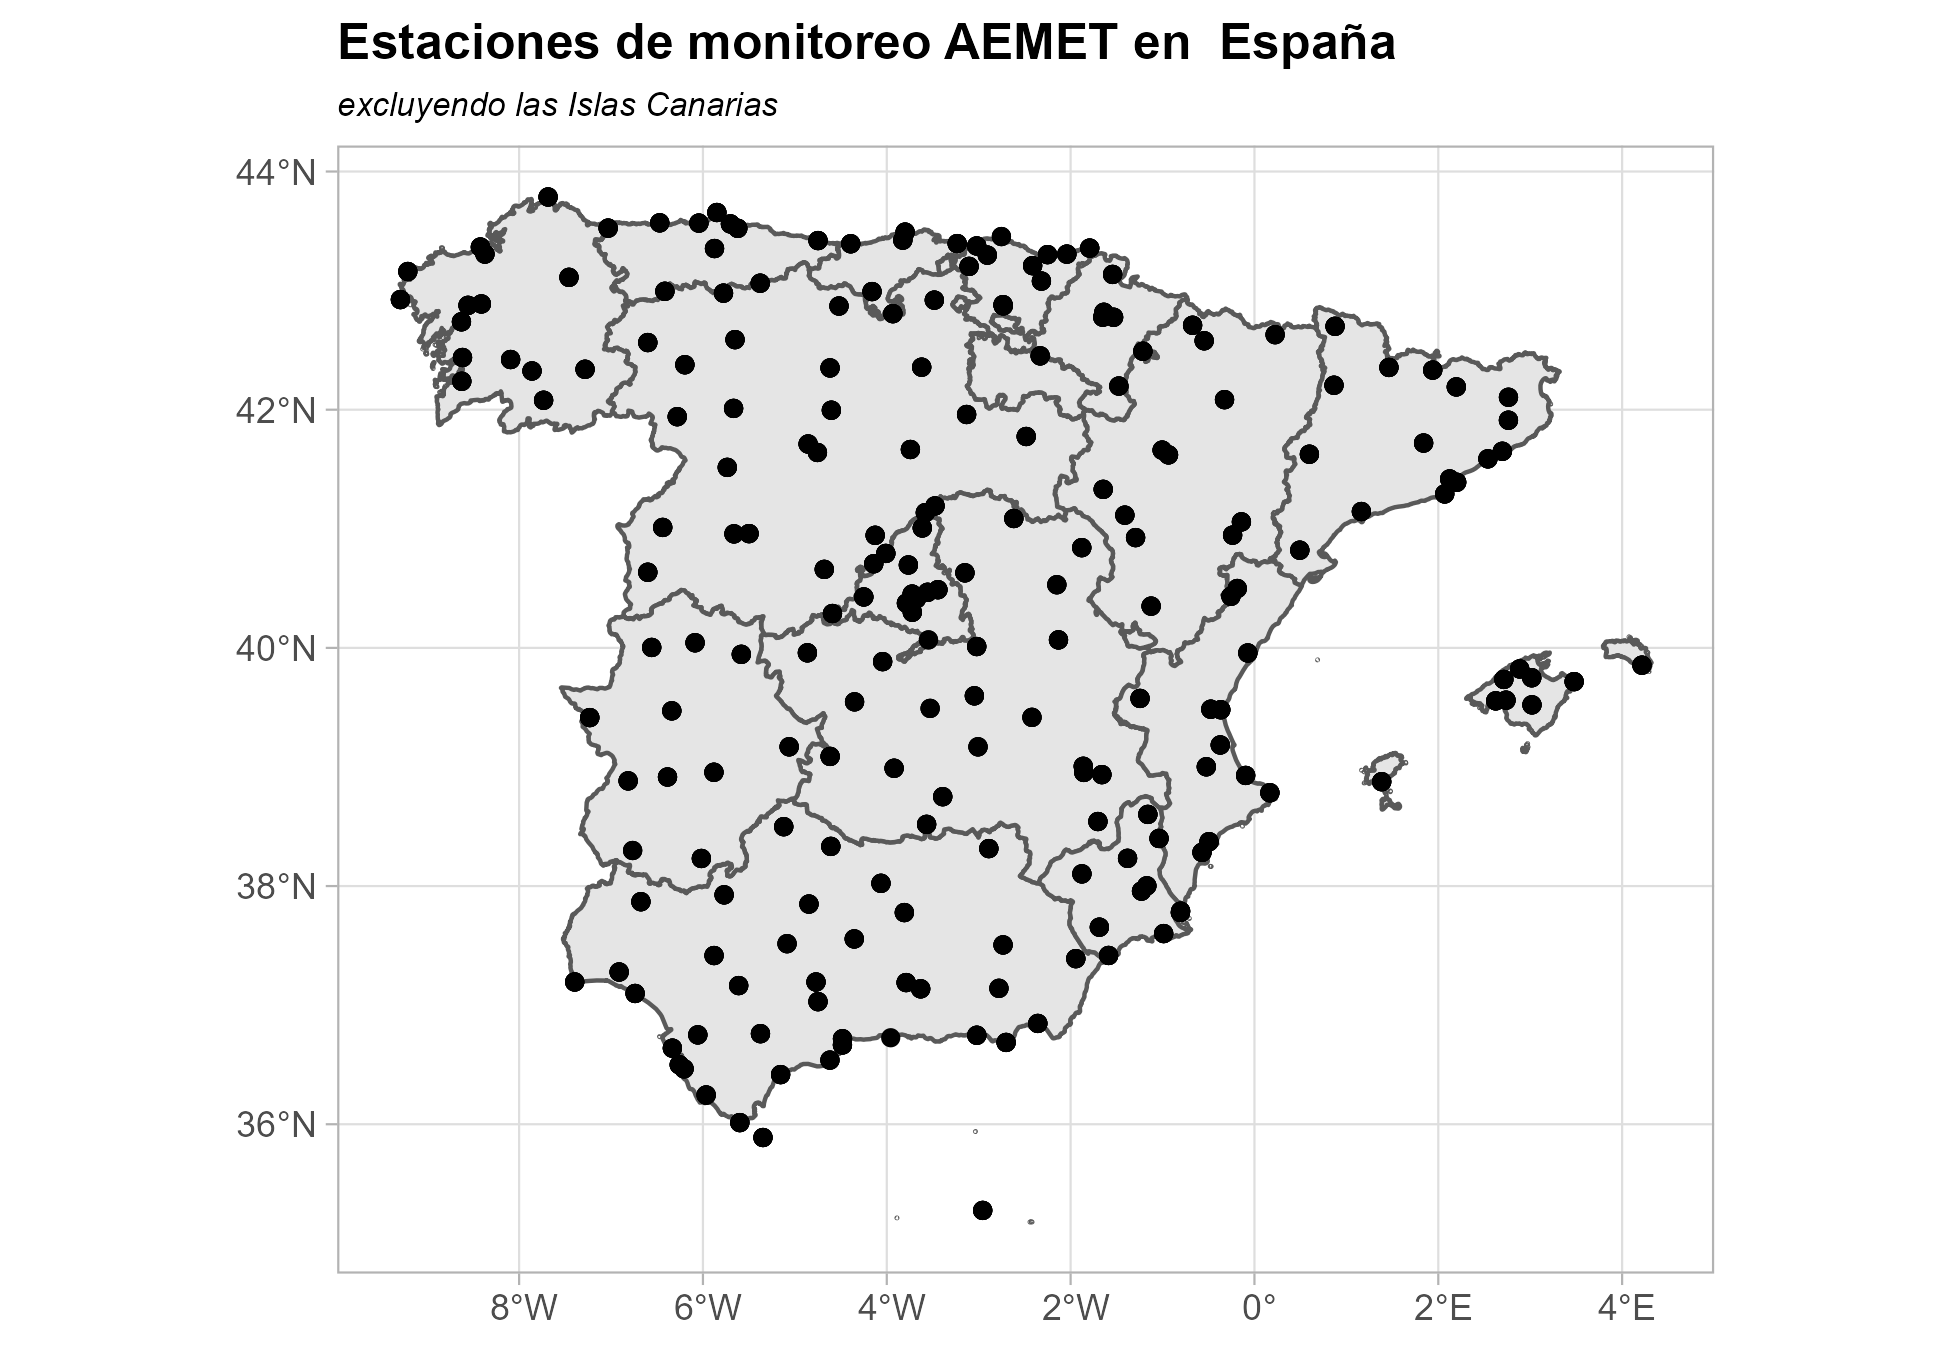
\includegraphics[width=0.6\linewidth]{_main_files/figure-latex/unnamed-chunk-12-1} 

}

\caption{Mapa raster con lineas de nivel}\label{fig:unnamed-chunk-12}
\end{figure}

Podemos realizar el mismo mapa usando \texttt{ggplot2} y la función
\texttt{geom\_contour\_filled}:

\begin{Shaded}
\begin{Highlighting}[]

\CommentTok{\# Creo una tabla para geom contour}
\NormalTok{coordenadas }\OtherTok{\textless{}{-}} \FunctionTok{st\_coordinates}\NormalTok{(tmin\_idw)}
\NormalTok{valor }\OtherTok{\textless{}{-}}\NormalTok{ tmin\_idw}\SpecialCharTok{$}\NormalTok{var1.pred}

\NormalTok{idw\_df }\OtherTok{\textless{}{-}} \FunctionTok{data.frame}\NormalTok{(}
  \CommentTok{\# Necesitamos redondear las coordenadas}
  \AttributeTok{latitud =} \FunctionTok{round}\NormalTok{(coordenadas[, }\DecValTok{2}\NormalTok{], }\DecValTok{6}\NormalTok{),}
  \AttributeTok{longitud =} \FunctionTok{round}\NormalTok{(coordenadas[, }\DecValTok{1}\NormalTok{], }\DecValTok{6}\NormalTok{),}
  \AttributeTok{tmin =}\NormalTok{ valor}
\NormalTok{)}

\FunctionTok{ggplot}\NormalTok{() }\SpecialCharTok{+}
  \FunctionTok{geom\_contour\_filled}\NormalTok{(}
    \AttributeTok{data =}\NormalTok{ idw\_df,}
    \FunctionTok{aes}\NormalTok{(}\AttributeTok{x =}\NormalTok{ longitud, }\AttributeTok{y =}\NormalTok{ latitud, }\AttributeTok{z =}\NormalTok{ tmin),}
    \AttributeTok{na.rm =} \ConstantTok{TRUE}\NormalTok{,}
    \AttributeTok{breaks =}\NormalTok{ cortes}
\NormalTok{  ) }\SpecialCharTok{+}
  \CommentTok{\# Reajustamos la escala de colores}
  \FunctionTok{scale\_fill\_manual}\NormalTok{(}\AttributeTok{values =}\NormalTok{ colores) }\SpecialCharTok{+}
  \CommentTok{\# CCAA}
  \FunctionTok{geom\_sf}\NormalTok{(}\AttributeTok{data =}\NormalTok{ esp3, }\AttributeTok{fill =} \ConstantTok{NA}\NormalTok{) }\SpecialCharTok{+}
  \FunctionTok{theme\_minimal}\NormalTok{() }\SpecialCharTok{+}
  \FunctionTok{theme}\NormalTok{(}\AttributeTok{axis.title =} \FunctionTok{element\_blank}\NormalTok{()) }\SpecialCharTok{+}
  \FunctionTok{labs}\NormalTok{(}
    \AttributeTok{fill =} \StringTok{"Temp. (º)"}\NormalTok{,}
    \AttributeTok{title =} \StringTok{"Temperatura mínima interpolada"}\NormalTok{,}
    \AttributeTok{subtitle =} \StringTok{"8 de Enero 2021"}\NormalTok{,}
    \AttributeTok{caption =} \StringTok{"Datos: AEMET"}
\NormalTok{  )}
\end{Highlighting}
\end{Shaded}

\begin{figure}

{\centering 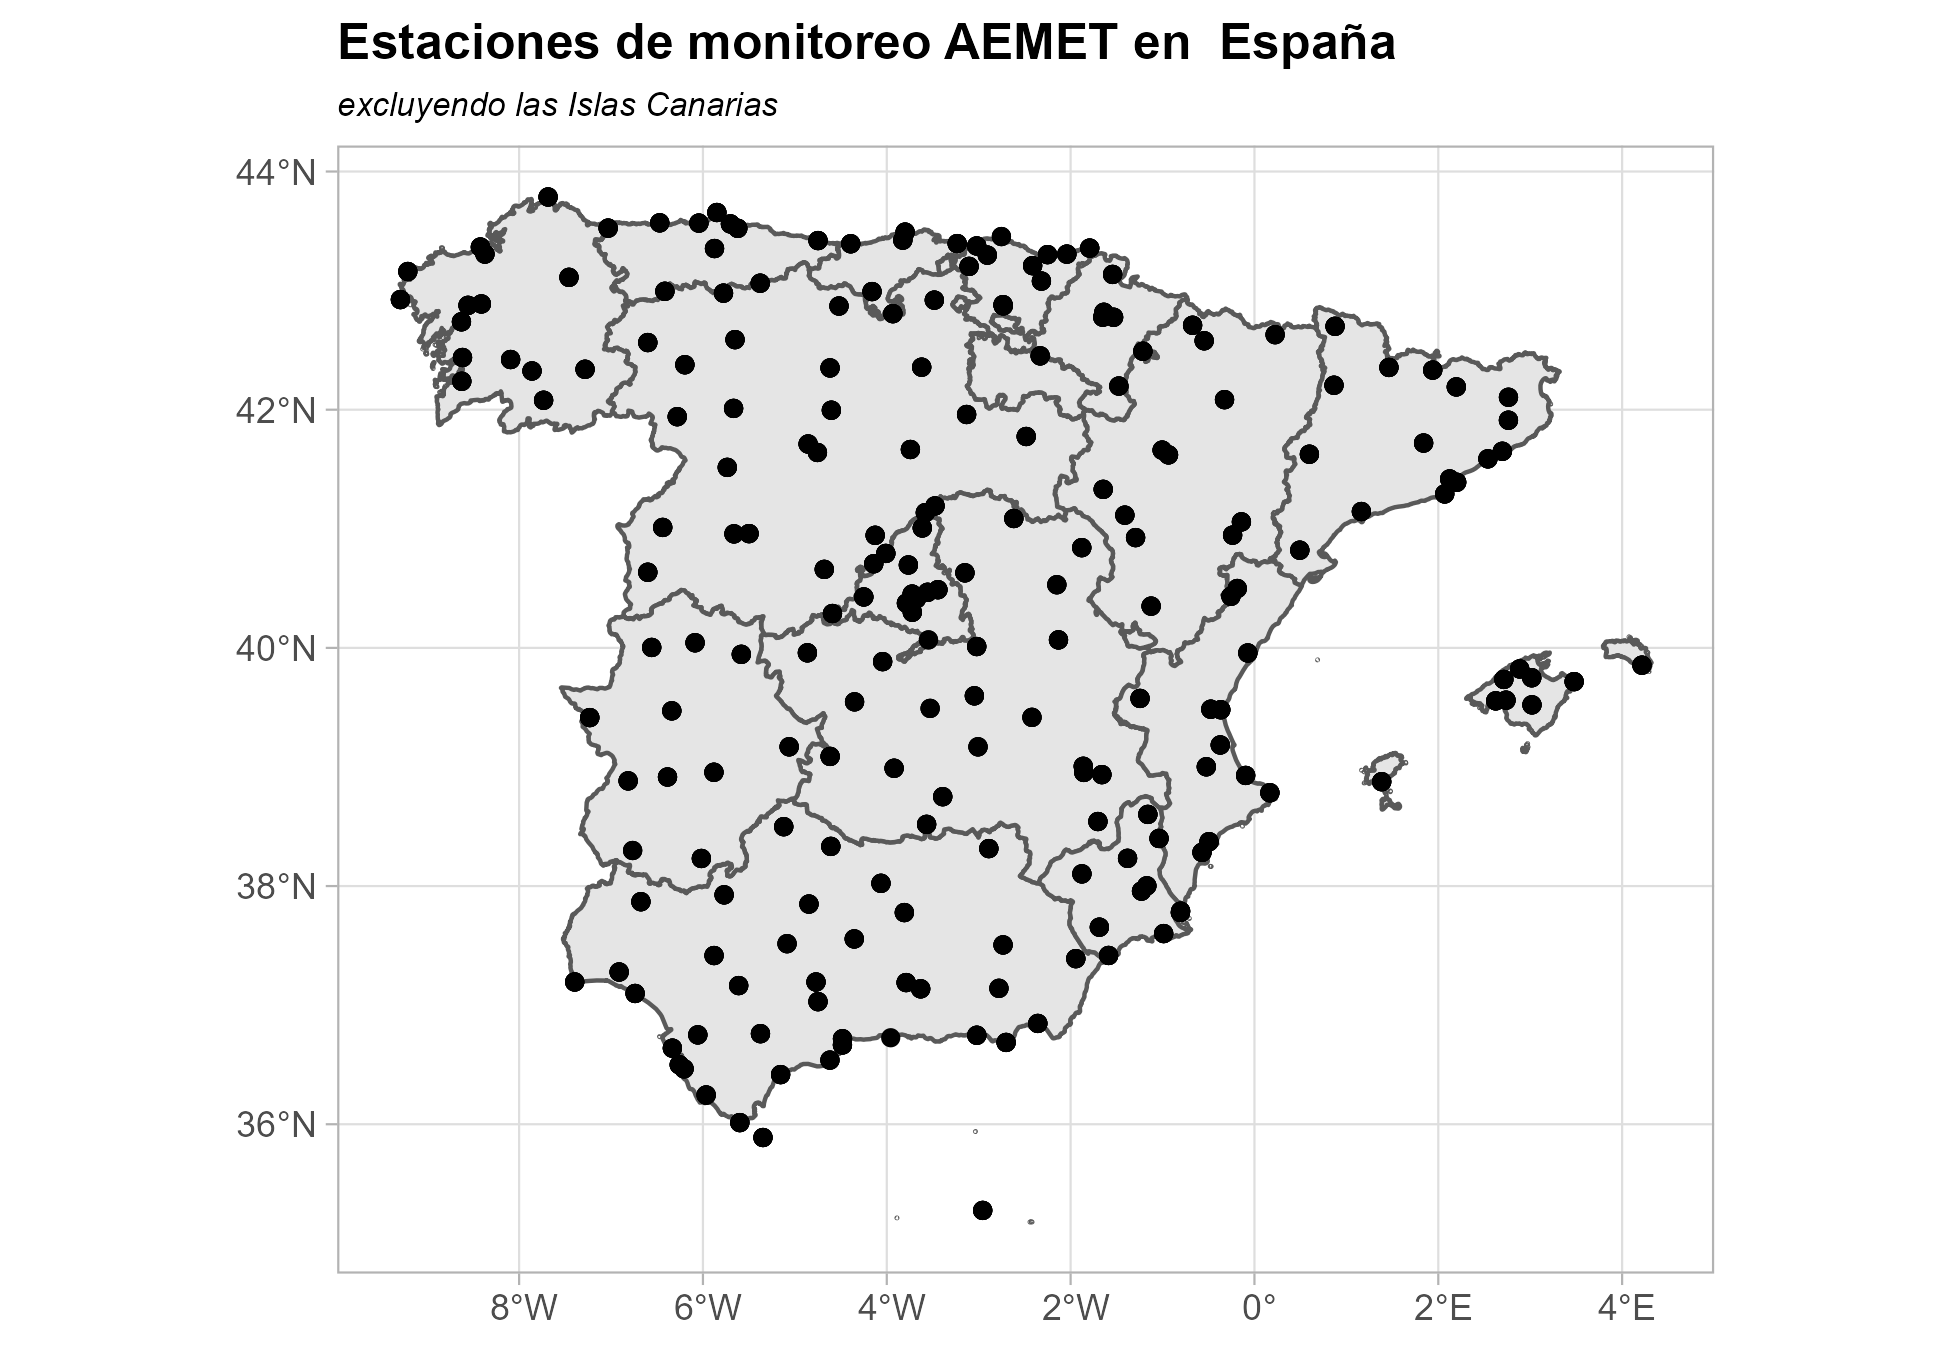
\includegraphics[width=0.6\linewidth]{_main_files/figure-latex/unnamed-chunk-13-1} 

}

\caption{Mapa con ggplot2 y lineas de nivel}\label{fig:unnamed-chunk-13}
\end{figure}

\hypertarget{renta-media-por-municipios}{%
\section{Renta media por municipios}\label{renta-media-por-municipios}}

Esta sección presenta un caso de uso en el que aprenderemos a realizar las
siguientes tareas básicas:

\begin{itemize}
\item
  Importar datos tabulares y datos espaciales.
\item
  Realizar un tratamiento de limpieza de datos y cruzar tablas.
\item
  Hacer mapas temáticos. Aprenderemos también algunas nociones básicas sobre
  cómo crear diferentes clases para un conjunto de datos continuo.
\end{itemize}

Para ello, partiremos de dos ficheros:

\begin{enumerate}
\def\labelenumi{\arabic{enumi}.}
\item
  Fichero \texttt{renta\_municipio.csv}: Este fichero contiene información de la Renta
  Neta per cápita por municipios (en euros), distritos y secciones censales.
  Esta información se ha extraído del \href{https://www.ine.es/experimental/atlas/experimental_atlas.htm}{Atlas de distribución de renta de los
  hogares}
  proporcionado por el INE, y ha sido tratado previamente para adaptar la
  información al presente ejercicio.
\item
  Fichero \texttt{municipios.gpkg}: Es un fichero que contiene datos espaciales
  (polígonos) de los municipios en España en el año 2019. Se ha extraído del
  Instituto Geográfico Nacional (IGN) usando el paquete \texttt{mapSpain}.
\end{enumerate}

\emph{Tarea 1. Importar los datos a R}

El primer paso en cualquier tipo de análisis de datos es importar los datos al
software de tratamiento (en nuestro caso, R) y analizarlos para conocer el tipo
de información que contiene:

\begin{Shaded}
\begin{Highlighting}[]
\CommentTok{\# Usaremos paquetes del tidyverse}
\FunctionTok{library}\NormalTok{(dplyr)}
\FunctionTok{library}\NormalTok{(readr)}

\NormalTok{renta }\OtherTok{\textless{}{-}} \FunctionTok{read\_csv}\NormalTok{(}\StringTok{"data/renta\_municipio.csv"}\NormalTok{, }\AttributeTok{na =} \StringTok{"."}\NormalTok{)}
\end{Highlighting}
\end{Shaded}

\begin{Shaded}
\begin{Highlighting}[]
\FunctionTok{library}\NormalTok{(sf)}
\NormalTok{munis }\OtherTok{\textless{}{-}} \FunctionTok{st\_read}\NormalTok{(}\StringTok{"data/municipios.gpkg"}\NormalTok{, }\AttributeTok{quiet =} \ConstantTok{TRUE}\NormalTok{)}
\end{Highlighting}
\end{Shaded}

\textbf{Q1: ¿Qué información tenemos sobre la variable?}

\begin{Shaded}
\begin{Highlighting}[]
\FunctionTok{head}\NormalTok{(renta)}
\CommentTok{\#\textgreater{} \# A tibble: 6 x 6}
\CommentTok{\#\textgreater{}   Unidad                          \textasciigrave{}2019\textasciigrave{} \textasciigrave{}2018\textasciigrave{} \textasciigrave{}2017\textasciigrave{} \textasciigrave{}2016\textasciigrave{} \textasciigrave{}2015\textasciigrave{}}
\CommentTok{\#\textgreater{}   \textless{}chr\textgreater{}                            \textless{}dbl\textgreater{}  \textless{}dbl\textgreater{}  \textless{}dbl\textgreater{}  \textless{}dbl\textgreater{}  \textless{}dbl\textgreater{}}
\CommentTok{\#\textgreater{} 1 44001 Ababuj                        NA     NA     NA     NA     NA}
\CommentTok{\#\textgreater{} 2 4400101 Ababuj distrito 01          NA     NA     NA     NA     NA}
\CommentTok{\#\textgreater{} 3 4400101001 Ababuj sección 01001     NA     NA     NA     NA     NA}
\CommentTok{\#\textgreater{} 4 40001 Abades                     11429  10731  10314   9816   9904}
\CommentTok{\#\textgreater{} 5 4000101 Abades distrito 01       11429  10731  10314   9816   9904}
\CommentTok{\#\textgreater{} 6 4000101001 Abades sección 01001  11429  10731  10314   9816   9904}
\end{Highlighting}
\end{Shaded}

Podemos comprobar que tenemos información para los años 2015 a 2019. Además, la
columna \texttt{Unidad} contiene un literal con el municipio o sección correspondiente.

\textbf{Q2: ¿Qué información tenemos sobre el objeto espacial?}

\begin{Shaded}
\begin{Highlighting}[]
\FunctionTok{head}\NormalTok{(munis)}
\CommentTok{\#\textgreater{} Simple feature collection with 6 features and 7 fields}
\CommentTok{\#\textgreater{} Geometry type: MULTIPOLYGON}
\CommentTok{\#\textgreater{} Dimension:     XY}
\CommentTok{\#\textgreater{} Bounding box:  xmin: {-}3.140179 ymin: 36.73817 xmax: {-}2.057058 ymax: 37.54579}
\CommentTok{\#\textgreater{} Geodetic CRS:  ETRS89}
\CommentTok{\#\textgreater{}   codauto ine.ccaa.name cpro ine.prov.name cmun      name LAU\_CODE}
\CommentTok{\#\textgreater{} 1      01     Andalucía   04       Almería  001      Abla    04001}
\CommentTok{\#\textgreater{} 2      01     Andalucía   04       Almería  002  Abrucena    04002}
\CommentTok{\#\textgreater{} 3      01     Andalucía   04       Almería  003      Adra    04003}
\CommentTok{\#\textgreater{} 4      01     Andalucía   04       Almería  004 Albanchez    04004}
\CommentTok{\#\textgreater{} 5      01     Andalucía   04       Almería  005 Alboloduy    04005}
\CommentTok{\#\textgreater{} 6      01     Andalucía   04       Almería  006     Albox    04006}
\CommentTok{\#\textgreater{}                             geom}
\CommentTok{\#\textgreater{} 1 MULTIPOLYGON ((({-}2.775594 3...}
\CommentTok{\#\textgreater{} 2 MULTIPOLYGON ((({-}2.787566 3...}
\CommentTok{\#\textgreater{} 3 MULTIPOLYGON ((({-}3.051988 3...}
\CommentTok{\#\textgreater{} 4 MULTIPOLYGON ((({-}2.181086 3...}
\CommentTok{\#\textgreater{} 5 MULTIPOLYGON ((({-}2.572442 3...}
\CommentTok{\#\textgreater{} 6 MULTIPOLYGON ((({-}2.128106 3...}
\end{Highlighting}
\end{Shaded}

Podemos comprobar que \texttt{munis} es un objeto que contiene Polígonos y varias
columnas, entre ellas dos especialmente relevantes: \texttt{cpro} y \texttt{cmun}, que
corresponden a los códigos de provincia y de municipio respectivamente. Podemos
comprobar que este código también se encuentra en nuestro dataset \texttt{renta}.

\emph{Tarea 2. Comprobamos campos en común para un municipio: Noblejas}

\begin{Shaded}
\begin{Highlighting}[]
\CommentTok{\# Miro un municipio: Noblejas}

\NormalTok{renta[}\FunctionTok{grep}\NormalTok{(}\StringTok{"Noblejas"}\NormalTok{, renta}\SpecialCharTok{$}\NormalTok{Unidad), ]}
\CommentTok{\#\textgreater{} \# A tibble: 5 x 6}
\CommentTok{\#\textgreater{}   Unidad                            \textasciigrave{}2019\textasciigrave{} \textasciigrave{}2018\textasciigrave{} \textasciigrave{}2017\textasciigrave{} \textasciigrave{}2016\textasciigrave{} \textasciigrave{}2015\textasciigrave{}}
\CommentTok{\#\textgreater{}   \textless{}chr\textgreater{}                              \textless{}dbl\textgreater{}  \textless{}dbl\textgreater{}  \textless{}dbl\textgreater{}  \textless{}dbl\textgreater{}  \textless{}dbl\textgreater{}}
\CommentTok{\#\textgreater{} 1 45115 Noblejas                     10591  10314   9751   9484   9124}
\CommentTok{\#\textgreater{} 2 4511501 Noblejas distrito 01       11039  10717  10135   9711   9386}
\CommentTok{\#\textgreater{} 3 4511501001 Noblejas sección 01001  11039  10717  10135   9711   9386}
\CommentTok{\#\textgreater{} 4 4511502 Noblejas distrito 02       10276  10029   9475   9319   8938}
\CommentTok{\#\textgreater{} 5 4511502001 Noblejas sección 02001  10276  10029   9475   9319   8938}

\NormalTok{munis[}\FunctionTok{grep}\NormalTok{(}\StringTok{"Noblejas"}\NormalTok{, munis}\SpecialCharTok{$}\NormalTok{name), }\FunctionTok{c}\NormalTok{(}\StringTok{"name"}\NormalTok{, }\StringTok{"cpro"}\NormalTok{, }\StringTok{"cmun"}\NormalTok{)]}
\CommentTok{\#\textgreater{} Simple feature collection with 1 feature and 3 fields}
\CommentTok{\#\textgreater{} Geometry type: MULTIPOLYGON}
\CommentTok{\#\textgreater{} Dimension:     XY}
\CommentTok{\#\textgreater{} Bounding box:  xmin: {-}3.489824 ymin: 39.93003 xmax: {-}3.372611 ymax: 40.05017}
\CommentTok{\#\textgreater{} Geodetic CRS:  ETRS89}
\CommentTok{\#\textgreater{}          name cpro cmun                           geom}
\CommentTok{\#\textgreater{} 4985 Noblejas   45  115 MULTIPOLYGON ((({-}3.44681 40...}
\end{Highlighting}
\end{Shaded}

En el caso de Noblejas, el código completo es 45115. Sin embargo, en el caso de
la tabla \texttt{renta}, debemos extraer ese valor del literal. Para ello debemos
manipular la columna y extraer la primera palabra de la columna \texttt{Unidad}:

\begin{Shaded}
\begin{Highlighting}[]

\CommentTok{\# Creo una función y la aplico a toda la columna}
\NormalTok{extrae\_codigo }\OtherTok{\textless{}{-}} \ControlFlowTok{function}\NormalTok{(x) \{}
  \FunctionTok{unlist}\NormalTok{(}\FunctionTok{strsplit}\NormalTok{(x, }\StringTok{" "}\NormalTok{))[}\DecValTok{1}\NormalTok{]}
\NormalTok{\}}

\NormalTok{renta}\SpecialCharTok{$}\NormalTok{codigo\_ine }\OtherTok{\textless{}{-}} \FunctionTok{sapply}\NormalTok{(}\FunctionTok{as.character}\NormalTok{(renta}\SpecialCharTok{$}\NormalTok{Unidad), extrae\_codigo)}

\FunctionTok{head}\NormalTok{(renta[}\FunctionTok{c}\NormalTok{(}\StringTok{"Unidad"}\NormalTok{, }\StringTok{"codigo\_ine"}\NormalTok{)])}
\CommentTok{\#\textgreater{} \# A tibble: 6 x 2}
\CommentTok{\#\textgreater{}   Unidad                          codigo\_ine}
\CommentTok{\#\textgreater{}   \textless{}chr\textgreater{}                           \textless{}chr\textgreater{}     }
\CommentTok{\#\textgreater{} 1 44001 Ababuj                    44001     }
\CommentTok{\#\textgreater{} 2 4400101 Ababuj distrito 01      4400101   }
\CommentTok{\#\textgreater{} 3 4400101001 Ababuj sección 01001 4400101001}
\CommentTok{\#\textgreater{} 4 40001 Abades                    40001     }
\CommentTok{\#\textgreater{} 5 4000101 Abades distrito 01      4000101   }
\CommentTok{\#\textgreater{} 6 4000101001 Abades sección 01001 4000101001}
\end{Highlighting}
\end{Shaded}

Ahora, es necesario crear la misma variable en \texttt{munis} para poder realizar el
cruce:

\begin{Shaded}
\begin{Highlighting}[]

\NormalTok{munis}\SpecialCharTok{$}\NormalTok{codigo\_ine }\OtherTok{\textless{}{-}} \FunctionTok{paste0}\NormalTok{(munis}\SpecialCharTok{$}\NormalTok{cpro, munis}\SpecialCharTok{$}\NormalTok{cmun)}

\FunctionTok{head}\NormalTok{(munis[, }\FunctionTok{c}\NormalTok{(}\StringTok{"name"}\NormalTok{, }\StringTok{"codigo\_ine"}\NormalTok{)])}
\CommentTok{\#\textgreater{} Simple feature collection with 6 features and 2 fields}
\CommentTok{\#\textgreater{} Geometry type: MULTIPOLYGON}
\CommentTok{\#\textgreater{} Dimension:     XY}
\CommentTok{\#\textgreater{} Bounding box:  xmin: {-}3.140179 ymin: 36.73817 xmax: {-}2.057058 ymax: 37.54579}
\CommentTok{\#\textgreater{} Geodetic CRS:  ETRS89}
\CommentTok{\#\textgreater{}        name codigo\_ine                           geom}
\CommentTok{\#\textgreater{} 1      Abla      04001 MULTIPOLYGON ((({-}2.775594 3...}
\CommentTok{\#\textgreater{} 2  Abrucena      04002 MULTIPOLYGON ((({-}2.787566 3...}
\CommentTok{\#\textgreater{} 3      Adra      04003 MULTIPOLYGON ((({-}3.051988 3...}
\CommentTok{\#\textgreater{} 4 Albanchez      04004 MULTIPOLYGON ((({-}2.181086 3...}
\CommentTok{\#\textgreater{} 5 Alboloduy      04005 MULTIPOLYGON ((({-}2.572442 3...}
\CommentTok{\#\textgreater{} 6     Albox      04006 MULTIPOLYGON ((({-}2.128106 3...}
\end{Highlighting}
\end{Shaded}

\emph{Tarea 3: Unimos los objetos renta y mapas con la función \texttt{left\_join}}

Ya estamos listos para realizar el cruce. Además, seleccionaremos sólo las
columnas que vamos a usar, en este caso la del año 2019:

\begin{Shaded}
\begin{Highlighting}[]

\NormalTok{munis\_renta }\OtherTok{\textless{}{-}}\NormalTok{ munis }\SpecialCharTok{\%\textgreater{}\%}
  \FunctionTok{left\_join}\NormalTok{(renta) }\SpecialCharTok{\%\textgreater{}\%}
\NormalTok{  dplyr}\SpecialCharTok{::}\FunctionTok{select}\NormalTok{(name, cpro, cmun, }\StringTok{\textasciigrave{}}\AttributeTok{2019}\StringTok{\textasciigrave{}}\NormalTok{)}
\end{Highlighting}
\end{Shaded}

\textbf{Cuando crucemos datos espaciales con datos no espaciales en R, es importante
que el primer dataset sea el que contiene los datos espaciales}. Esto es así
porque el objeto resultante ``hereda'' la clase del primer objeto.

\textbf{Q3: ¿Qué ocurre si realizáramos el proceso poniendo los datos espaciales en el
lado derecho del join?}

A modo de ejemplo, si realizáramos el proceso poniendo los datos espaciales en
el lado derecho del join, los datos finales no serán espaciales:

\begin{Shaded}
\begin{Highlighting}[]

\CommentTok{\# Miramos la clase de munis\_renta}

\FunctionTok{class}\NormalTok{(munis\_renta)}
\CommentTok{\#\textgreater{} [1] "sf"         "data.frame"}

\CommentTok{\# Es un sf, por tanto espacial}

\CommentTok{\# ¿Que pasa si realizamos el cruce de la otra manera?}
\NormalTok{renta }\SpecialCharTok{\%\textgreater{}\%}
  \FunctionTok{left\_join}\NormalTok{(munis) }\SpecialCharTok{\%\textgreater{}\%}
\NormalTok{  dplyr}\SpecialCharTok{::}\FunctionTok{select}\NormalTok{(name, cpro, cmun, }\StringTok{\textasciigrave{}}\AttributeTok{2019}\StringTok{\textasciigrave{}}\NormalTok{) }\SpecialCharTok{\%\textgreater{}\%}
  \FunctionTok{class}\NormalTok{()}
\CommentTok{\#\textgreater{} [1] "tbl\_df"     "tbl"        "data.frame"}
\end{Highlighting}
\end{Shaded}

El resultado es un tibble o data.frame, \textbf{¡pero no es espacial!}

\emph{Tarea 4. Histograma de la distribución de la renta}

Una vez que tenemos los datos unidos podemos realizar algunos análisis básicos,
como la realización de un histograma

\begin{Shaded}
\begin{Highlighting}[]

\FunctionTok{library}\NormalTok{(ggplot2)}

\NormalTok{munis\_renta }\SpecialCharTok{\%\textgreater{}\%}
  \FunctionTok{ggplot}\NormalTok{(}\FunctionTok{aes}\NormalTok{(}\AttributeTok{x =} \StringTok{\textasciigrave{}}\AttributeTok{2019}\StringTok{\textasciigrave{}}\NormalTok{)) }\SpecialCharTok{+}
  \FunctionTok{geom\_histogram}\NormalTok{(}\AttributeTok{color =} \StringTok{"darkblue"}\NormalTok{, }\AttributeTok{fill =} \StringTok{"lightblue"}\NormalTok{) }\SpecialCharTok{+}
  \FunctionTok{scale\_x\_continuous}\NormalTok{(}\AttributeTok{labels =}\NormalTok{ scales}\SpecialCharTok{::}\FunctionTok{label\_number\_auto}\NormalTok{()) }\SpecialCharTok{+}
  \FunctionTok{scale\_y\_continuous}\NormalTok{(}\AttributeTok{labels =}\NormalTok{ scales}\SpecialCharTok{::}\FunctionTok{label\_percent}\NormalTok{()) }\SpecialCharTok{+}
  \FunctionTok{labs}\NormalTok{(}
    \AttributeTok{y =} \StringTok{""}\NormalTok{,}
    \AttributeTok{x =} \StringTok{"Renta neta media por persona (€)"}
\NormalTok{  )}
\end{Highlighting}
\end{Shaded}

\begin{center}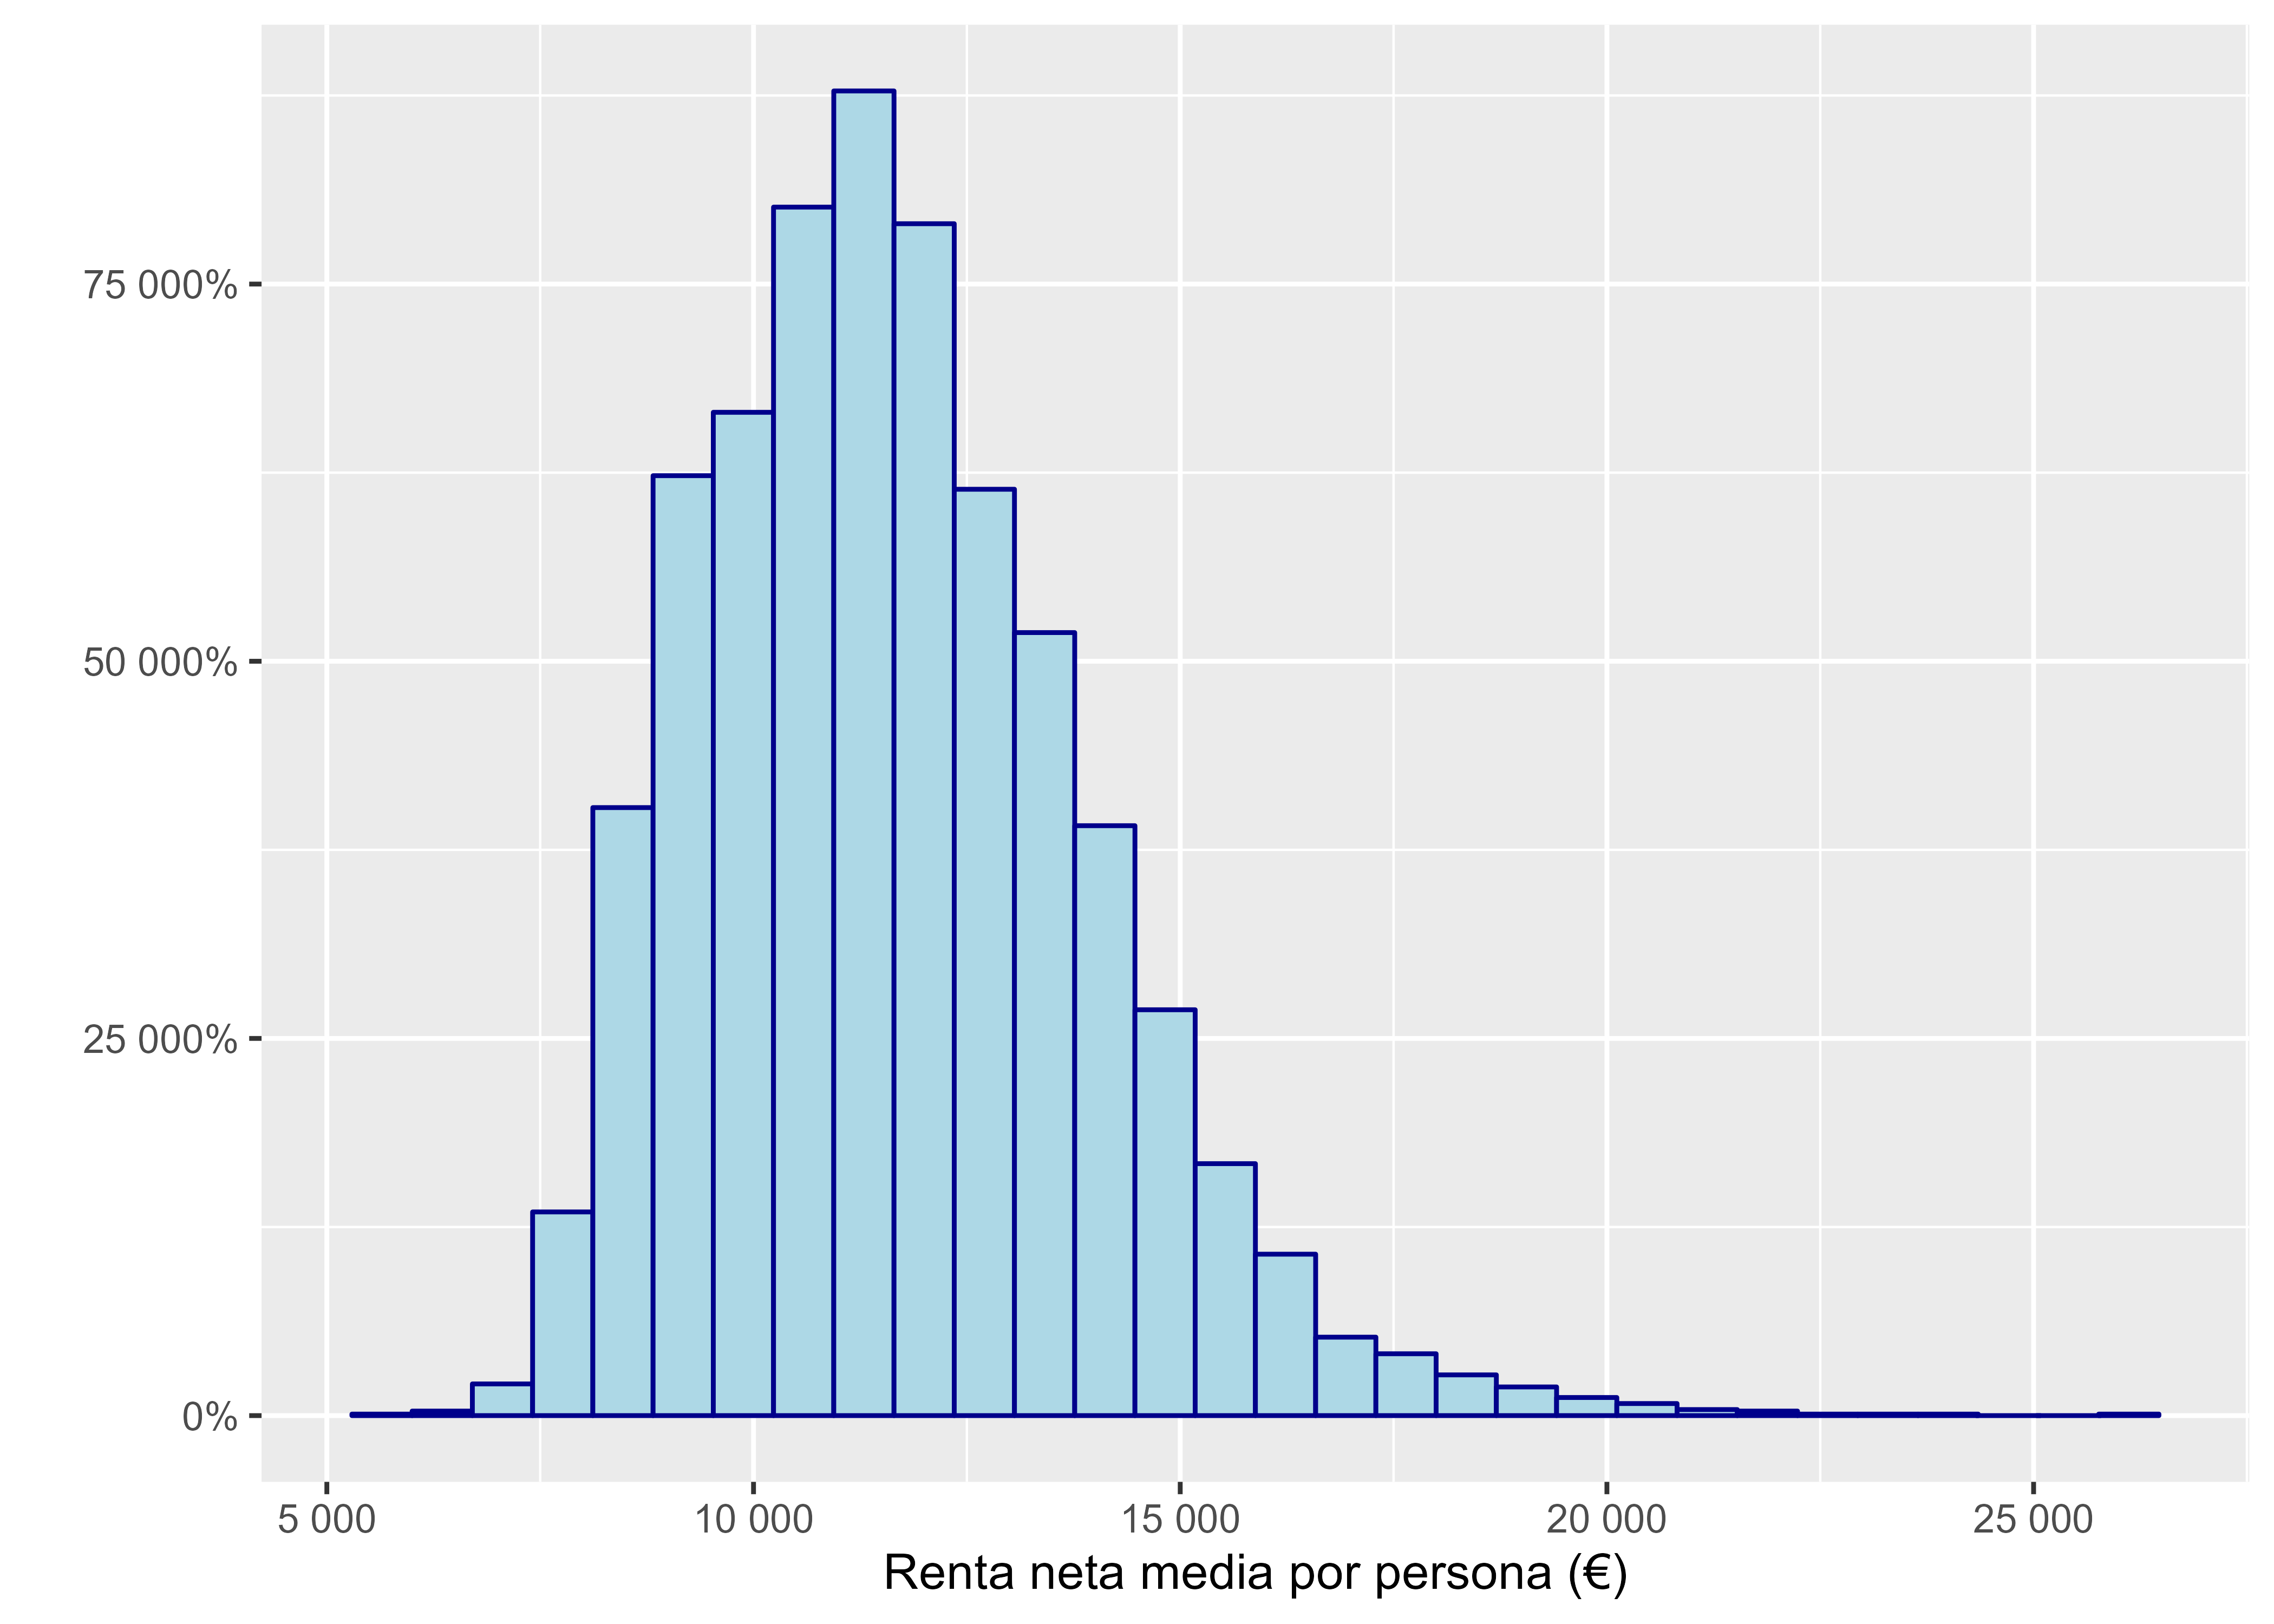
\includegraphics[width=0.6\linewidth]{_main_files/figure-latex/basic-1} \end{center}

Podemos observar que la renta presenta una distribución Gamma con un gran de
municipios concentrados en zonas medias de renta y pocos municipios en tramos de
rentas altas. Como veremos más adelante, esta distribución va a afectar a la
información que transmite el mapa.

\emph{Tarea 5. Mapa de coropletas de la distribución de la renta}

Vamos a realizar ahora un mapa de coropletas mostrando la distribución de la
renta usando los valores brutos de renta sin modificar:

\begin{Shaded}
\begin{Highlighting}[]

\FunctionTok{ggplot}\NormalTok{(munis\_renta) }\SpecialCharTok{+}
  \CommentTok{\# Usamos geom\_sf, y como aes() lo que queremos mostrar, en este caso, el}
  \CommentTok{\# color del polígono representa la renta. Vamos a retirar los bordes con}
  \CommentTok{\# color = NA}
  \FunctionTok{geom\_sf}\NormalTok{(}\FunctionTok{aes}\NormalTok{(}\AttributeTok{fill =} \StringTok{\textasciigrave{}}\AttributeTok{2019}\StringTok{\textasciigrave{}}\NormalTok{), }\AttributeTok{color =} \ConstantTok{NA}\NormalTok{) }\SpecialCharTok{+}
  \FunctionTok{theme\_minimal}\NormalTok{() }\SpecialCharTok{+}
  \FunctionTok{scale\_fill\_continuous}\NormalTok{(}\AttributeTok{labels =}\NormalTok{ scales}\SpecialCharTok{::}\FunctionTok{label\_number}\NormalTok{(}
    \AttributeTok{big.mark =} \StringTok{"."}\NormalTok{,}
    \AttributeTok{decimal.mark =} \StringTok{","}\NormalTok{,}
    \AttributeTok{suffix =} \StringTok{" €"}
\NormalTok{  )) }\SpecialCharTok{+}
  \FunctionTok{labs}\NormalTok{(}
    \AttributeTok{title =} \StringTok{"Renta neta media por persona"}\NormalTok{,}
    \AttributeTok{caption =} \StringTok{"Datos: INE"}
\NormalTok{  )}
\end{Highlighting}
\end{Shaded}

\begin{center}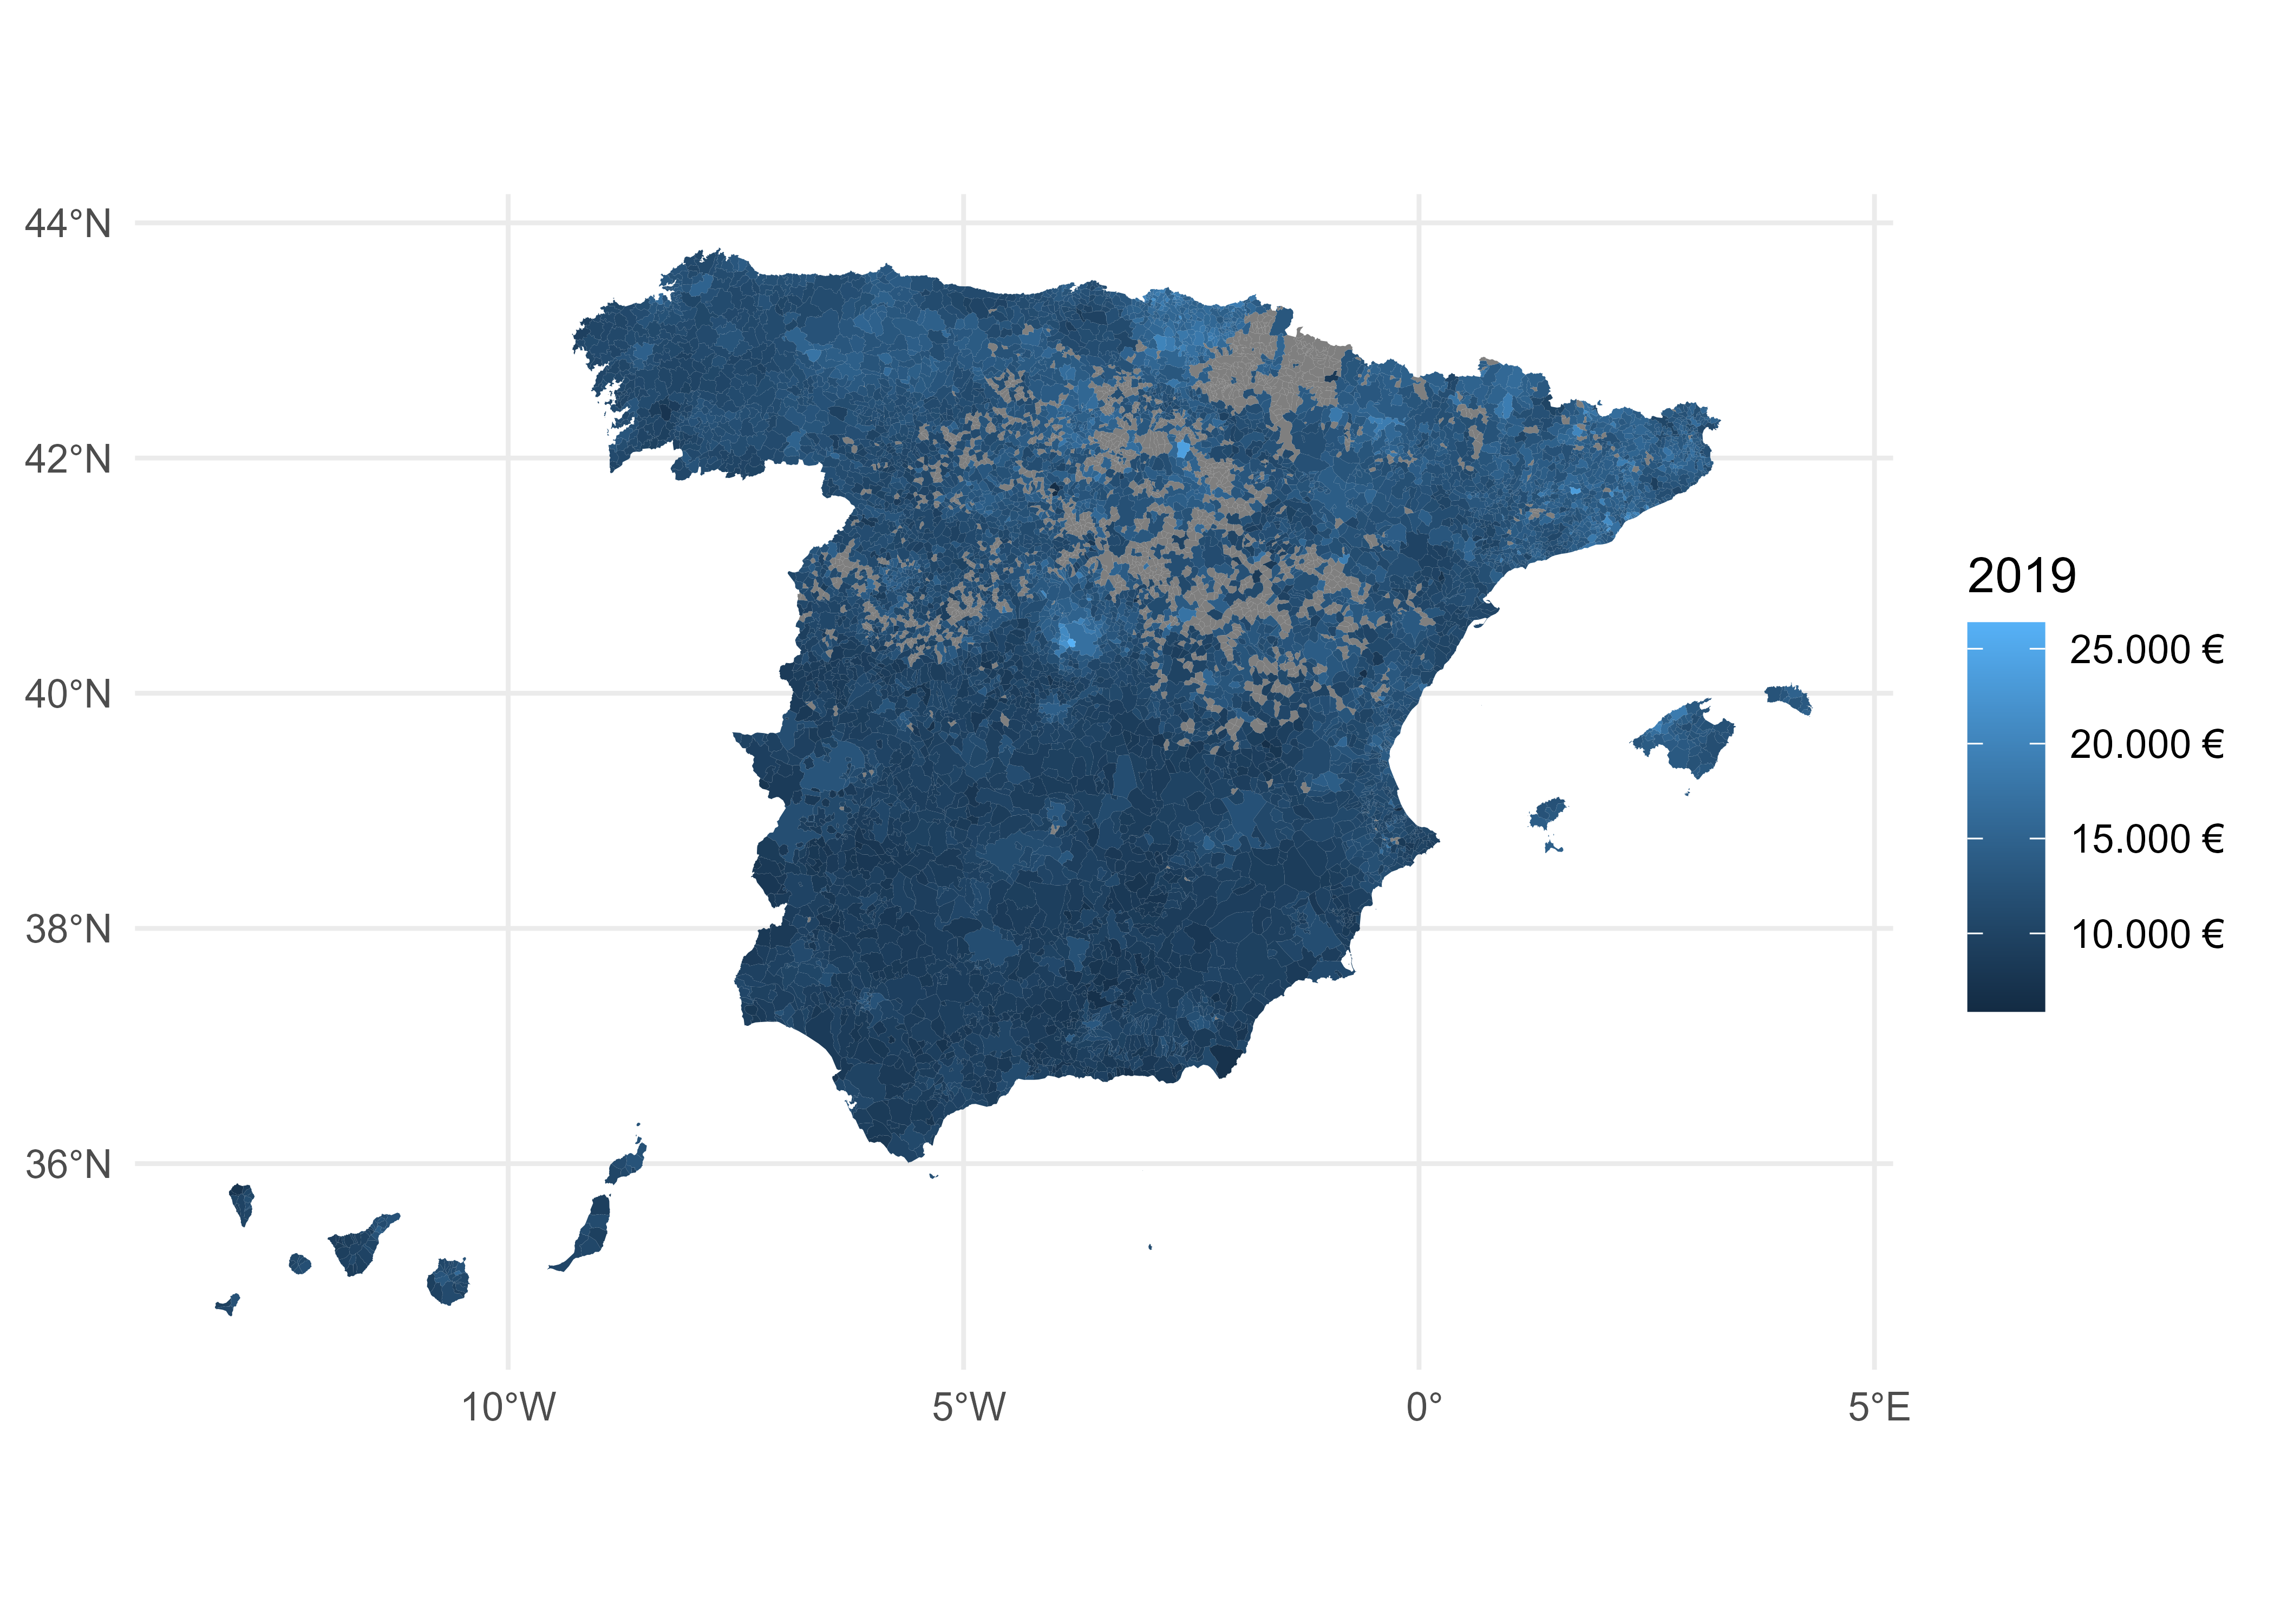
\includegraphics[width=0.6\linewidth]{_main_files/figure-latex/maparenta1-1} \end{center}

Este primer mapa no es demasiado informativo, por los siguientes motivos:

\begin{itemize}
\item
  Existe una serie de municipios para los que no tenemos datos.
\item
  La escala de color no es la más adecuada.
\item
  Dada la distribución de los datos, puede ser adecuado crear grupos de renta
  para que el mapa sea más interpretable.
\end{itemize}

\emph{Tarea 6. Eliminamos los municipios sin datos y cambiamos la escala de color}

Vamos a probar a eliminar los municipios sin datos y a cambiar la escala de
color para ver si mejora la visualización.

\begin{Shaded}
\begin{Highlighting}[]

\NormalTok{munis\_renta\_clean }\OtherTok{\textless{}{-}}\NormalTok{ munis\_renta }\SpecialCharTok{\%\textgreater{}\%} \FunctionTok{filter}\NormalTok{(}\SpecialCharTok{!}\FunctionTok{is.na}\NormalTok{(}\StringTok{\textasciigrave{}}\AttributeTok{2019}\StringTok{\textasciigrave{}}\NormalTok{))}

\FunctionTok{ggplot}\NormalTok{(munis\_renta\_clean) }\SpecialCharTok{+}
  \FunctionTok{geom\_sf}\NormalTok{(}\FunctionTok{aes}\NormalTok{(}\AttributeTok{fill =} \StringTok{\textasciigrave{}}\AttributeTok{2019}\StringTok{\textasciigrave{}}\NormalTok{), }\AttributeTok{color =} \ConstantTok{NA}\NormalTok{) }\SpecialCharTok{+}
  \CommentTok{\# Cambiamos la paleta de colores, vamos a usar una paleta denominada Inferno,}
  \CommentTok{\# ya incluida en base R con hcl.colors}

  \CommentTok{\# Como son datos continuos, puedo usar Inferno}
  \FunctionTok{scale\_fill\_gradientn}\NormalTok{(}
    \AttributeTok{colours =} \FunctionTok{hcl.colors}\NormalTok{(}\DecValTok{20}\NormalTok{, }\StringTok{"Inferno"}\NormalTok{, }\AttributeTok{rev =} \ConstantTok{TRUE}\NormalTok{),}
    \AttributeTok{labels =}\NormalTok{ scales}\SpecialCharTok{::}\FunctionTok{label\_number}\NormalTok{(}
      \AttributeTok{big.mark =} \StringTok{"."}\NormalTok{,}
      \AttributeTok{decimal.mark =} \StringTok{","}\NormalTok{,}
      \AttributeTok{suffix =} \StringTok{" €"}
\NormalTok{    )}
\NormalTok{  ) }\SpecialCharTok{+}
  \FunctionTok{theme\_minimal}\NormalTok{() }\SpecialCharTok{+}
  \FunctionTok{labs}\NormalTok{(}
    \AttributeTok{title =} \StringTok{"Renta neta media por persona"}\NormalTok{,}
    \AttributeTok{caption =} \StringTok{"Datos: INE"}
\NormalTok{  )}
\end{Highlighting}
\end{Shaded}

\begin{center}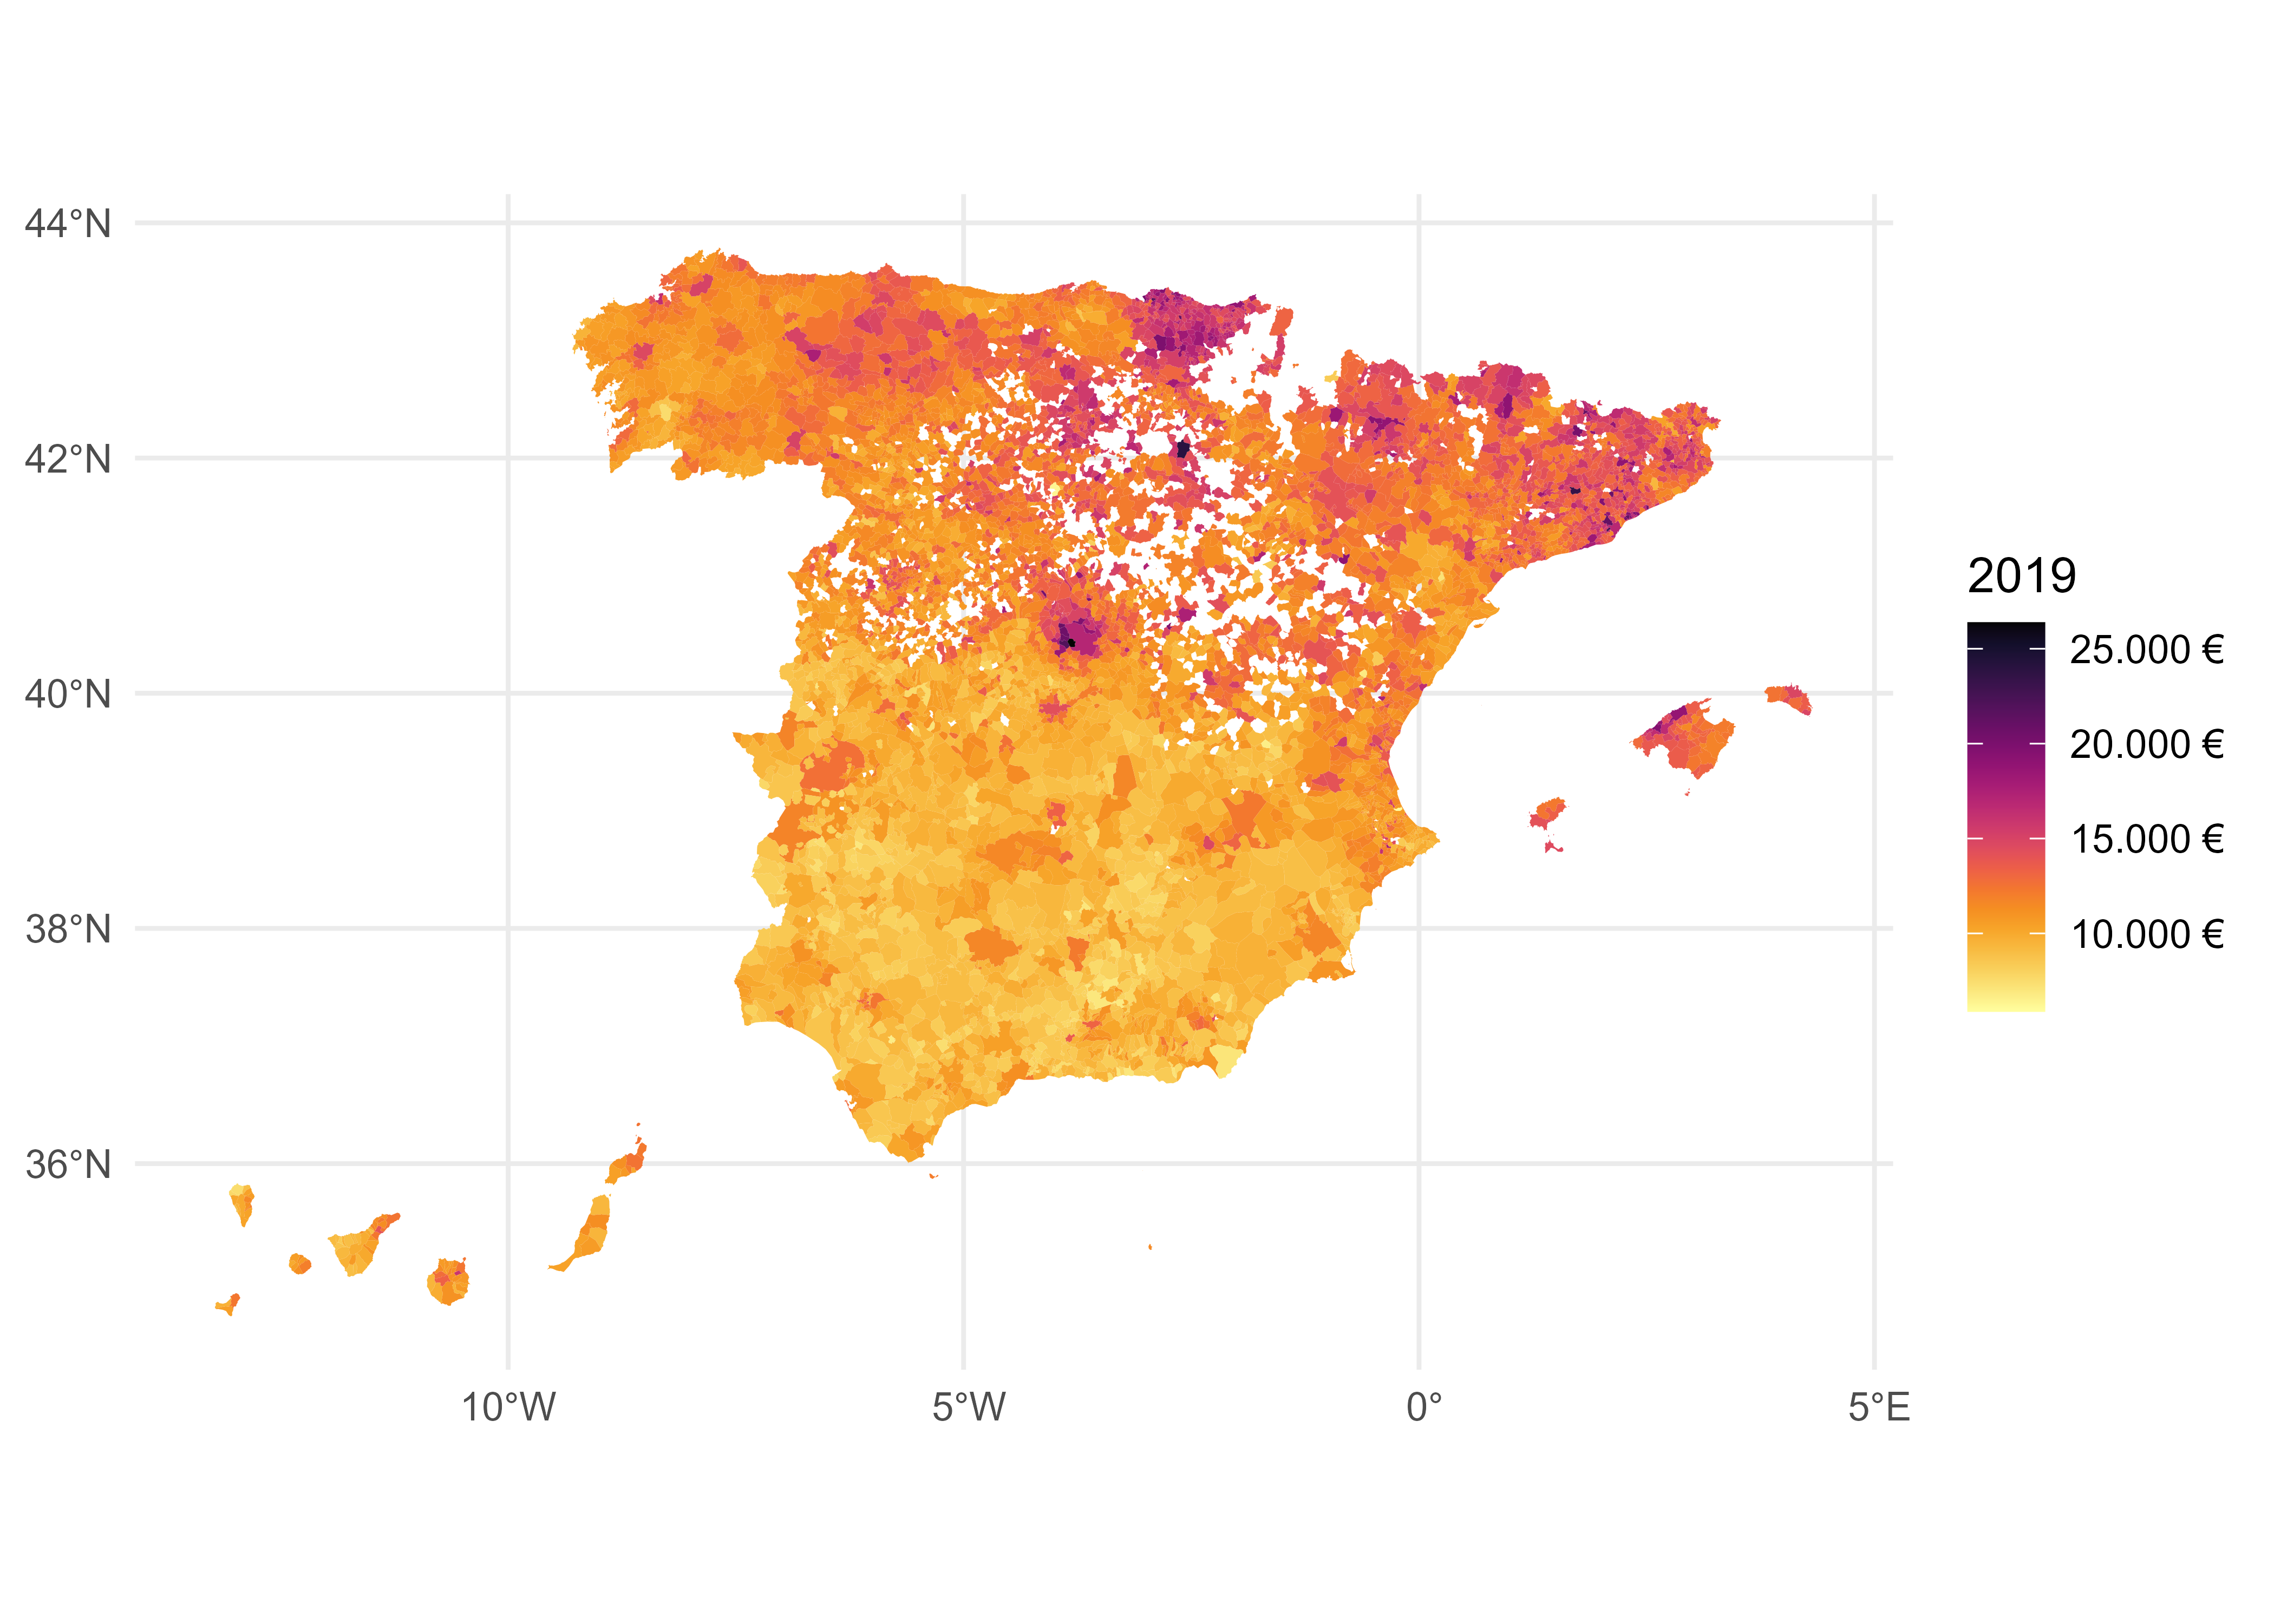
\includegraphics[width=0.6\linewidth]{_main_files/figure-latex/maparenta2-1} \end{center}

Este mapa nos da algo más de información, y parece intuirse que las rentas más
altas se encuentran en zonas de País Vasco, Madrid y Cataluña. Sin embargo, el
hecho de que la distribución de los datos no sea normal está afectando a la
visualización.

\emph{Tarea 7. Agrupar los datos en clases para mejorar la visualización}

Para intentar atajar este problema, podemos dividir nuestros datos en clases,
por ejemplo cuartiles o deciles. Existen varios métodos de clasificación de
datos, que en R se encuentran implementados en el paquete \texttt{classInt}. A
continuación vamos a plantear diversos métodos de clasificación y observar cómo
la ``historia'' que cuenta el mapa varía en función de dichas clases. En este
ejemplo planteamos los siguientes métodos de clasificación:

\begin{itemize}
\item
  El método de deciles: consiste en crear 10 categorías incluyendo el mismo
  número de registros en cada una de ellas.
\item
  El método de intervalos equivalentes: divide el rango de valores en un
  número de grupos definido. La distancia de todos los intervalos es idéntica,
  por lo que este método no tiene en cuenta la distribución de los registros.
\item
  El método de Fisher-Jenks: desarrollado específicamente para la
  clasificación de datos espaciales y su visualización en mapas. Produce
  agrupaciones de tal manera que los datos de cada grupo son ``cercanas'' entre
  sí y sustancialmente distintas de los valores de otros grupos.
\end{itemize}

\begin{Shaded}
\begin{Highlighting}[]

\FunctionTok{library}\NormalTok{(classInt)}
\CommentTok{\# Vamos a probar 3 métodos de clasificación: Deciles, tramos de Renta}
\CommentTok{\# equidistantes y Fisher and Jenks}

\NormalTok{deciles }\OtherTok{\textless{}{-}} \FunctionTok{classIntervals}\NormalTok{(munis\_renta\_clean}\SpecialCharTok{$}\StringTok{\textasciigrave{}}\AttributeTok{2019}\StringTok{\textasciigrave{}}\NormalTok{,}
  \AttributeTok{style =} \StringTok{"quantile"}\NormalTok{, }\AttributeTok{n =} \DecValTok{10}
\NormalTok{)}
\NormalTok{deciles}
\CommentTok{\#\textgreater{} style: quantile}
\CommentTok{\#\textgreater{}     [5898,8935.6)   [8935.6,9662.2)  [9662.2,10352.8)   [10352.8,10918) }
\CommentTok{\#\textgreater{}               656               656               655               654 }
\CommentTok{\#\textgreater{}     [10918,11462)   [11462,11998.6) [11998.6,12651.4) [12651.4,13475.8) }
\CommentTok{\#\textgreater{}               655               658               656               655 }
\CommentTok{\#\textgreater{} [13475.8,14618.4)   [14618.4,26367] }
\CommentTok{\#\textgreater{}               656               656}
\FunctionTok{plot}\NormalTok{(deciles, }\AttributeTok{pal =} \FunctionTok{hcl.colors}\NormalTok{(}\DecValTok{20}\NormalTok{, }\StringTok{"Inferno"}\NormalTok{), }\AttributeTok{main =} \StringTok{"Deciles"}\NormalTok{)}
\end{Highlighting}
\end{Shaded}

\begin{center}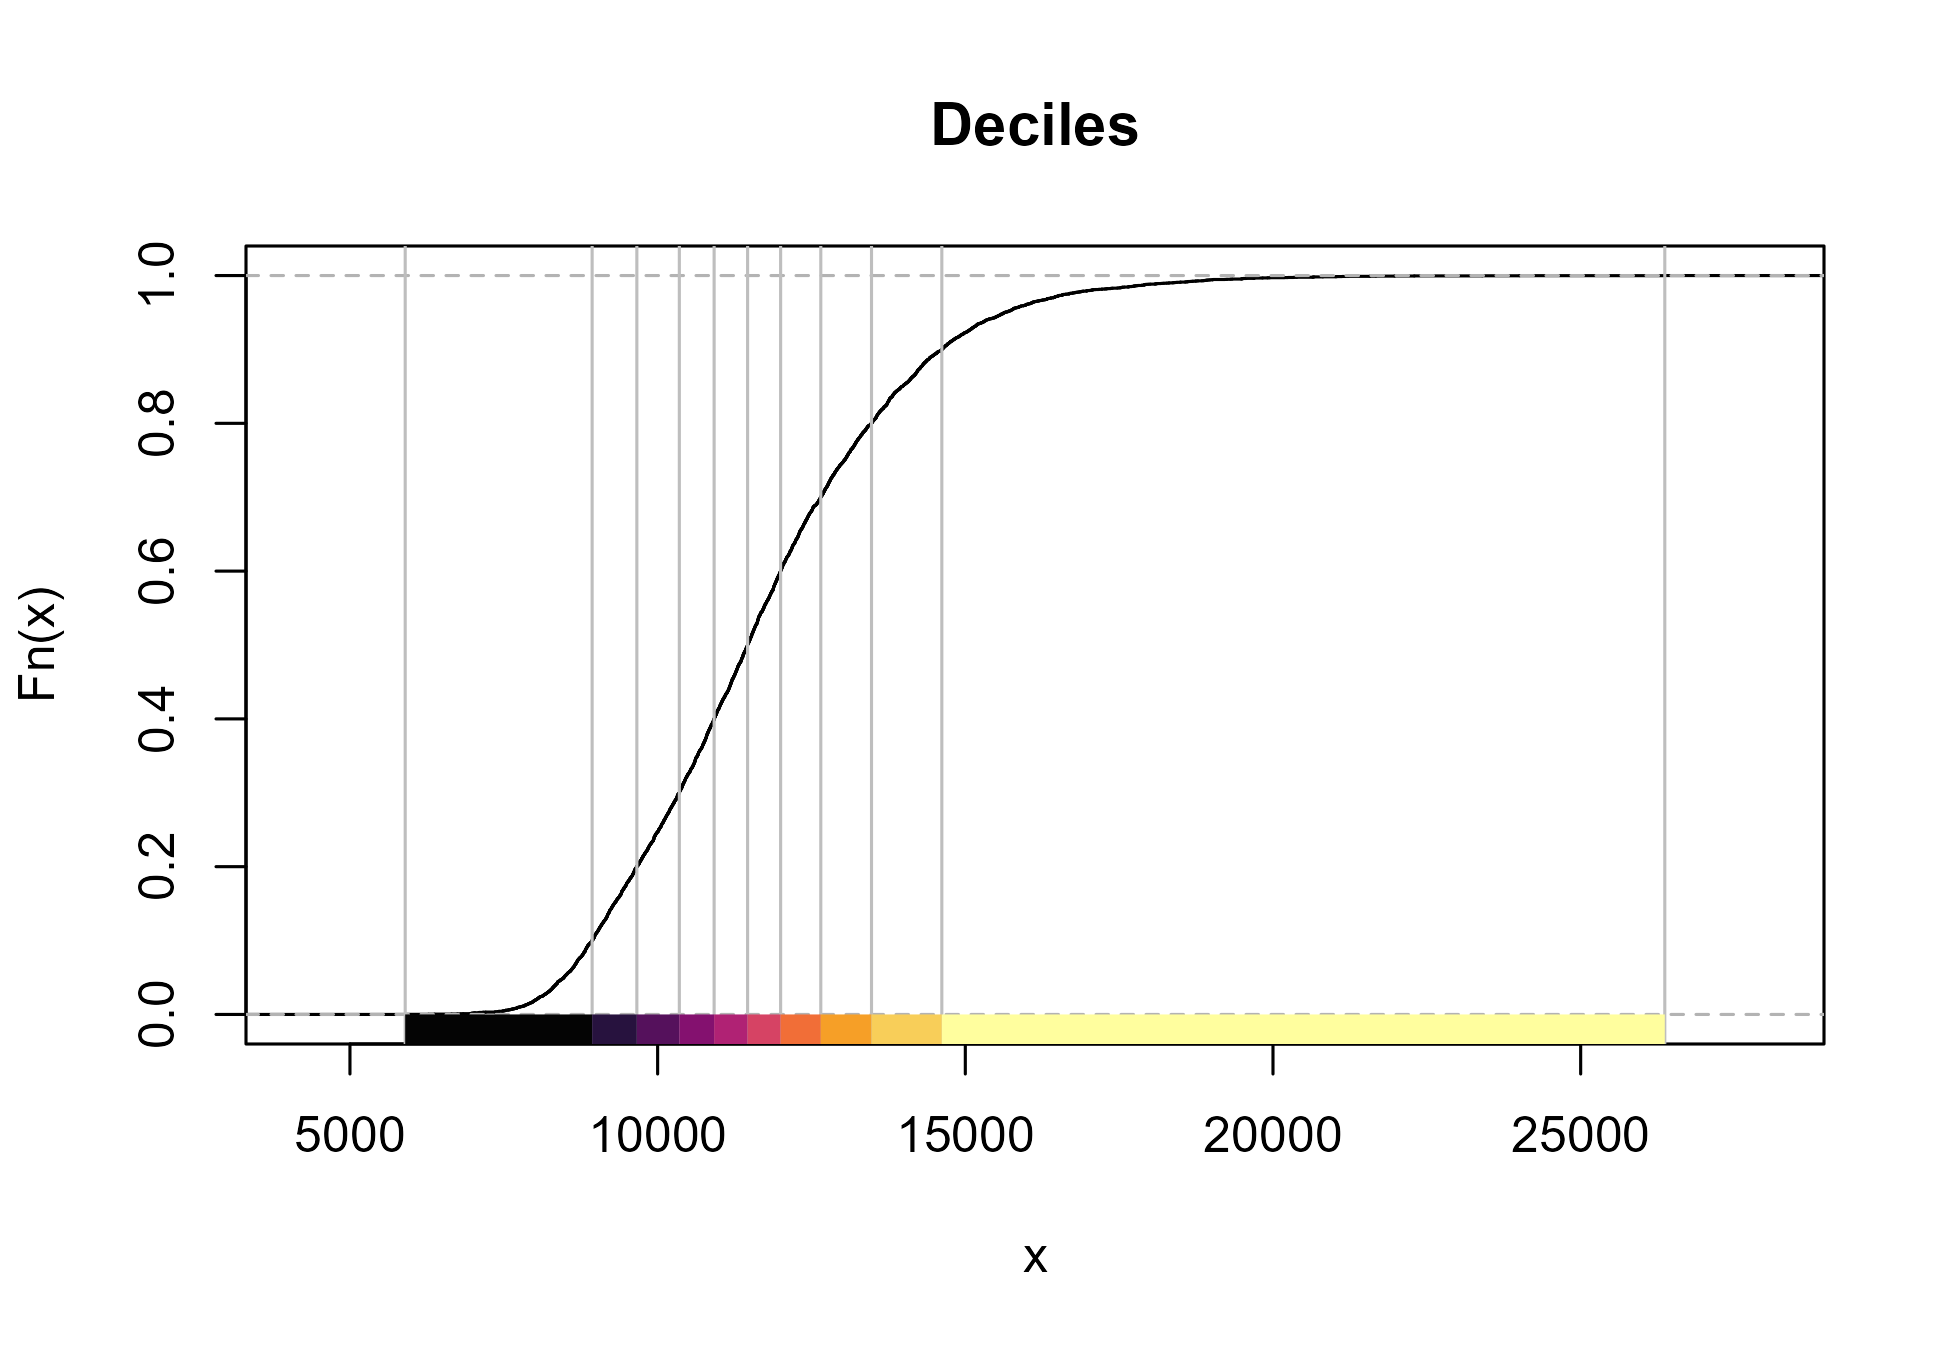
\includegraphics[width=0.6\linewidth]{_main_files/figure-latex/classint-1} \end{center}

\begin{Shaded}
\begin{Highlighting}[]


\CommentTok{\# Tramos equidistantes en términos de renta}
\NormalTok{equal }\OtherTok{\textless{}{-}} \FunctionTok{classIntervals}\NormalTok{(munis\_renta\_clean}\SpecialCharTok{$}\StringTok{\textasciigrave{}}\AttributeTok{2019}\StringTok{\textasciigrave{}}\NormalTok{,}
  \AttributeTok{style =} \StringTok{"equal"}\NormalTok{, }\AttributeTok{n =} \DecValTok{10}
\NormalTok{)}
\NormalTok{equal}
\CommentTok{\#\textgreater{} style: equal}
\CommentTok{\#\textgreater{}     [5898,7944.9)   [7944.9,9991.8)  [9991.8,12038.7) [12038.7,14085.6) }
\CommentTok{\#\textgreater{}               103              1510              2374              1637 }
\CommentTok{\#\textgreater{} [14085.6,16132.5) [16132.5,18179.4) [18179.4,20226.3) [20226.3,22273.2) }
\CommentTok{\#\textgreater{}               702               161                52                14 }
\CommentTok{\#\textgreater{} [22273.2,24320.1)   [24320.1,26367] }
\CommentTok{\#\textgreater{}                 3                 1}
\FunctionTok{plot}\NormalTok{(equal, }\AttributeTok{pal =} \FunctionTok{hcl.colors}\NormalTok{(}\DecValTok{20}\NormalTok{, }\StringTok{"Inferno"}\NormalTok{), }\AttributeTok{main =} \StringTok{"Equidistantes"}\NormalTok{)}
\end{Highlighting}
\end{Shaded}

\begin{center}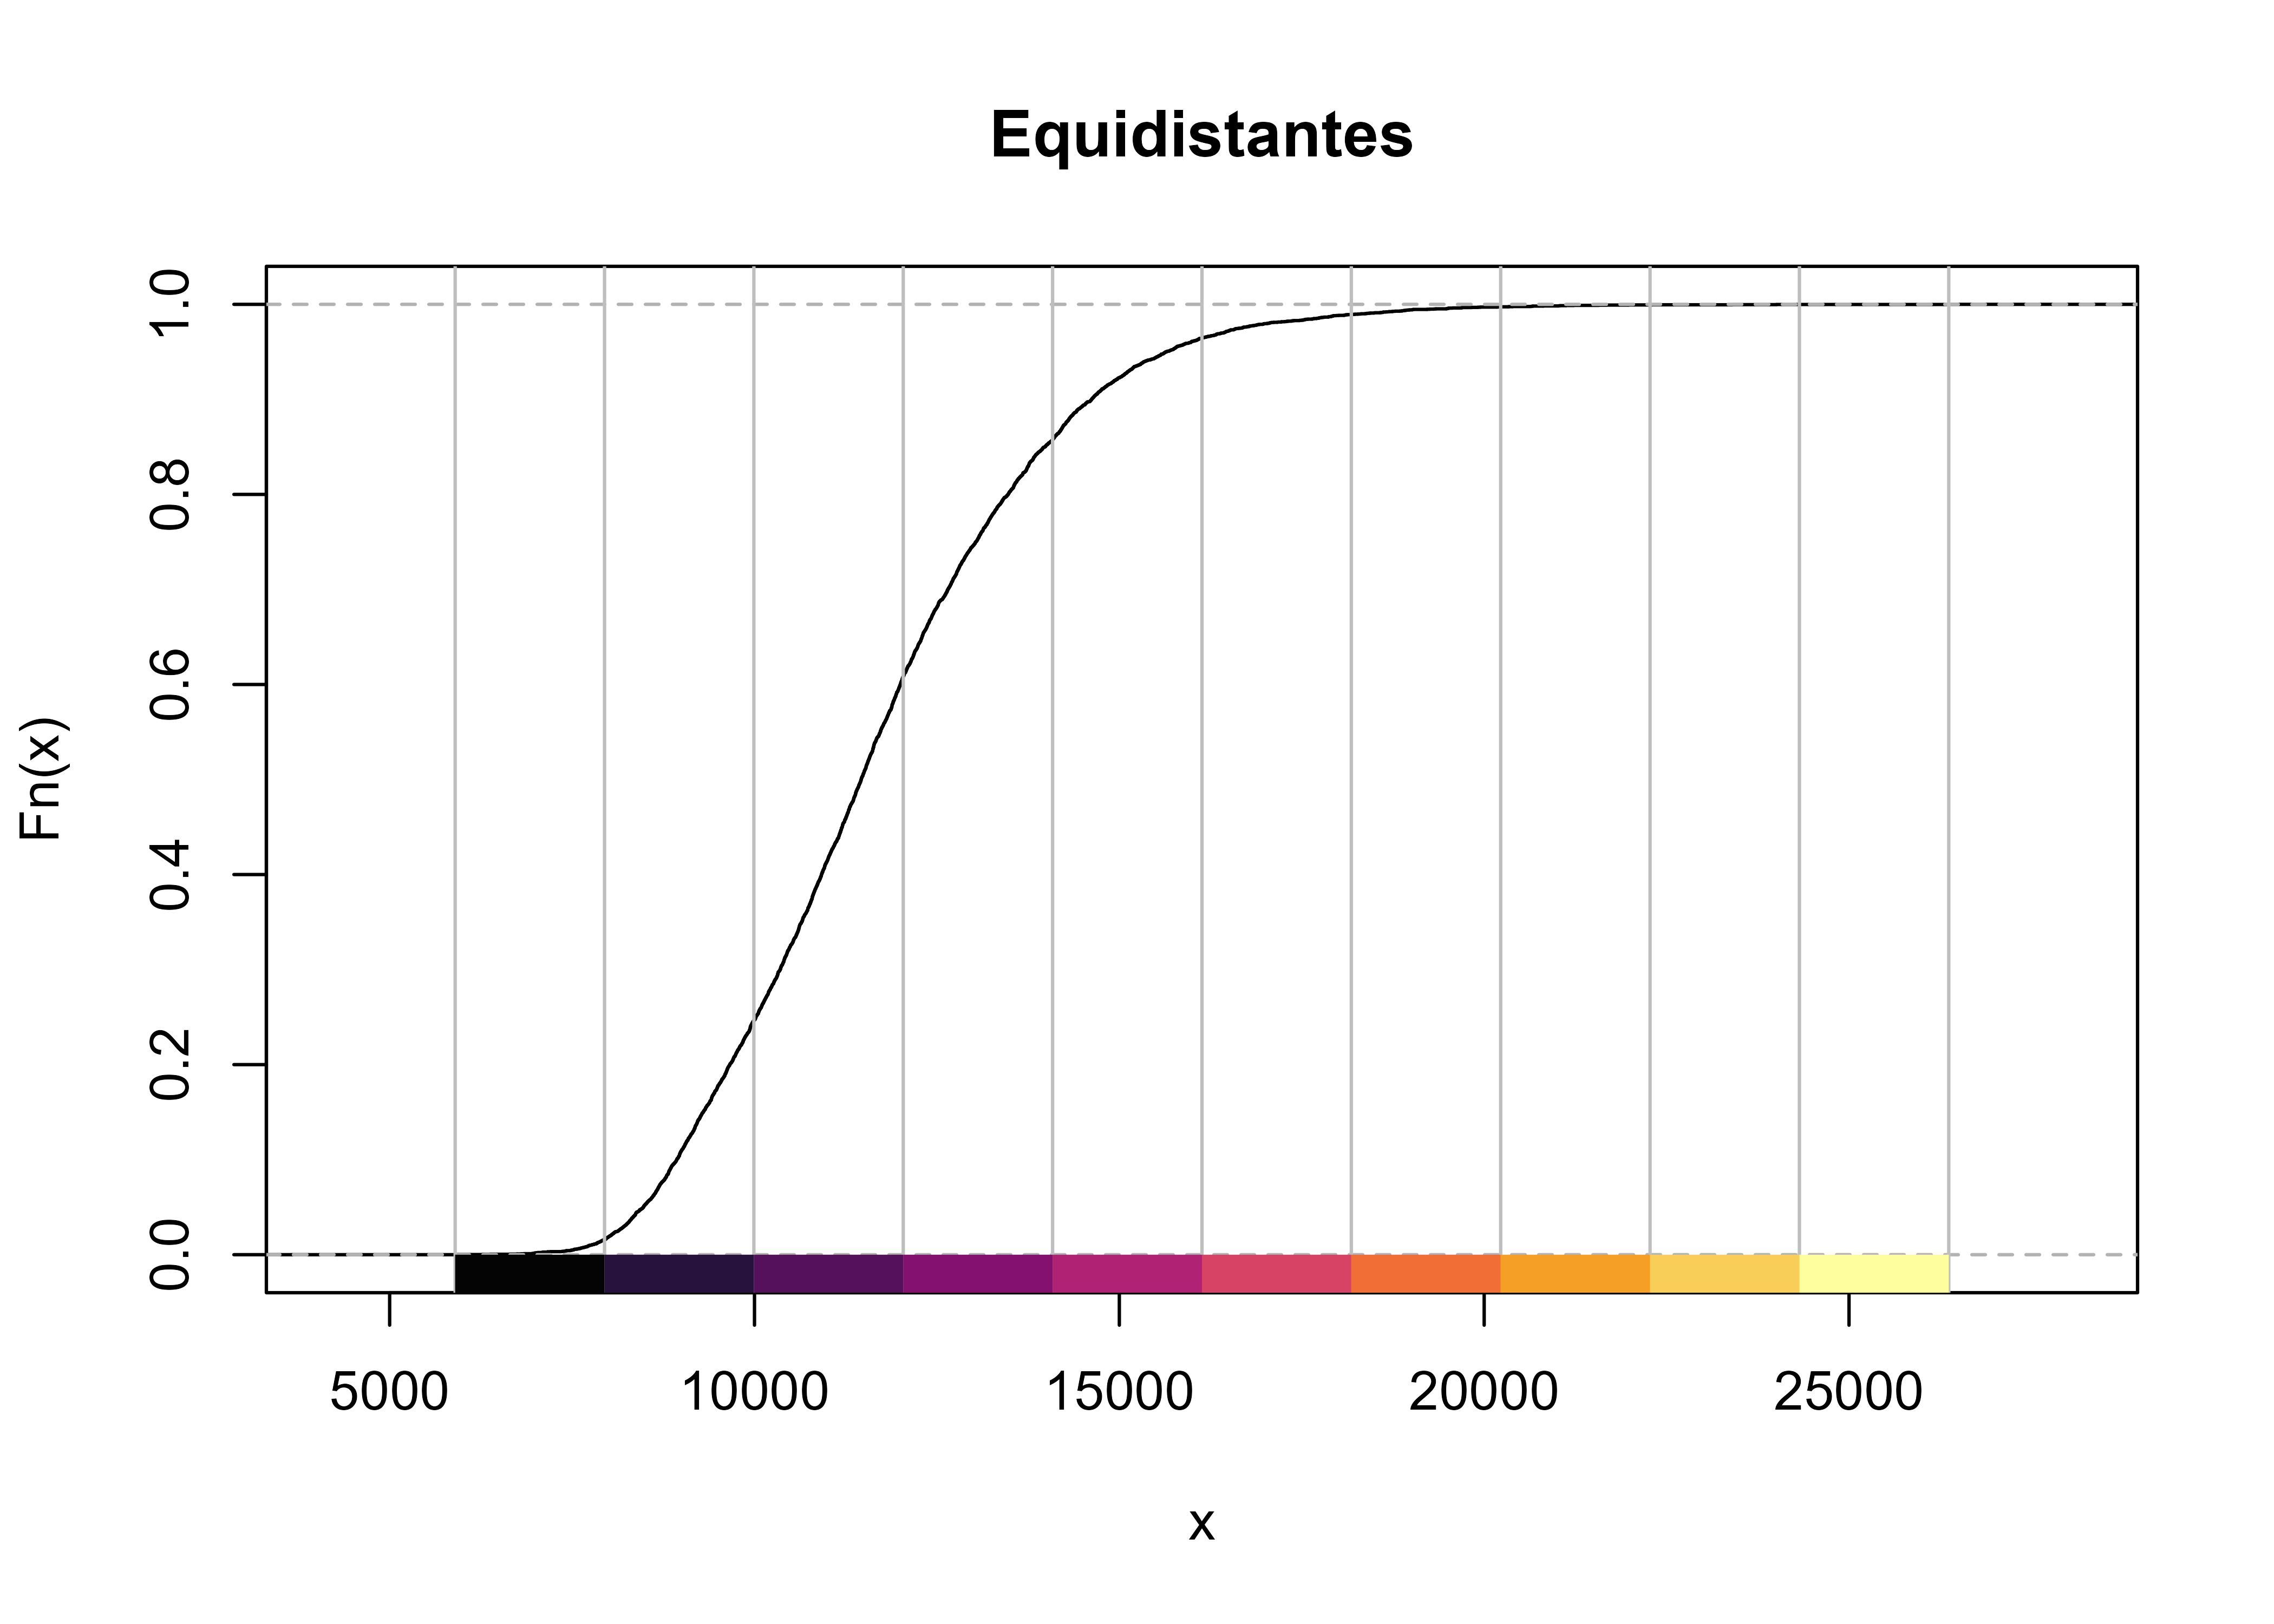
\includegraphics[width=0.6\linewidth]{_main_files/figure-latex/classint-2} \end{center}

\begin{Shaded}
\begin{Highlighting}[]

\NormalTok{fisher }\OtherTok{\textless{}{-}} \FunctionTok{classIntervals}\NormalTok{(munis\_renta\_clean}\SpecialCharTok{$}\StringTok{\textasciigrave{}}\AttributeTok{2019}\StringTok{\textasciigrave{}}\NormalTok{,}
  \AttributeTok{style =} \StringTok{"fisher"}\NormalTok{,}
  \CommentTok{\# Fuerzo para mejorar la comparación entre métodos}
  \AttributeTok{n =} \DecValTok{10}
\NormalTok{)}
\NormalTok{fisher}
\CommentTok{\#\textgreater{} style: fisher}
\CommentTok{\#\textgreater{}       [5898,8743)     [8743,9770.5)    [9770.5,10754)     [10754,11689) }
\CommentTok{\#\textgreater{}               505               904              1005              1159 }
\CommentTok{\#\textgreater{}     [11689,12668)     [12668,13803)   [13803,15222.5) [15222.5,17196.5) }
\CommentTok{\#\textgreater{}              1032               874               651               305 }
\CommentTok{\#\textgreater{} [17196.5,20063.5)   [20063.5,26367] }
\CommentTok{\#\textgreater{}               103                19}
\FunctionTok{plot}\NormalTok{(fisher,}
  \AttributeTok{pal =} \FunctionTok{hcl.colors}\NormalTok{(}\DecValTok{20}\NormalTok{, }\StringTok{"Inferno"}\NormalTok{),}
  \AttributeTok{main =} \StringTok{"Fisher{-}Jenks"}
\NormalTok{)}
\end{Highlighting}
\end{Shaded}

\begin{center}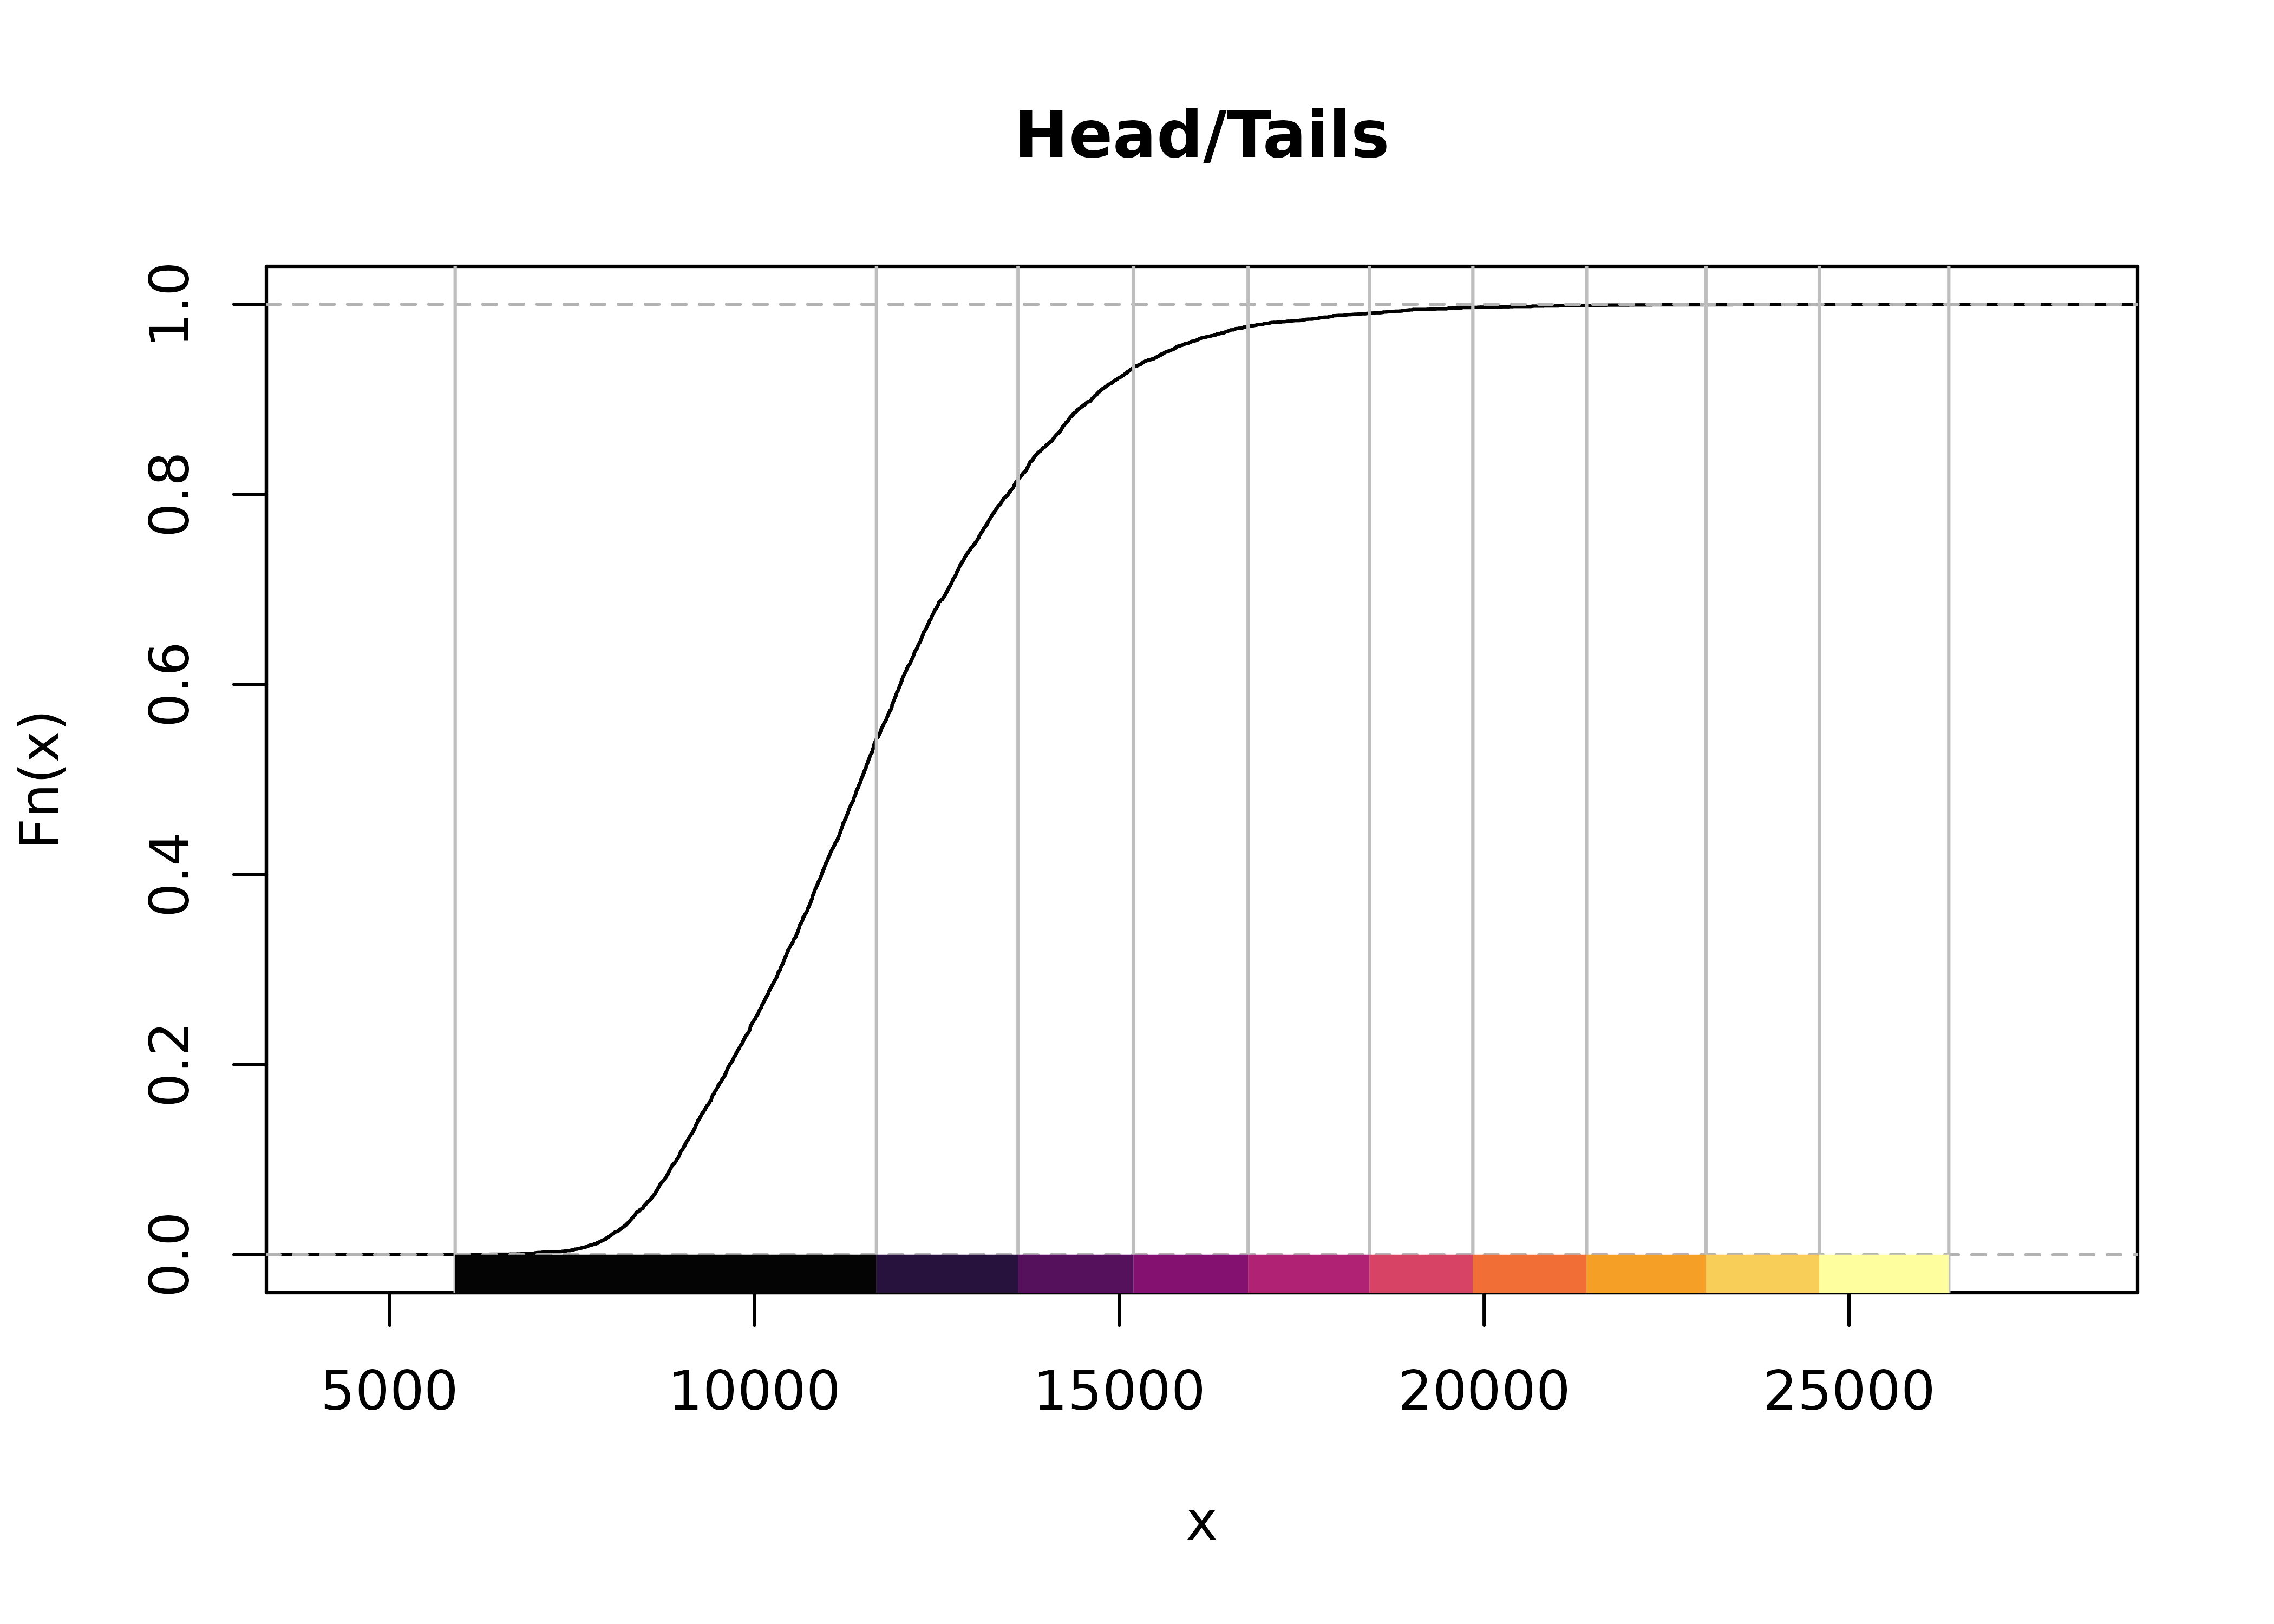
\includegraphics[width=0.6\linewidth]{_main_files/figure-latex/classint-3} \end{center}

Podemos observar lo siguiente:

\begin{itemize}
\item
  El último decil de renta se corresponde a un rango de entre 15.000 y 25.000
  €.
\item
  El método por deciles proporciona unos grupos con valores de renta muy
  parecidos entre sí en los valores medios. Esto es debido a la propia
  distribución de la variable.
\item
  El método de rangos equidistantes proporciona algunos grupos con un número
  muy reducido de municipios.
\item
  El método de Fisher-Jenks puede proporcionar unas clases con unos rangos más
  apropiados para los tramos altos de renta.
\end{itemize}

\emph{Tarea 8. Representar los mapas según las clases obtenidas}

Vamos ahora a realizar 3 mapas distintos, creando clases de renta según cada uno
de los métodos anteriormente mostrados.

\textbf{Deciles}

\begin{Shaded}
\begin{Highlighting}[]
\CommentTok{\# Extraigo los valores de corte}
\NormalTok{breaks\_d }\OtherTok{\textless{}{-}}\NormalTok{ deciles}\SpecialCharTok{$}\NormalTok{brks}

\CommentTok{\# Y creo unas etiquetas básicas para cada clase}
\CommentTok{\# Creo una función específica para crear etiquetas formateadas}
\NormalTok{label\_fun }\OtherTok{\textless{}{-}} \ControlFlowTok{function}\NormalTok{(x) \{}
\NormalTok{  l }\OtherTok{\textless{}{-}} \FunctionTok{length}\NormalTok{(x)}
\NormalTok{  eur }\OtherTok{\textless{}{-}} \FunctionTok{paste0}\NormalTok{(}\FunctionTok{prettyNum}\NormalTok{(}\FunctionTok{round}\NormalTok{(x, }\DecValTok{0}\NormalTok{),}
    \AttributeTok{decimal.mark =} \StringTok{","}\NormalTok{,}
    \AttributeTok{big.mark =} \StringTok{"."}
\NormalTok{  ), }\StringTok{" €"}\NormalTok{)}

\NormalTok{  labels }\OtherTok{\textless{}{-}} \FunctionTok{paste}\NormalTok{(eur[}\SpecialCharTok{{-}}\NormalTok{l], }\StringTok{"{-}"}\NormalTok{, eur[}\SpecialCharTok{{-}}\DecValTok{1}\NormalTok{])}
\NormalTok{  labels[}\DecValTok{1}\NormalTok{] }\OtherTok{\textless{}{-}} \FunctionTok{paste}\NormalTok{(}\StringTok{"\textless{}"}\NormalTok{, eur[}\DecValTok{1}\NormalTok{])}
\NormalTok{  labels[l }\SpecialCharTok{{-}} \DecValTok{1}\NormalTok{] }\OtherTok{\textless{}{-}} \FunctionTok{paste}\NormalTok{(}\StringTok{"\textgreater{}"}\NormalTok{, eur[l }\SpecialCharTok{{-}} \DecValTok{1}\NormalTok{])}
  \FunctionTok{return}\NormalTok{(labels)}
\NormalTok{\}}

\NormalTok{labels\_d }\OtherTok{\textless{}{-}} \FunctionTok{label\_fun}\NormalTok{(breaks\_d)}

\NormalTok{munis\_renta\_clean}\SpecialCharTok{$}\NormalTok{Deciles }\OtherTok{\textless{}{-}} \FunctionTok{cut}\NormalTok{(munis\_renta\_clean}\SpecialCharTok{$}\StringTok{\textasciigrave{}}\AttributeTok{2019}\StringTok{\textasciigrave{}}\NormalTok{,}
  \AttributeTok{breaks =}\NormalTok{ breaks\_d,}
  \AttributeTok{labels =}\NormalTok{ labels\_d,}
  \AttributeTok{include.lowest =} \ConstantTok{TRUE}
\NormalTok{)}

\FunctionTok{ggplot}\NormalTok{(munis\_renta\_clean) }\SpecialCharTok{+}
  \CommentTok{\# Cambiamos la variable que usamos para crear el mapa}
  \FunctionTok{geom\_sf}\NormalTok{(}\FunctionTok{aes}\NormalTok{(}\AttributeTok{fill =}\NormalTok{ Deciles), }\AttributeTok{color =} \ConstantTok{NA}\NormalTok{) }\SpecialCharTok{+}
  \CommentTok{\# Necesito cambiar el scale, ya no es continua}
  \FunctionTok{scale\_fill\_manual}\NormalTok{(}\AttributeTok{values =} \FunctionTok{hcl.colors}\NormalTok{(}\FunctionTok{length}\NormalTok{(labels\_d),}
    \StringTok{"Inferno"}\NormalTok{,}
    \AttributeTok{rev =} \ConstantTok{TRUE}
\NormalTok{  )) }\SpecialCharTok{+}
  \FunctionTok{theme\_minimal}\NormalTok{() }\SpecialCharTok{+}
  \FunctionTok{labs}\NormalTok{(}
    \AttributeTok{title =} \StringTok{"Renta neta media por persona"}\NormalTok{,}
    \AttributeTok{caption =} \StringTok{"Datos: INE"}
\NormalTok{  )}
\end{Highlighting}
\end{Shaded}

\begin{figure}

{\centering 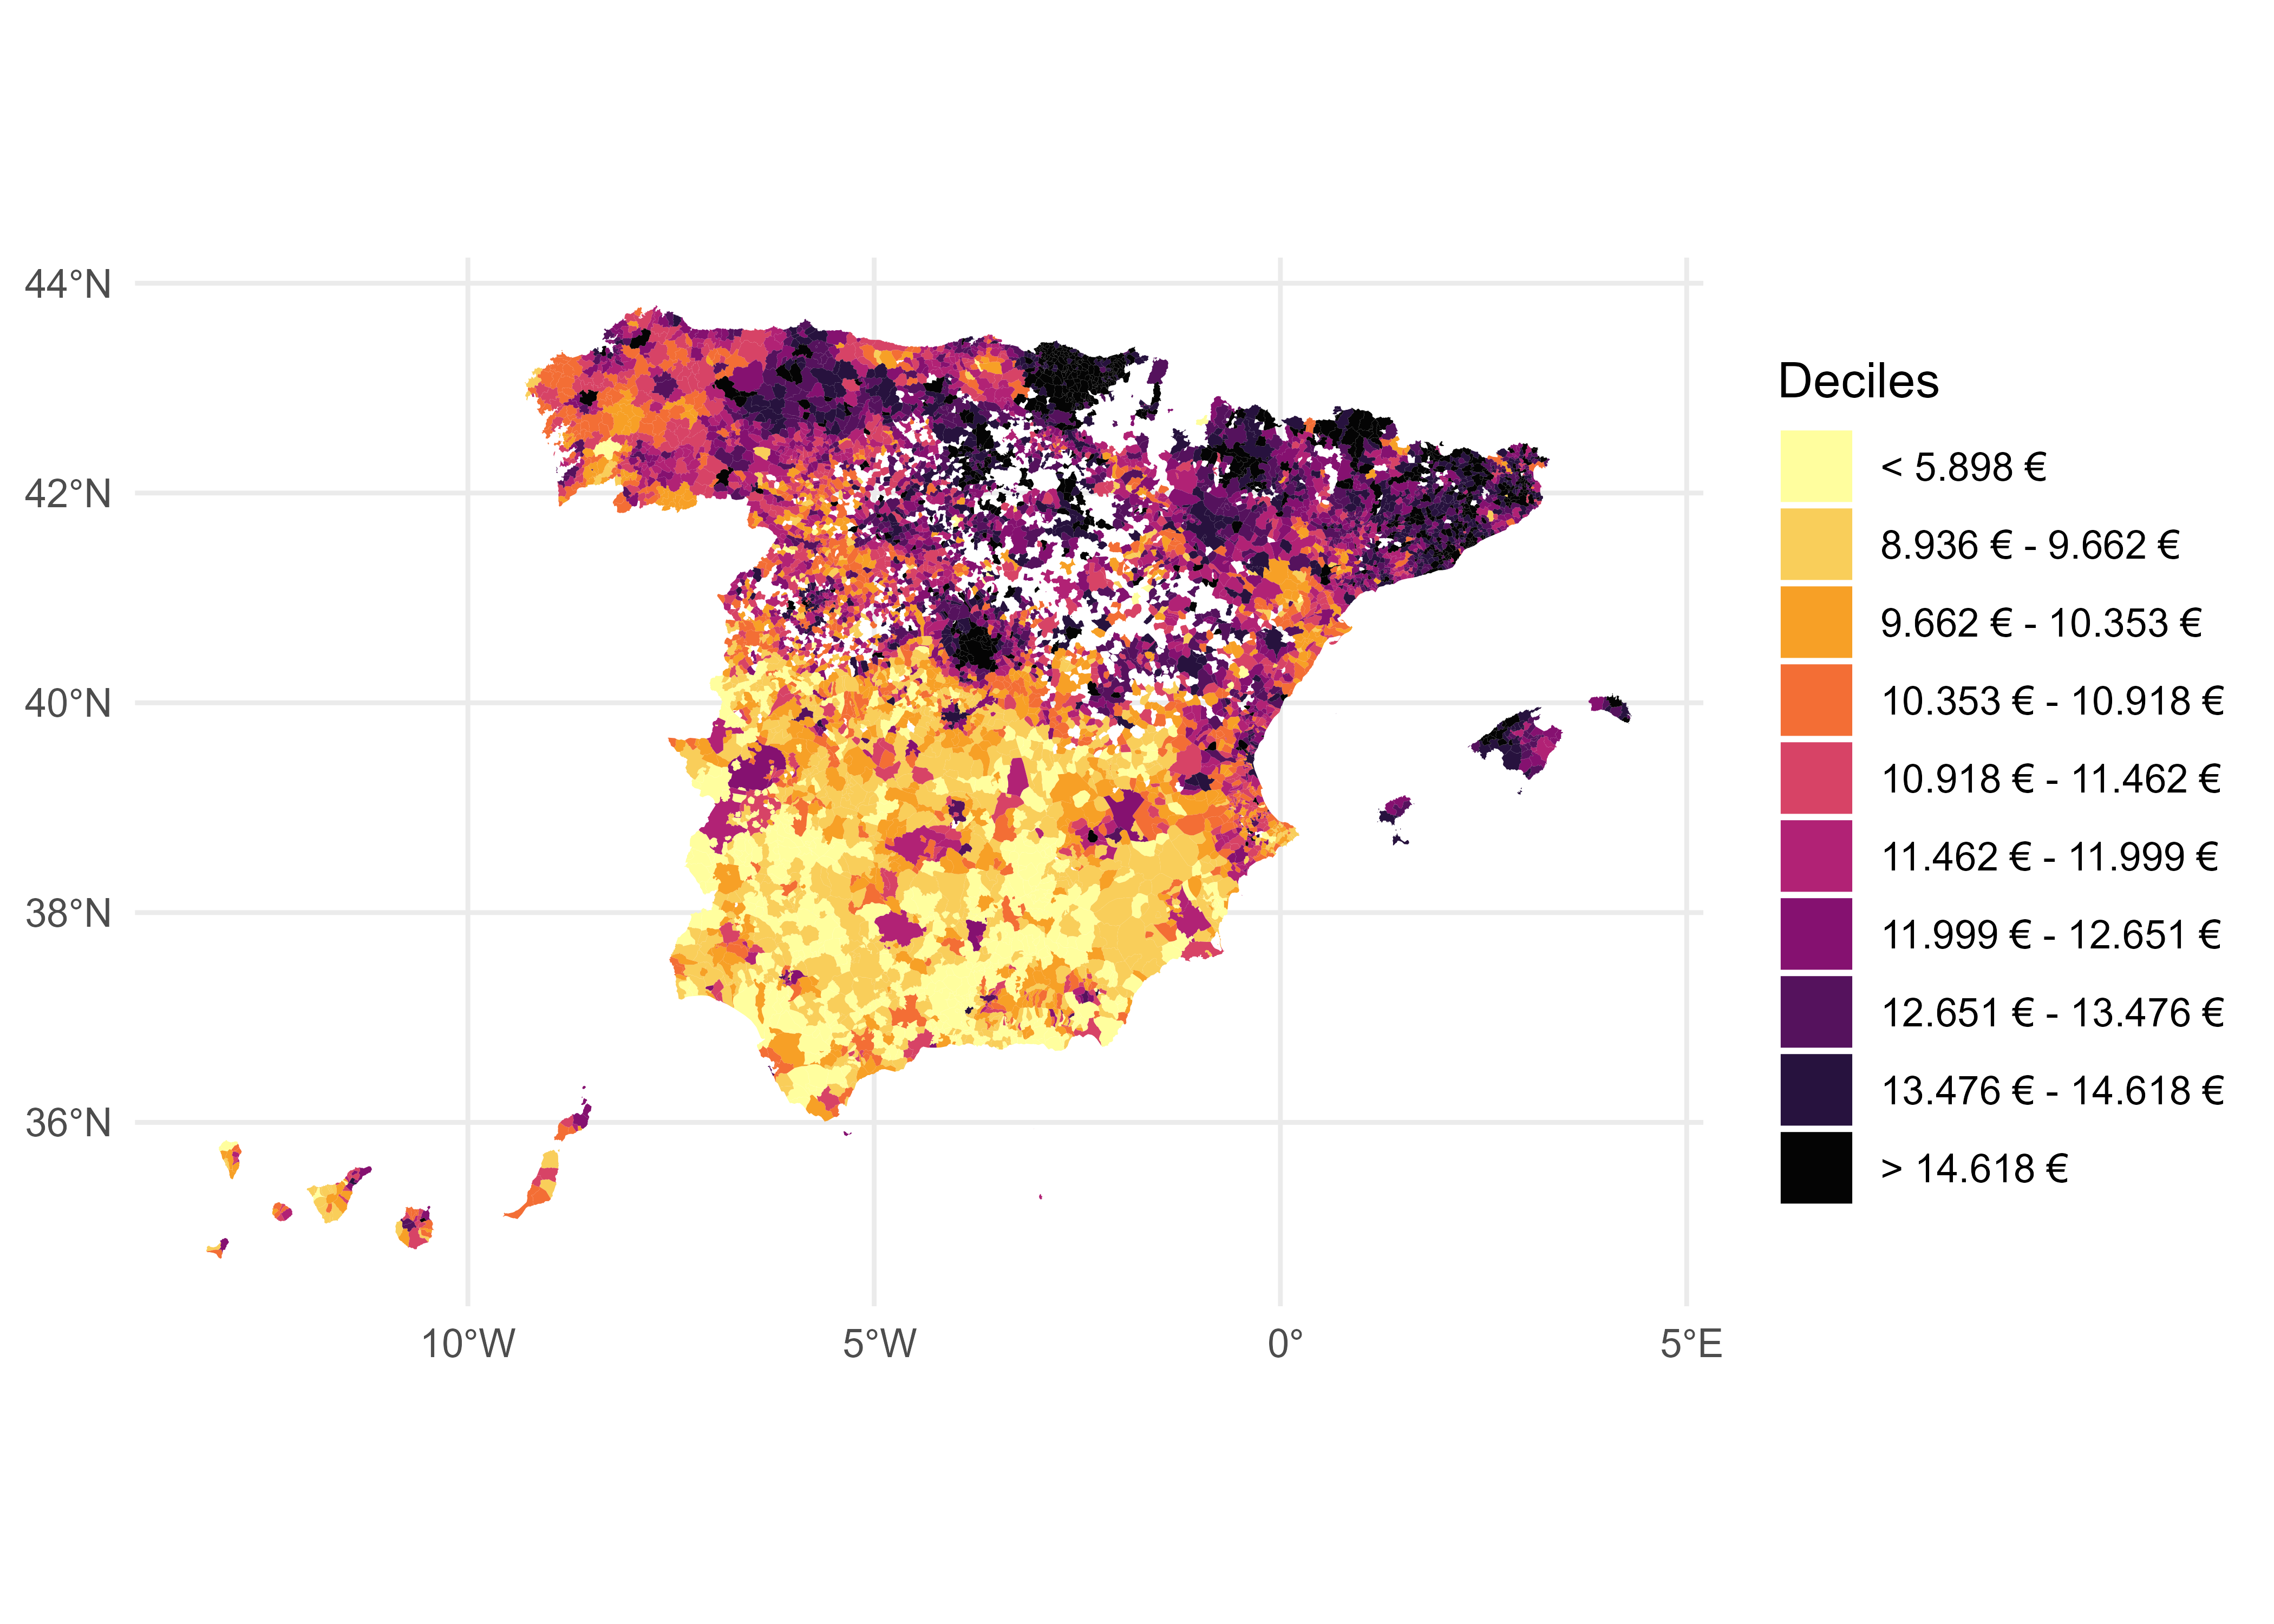
\includegraphics[width=0.6\linewidth]{_main_files/figure-latex/mapa-deciles-1} 

}

\caption{Mapa por deciles de renta}\label{fig:mapa-deciles}
\end{figure}

El mapa de la Fig. \ref{fig:mapa-deciles} ya nos permite observar patrones
geográficos, donde se ve una clara diferencia entre la Comunidades Autónomas del
Norte y las del Sur. Veamos una representación distina usando otras clases
diferentes:

\begin{Shaded}
\begin{Highlighting}[]

\NormalTok{breaks\_e }\OtherTok{\textless{}{-}}\NormalTok{ equal}\SpecialCharTok{$}\NormalTok{brks}
\NormalTok{labels\_e }\OtherTok{\textless{}{-}} \FunctionTok{label\_fun}\NormalTok{(breaks\_e)}

\NormalTok{munis\_renta\_clean}\SpecialCharTok{$}\NormalTok{Equal }\OtherTok{\textless{}{-}} \FunctionTok{cut}\NormalTok{(munis\_renta\_clean}\SpecialCharTok{$}\StringTok{\textasciigrave{}}\AttributeTok{2019}\StringTok{\textasciigrave{}}\NormalTok{,}
  \AttributeTok{breaks =}\NormalTok{ breaks\_e,}
  \AttributeTok{labels =}\NormalTok{ labels\_e,}
  \AttributeTok{include.lowest =} \ConstantTok{TRUE}
\NormalTok{)}

\FunctionTok{ggplot}\NormalTok{(munis\_renta\_clean) }\SpecialCharTok{+}
  \CommentTok{\# Cambiamos la variable que usamos para crear el mapa}
  \FunctionTok{geom\_sf}\NormalTok{(}\FunctionTok{aes}\NormalTok{(}\AttributeTok{fill =}\NormalTok{ Equal), }\AttributeTok{color =} \ConstantTok{NA}\NormalTok{) }\SpecialCharTok{+}
  \FunctionTok{scale\_fill\_manual}\NormalTok{(}\AttributeTok{values =} \FunctionTok{hcl.colors}\NormalTok{(}\FunctionTok{length}\NormalTok{(labels\_e),}
    \StringTok{"Inferno"}\NormalTok{,}
    \AttributeTok{rev =} \ConstantTok{TRUE}
\NormalTok{  )) }\SpecialCharTok{+}
  \FunctionTok{theme\_minimal}\NormalTok{() }\SpecialCharTok{+}
  \FunctionTok{labs}\NormalTok{(}
    \AttributeTok{title =} \StringTok{"Renta neta media por persona"}\NormalTok{,}
    \AttributeTok{caption =} \StringTok{"Datos: INE"}
\NormalTok{  )}
\end{Highlighting}
\end{Shaded}

\begin{figure}

{\centering 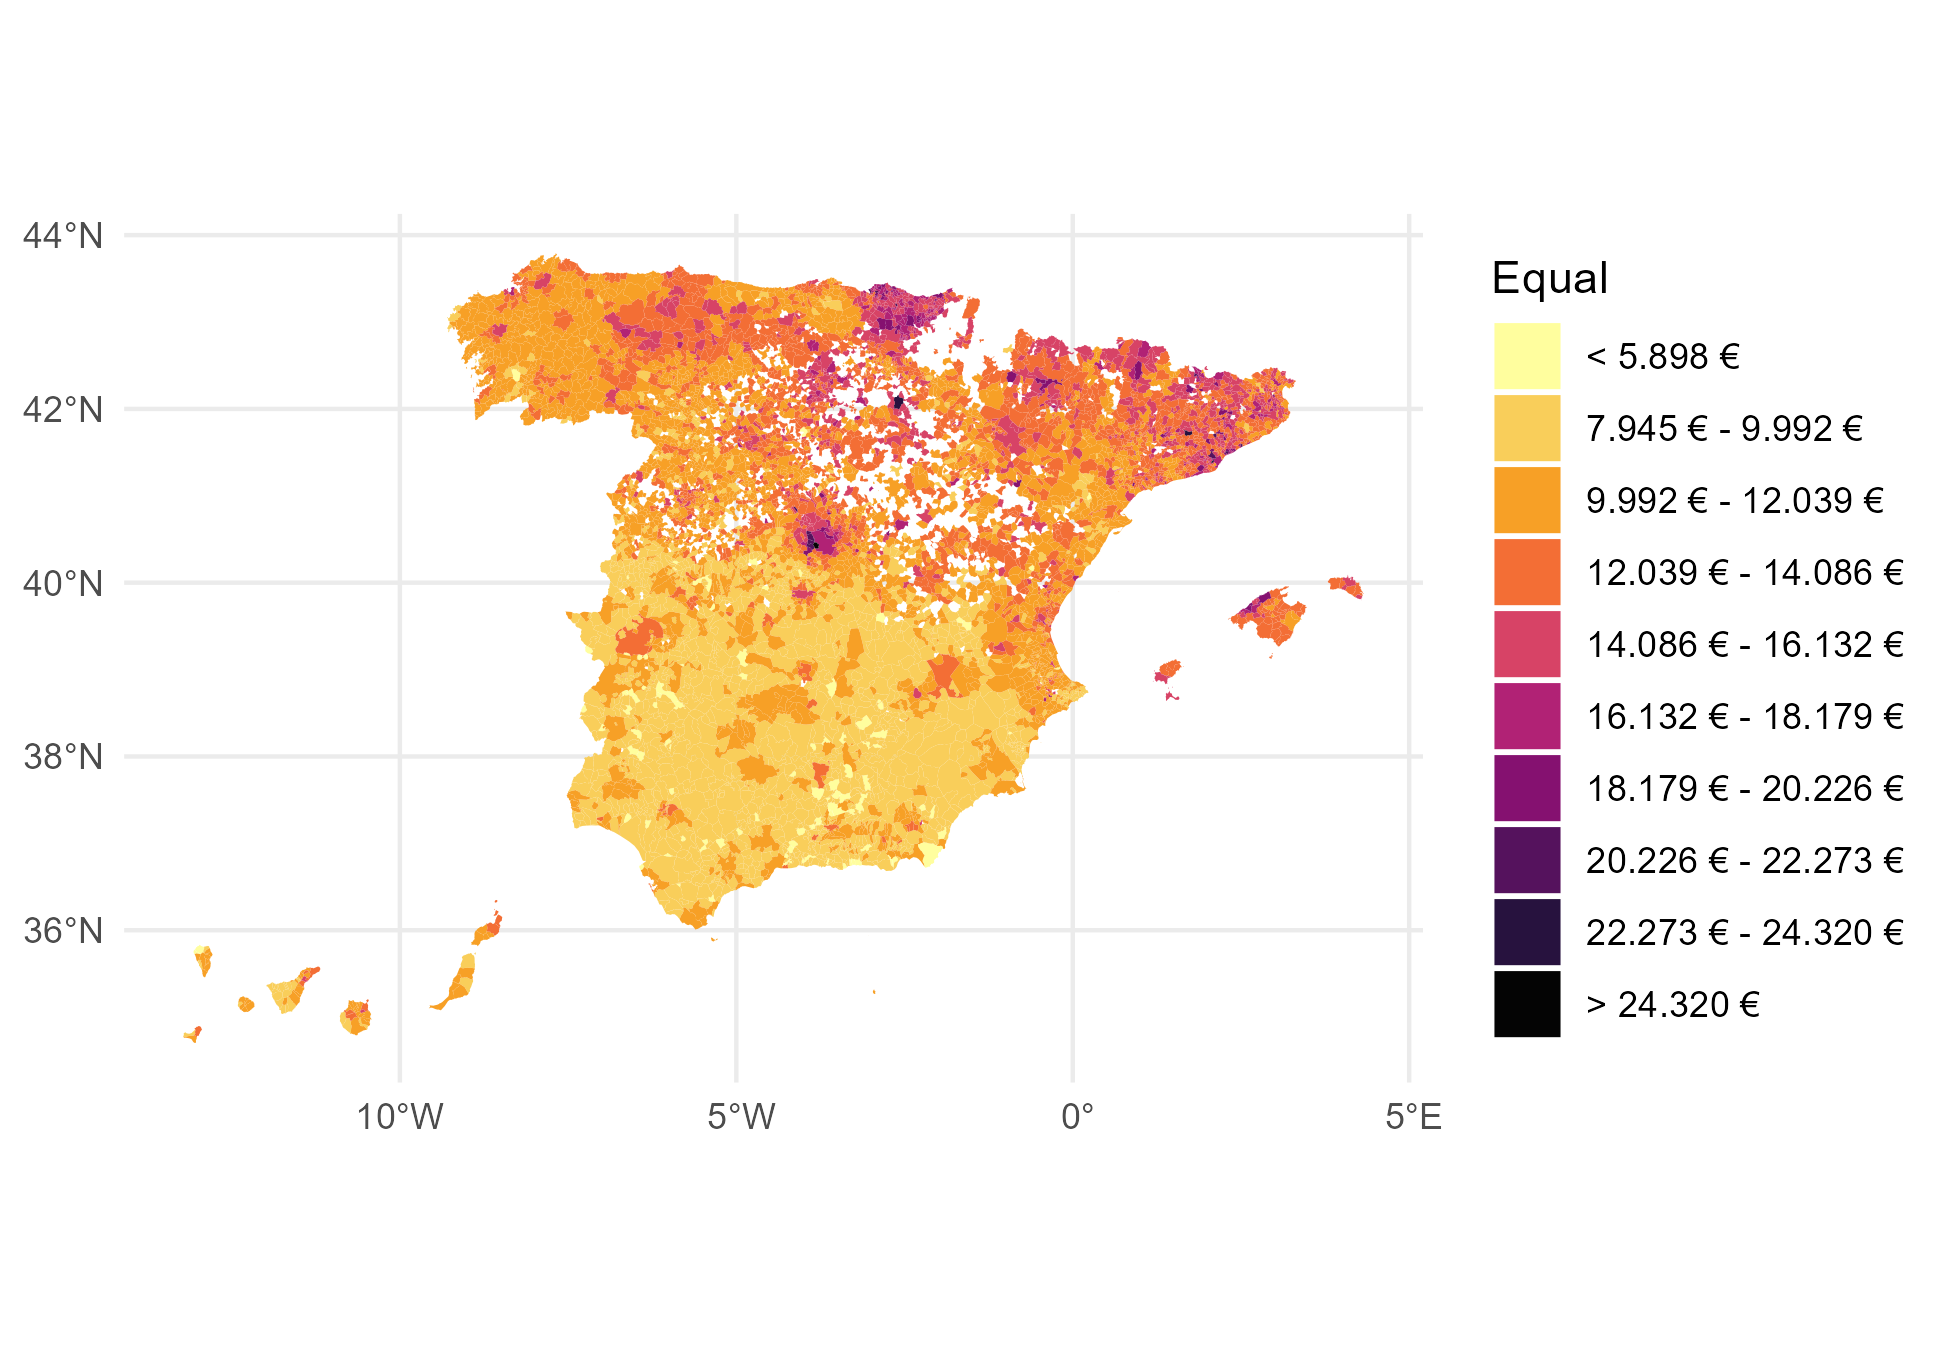
\includegraphics[width=0.6\linewidth]{_main_files/figure-latex/mapa-equal-1} 

}

\caption{Mapa por tramos de renta equidistantes}\label{fig:mapa-equal}
\end{figure}

El mapa de la Fig. \ref{fig:mapa-deciles}, sin embargo, se parece más al mapa
que hicimos con los datos sin clasificar, donde el peso visual se concentra más
bien en los municipios con rentas mucho más altas que el resto (por encimoa de
18.000 €).

Veamos el mismo mapa usando Fisher-Jenks:

\begin{Shaded}
\begin{Highlighting}[]

\NormalTok{breaks\_f }\OtherTok{\textless{}{-}}\NormalTok{ fisher}\SpecialCharTok{$}\NormalTok{brks}
\NormalTok{labels\_f }\OtherTok{\textless{}{-}} \FunctionTok{label\_fun}\NormalTok{(breaks\_f)}

\NormalTok{munis\_renta\_clean}\SpecialCharTok{$}\StringTok{\textasciigrave{}}\AttributeTok{Fisher{-}Jenks}\StringTok{\textasciigrave{}} \OtherTok{\textless{}{-}} \FunctionTok{cut}\NormalTok{(munis\_renta\_clean}\SpecialCharTok{$}\StringTok{\textasciigrave{}}\AttributeTok{2019}\StringTok{\textasciigrave{}}\NormalTok{,}
  \AttributeTok{breaks =}\NormalTok{ breaks\_f,}
  \AttributeTok{labels =}\NormalTok{ labels\_f,}
  \AttributeTok{include.lowest =} \ConstantTok{TRUE}
\NormalTok{)}

\FunctionTok{ggplot}\NormalTok{(munis\_renta\_clean) }\SpecialCharTok{+}
  \CommentTok{\# Cambiamos la variable que usamos para crear el mapa}
  \FunctionTok{geom\_sf}\NormalTok{(}\FunctionTok{aes}\NormalTok{(}\AttributeTok{fill =} \StringTok{\textasciigrave{}}\AttributeTok{Fisher{-}Jenks}\StringTok{\textasciigrave{}}\NormalTok{), }\AttributeTok{color =} \ConstantTok{NA}\NormalTok{) }\SpecialCharTok{+}
  \FunctionTok{scale\_fill\_manual}\NormalTok{(}\AttributeTok{values =} \FunctionTok{hcl.colors}\NormalTok{(}\FunctionTok{length}\NormalTok{(labels\_f),}
    \StringTok{"Inferno"}\NormalTok{,}
    \AttributeTok{rev =} \ConstantTok{TRUE}
\NormalTok{  )) }\SpecialCharTok{+}
  \FunctionTok{theme\_minimal}\NormalTok{() }\SpecialCharTok{+}
  \FunctionTok{labs}\NormalTok{(}
    \AttributeTok{title =} \StringTok{"Renta neta media por persona"}\NormalTok{,}
    \AttributeTok{caption =} \StringTok{"Datos: INE"}
\NormalTok{  )}
\end{Highlighting}
\end{Shaded}

\begin{figure}

{\centering 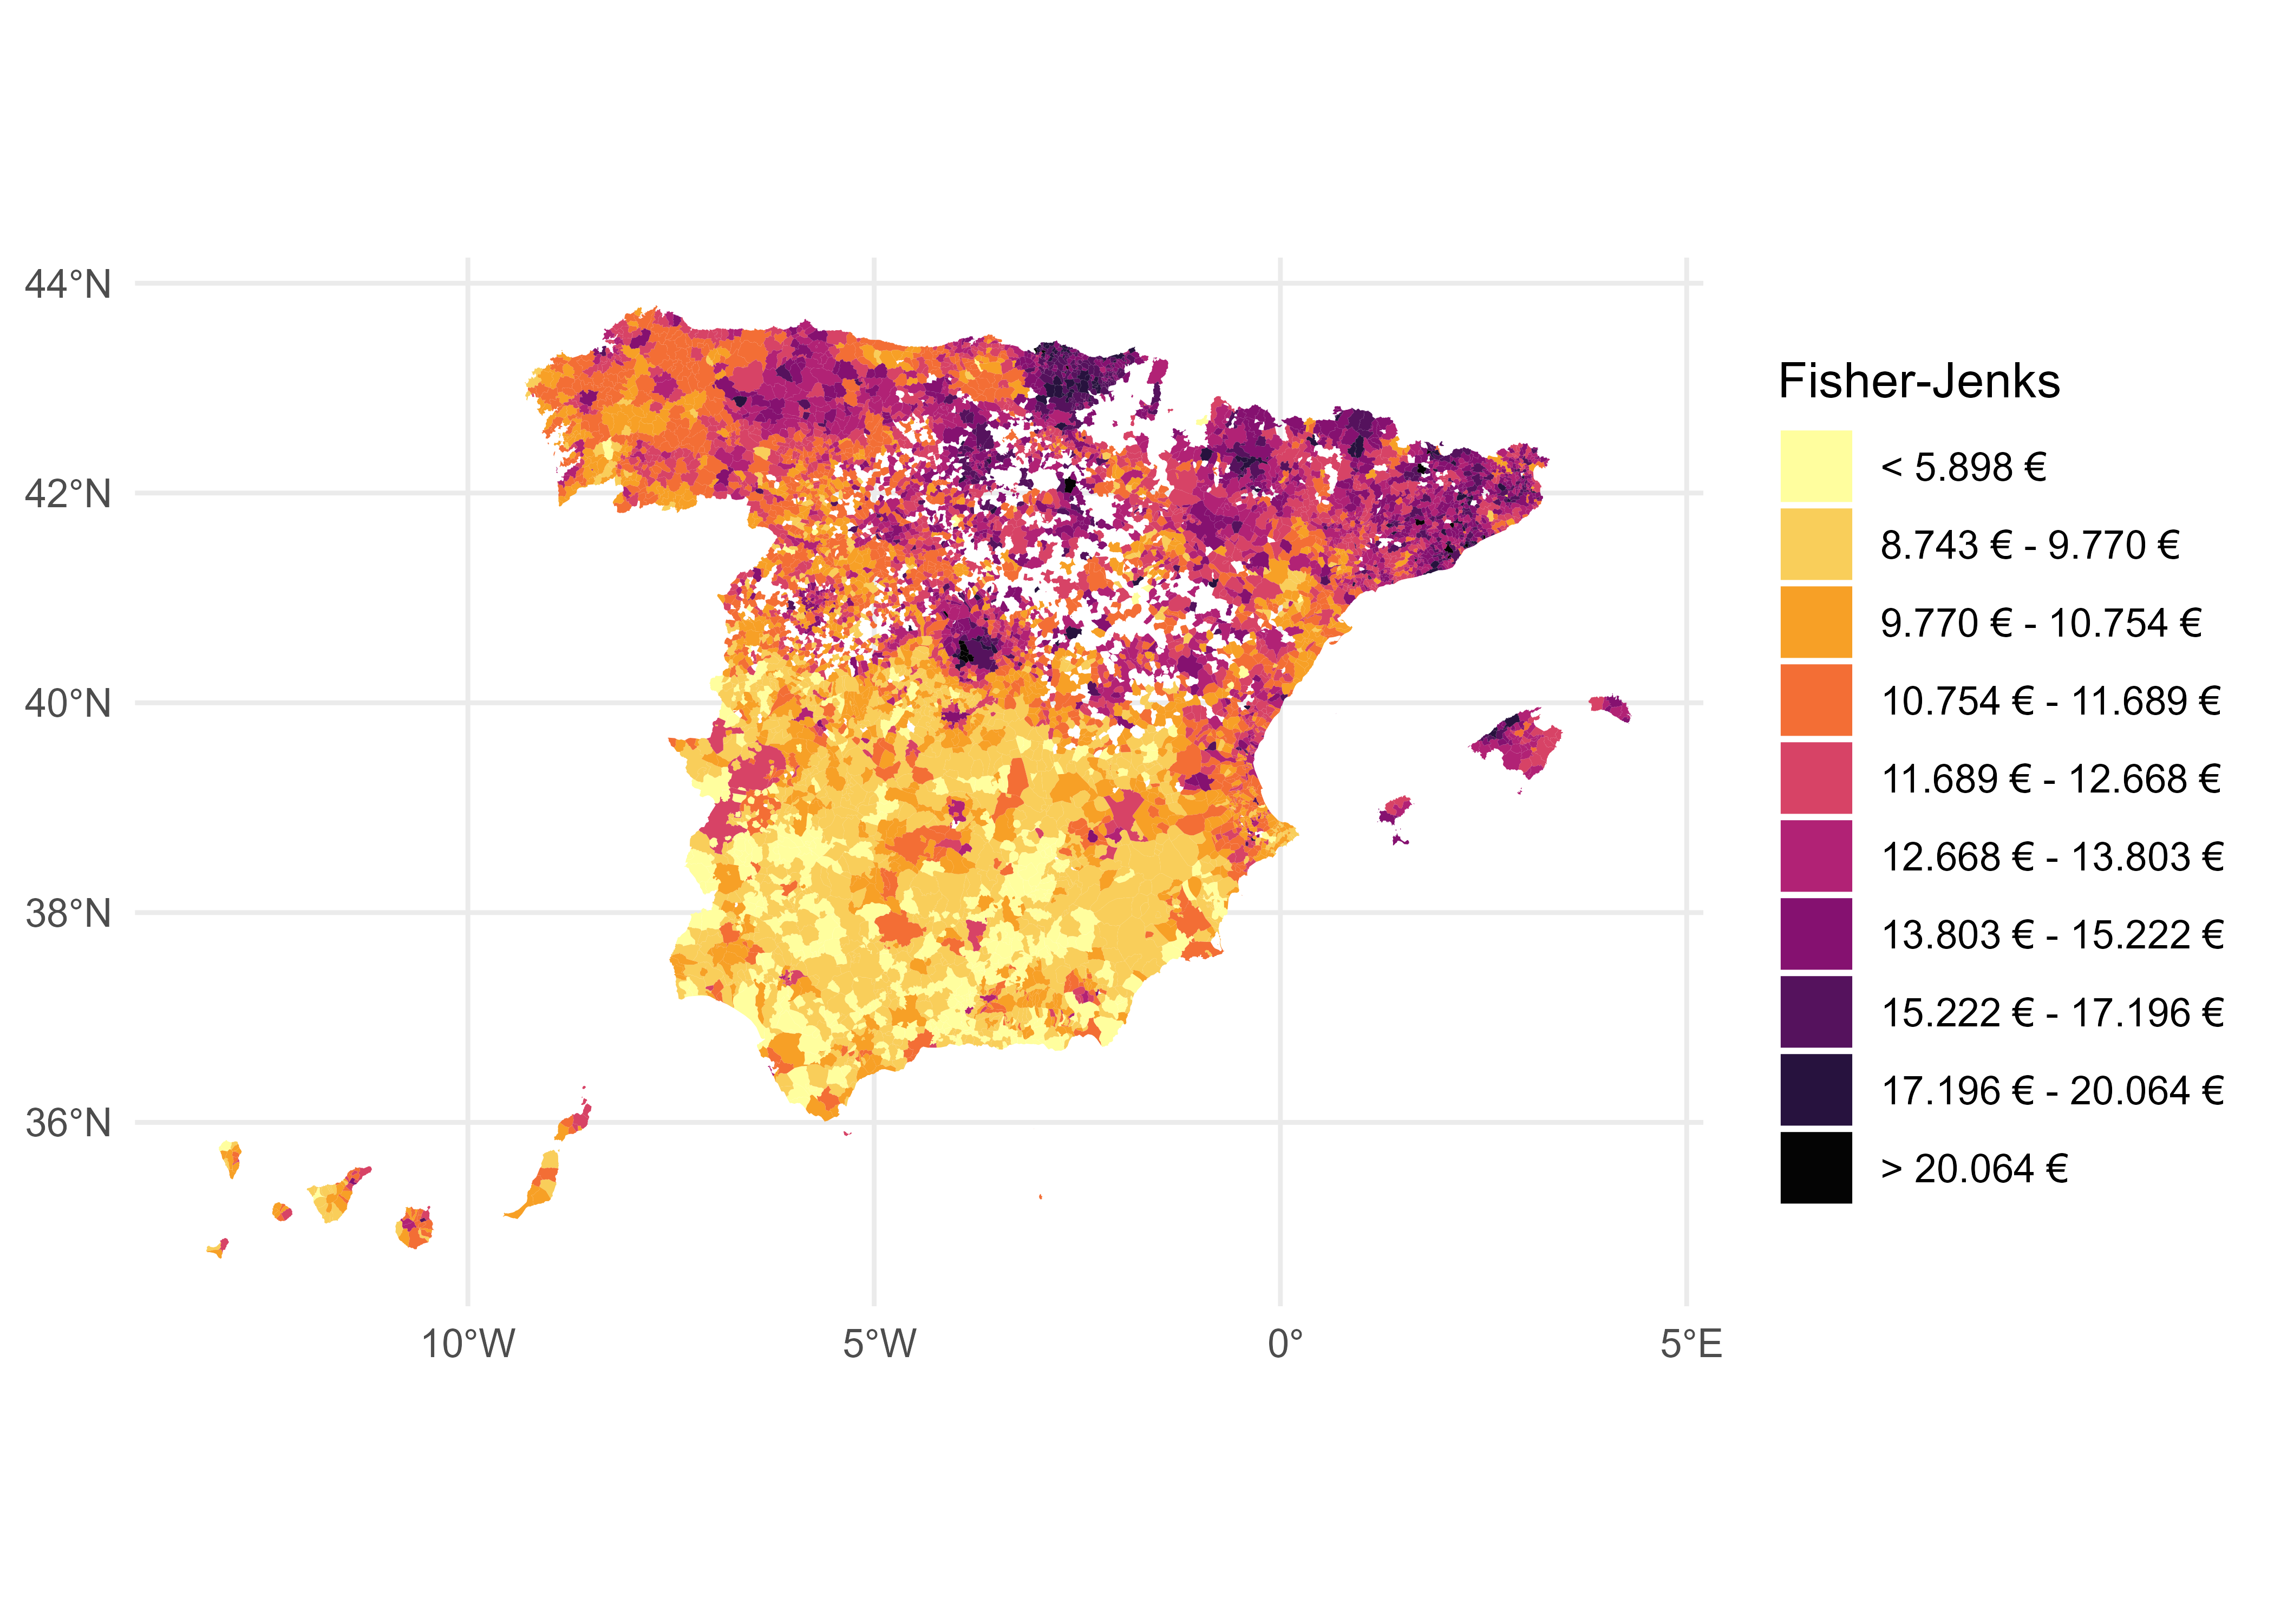
\includegraphics[width=0.6\linewidth]{_main_files/figure-latex/mapa-fisher-1} 

}

\caption{Mapa por tramos según Fisher-Jenks}\label{fig:mapa-fisher}
\end{figure}

En el mapa de la Fig. \ref{fig:mapa-deciles} se puede observar de una manera
más clara un cluster adicional de renta en la zona de Asturias y el norte de
León. Además, gracias a la escala de colores puede intuirse que este clúster de
renta no presenta valores tan altos como los observados en País Vasco o Madrid.

En conclusión, en el momento de realizar una visualización de datos es
importante conocer el dato a representar, así como entender algunas propiedades
básicas de la distribución subyacente. También hemos podido observar que hay
ciertas decisiones estéticas (datos continuos vs.~agrupados, escala de colores)
que tienen una influencia significativa en cómo se percibe la información
representada. Es responsabilidad del creador de la visualización el conocer
todos estos factores y aplicarlos de manera conveniente.

\textbf{Q4: Tenemos un mapa de los mismos datos pero la información se presenta de
manera sesgada, ¿puedes identificar los motivos?}

\begin{figure}

{\centering 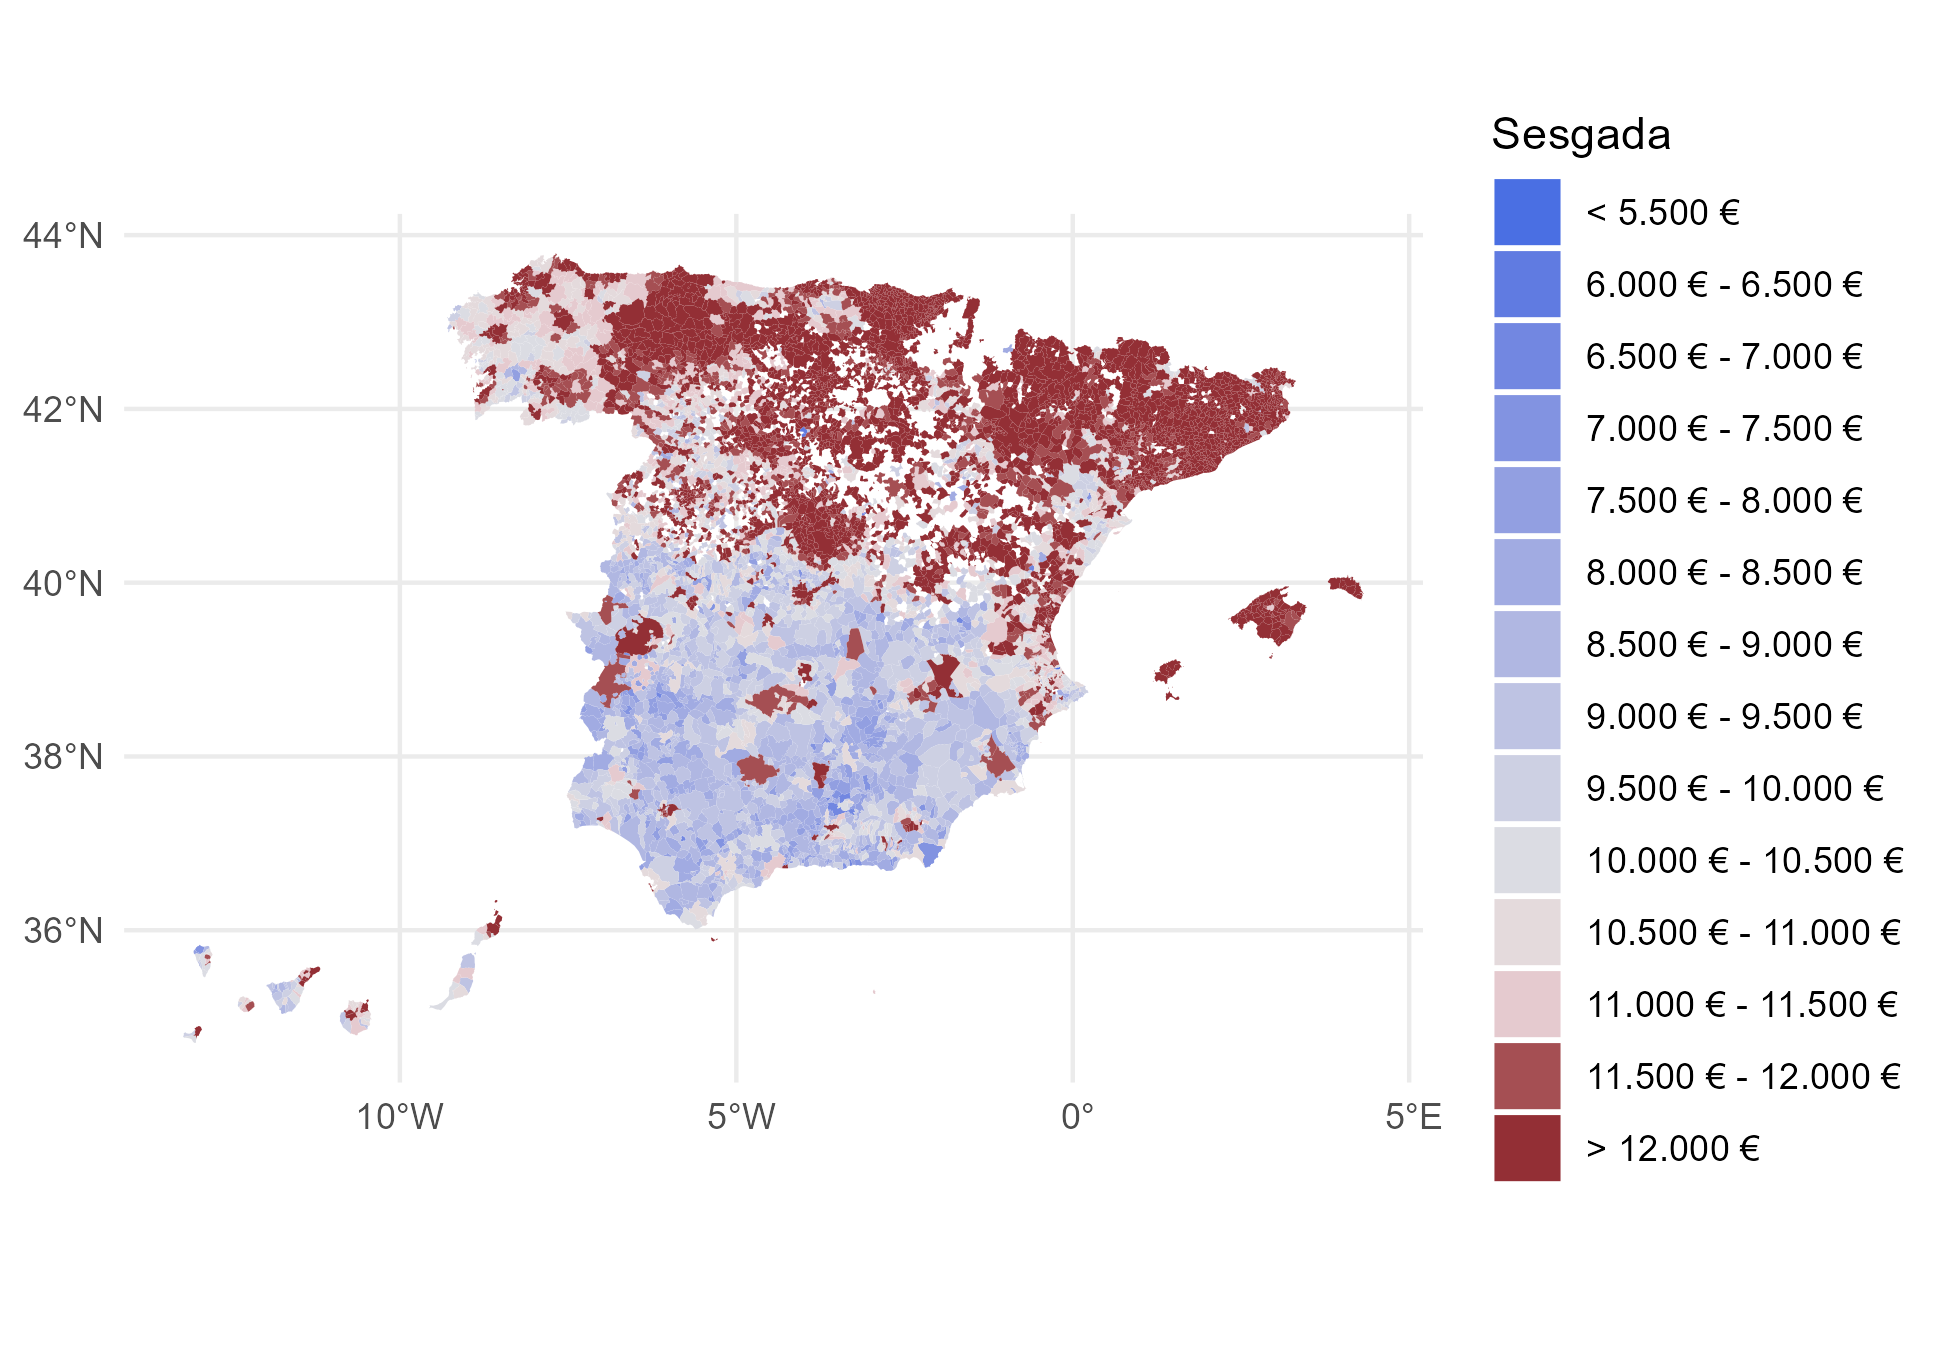
\includegraphics[width=0.6\linewidth]{_main_files/figure-latex/trucado-1} 

}

\caption{Ejemplo de visualización sesgada}\label{fig:trucado}
\end{figure}

En el mapa de la Fig. \ref{fig:trucado} parece que la renta per cápita de las
comunidades del norte es desproporcionadamente superior a las del sur. Resumimos
aquí los sesgos introducidos en el mapa:

\begin{itemize}
\item
  En primer lugar, se han creado un elevado número de grupos en las zonas de
  rentas bajas. De esta manera, la escala del mapa parece estar muy
  fragmentada, sin embargo muchos de esos grupos apenas contienen municipios.
  A modo de ejemplo, los primeros cuatro grupos únicamente contienen 32
  municipios.
\item
  Los grupos no se adaptan a la distribución subyacente de los datos. La
  mediana de los datos (11.462 €) estaría situada en la antepenúltima clase,
  de manera que los dos grupos de mayor renta contienen el 50\% de los
  municipios.
\item
  Además, la escala de color se ha manipulado, de manera que los grupos de
  mayores renta destaquen más que el resto de manera notoria.
\end{itemize}

\hypertarget{anuxe1lisis-de-patrones-de-puntos}{%
\section{Análisis de patrones de puntos}\label{anuxe1lisis-de-patrones-de-puntos}}

Las técnicas de análisis de patrones de puntos analizan la distribución de
eventos geolocalizados que surgen al azar. La diferencia fundamental con otros
análisis que comprenden también el uso de localizaciones (como las temperaturas
mínimas medidas por estaciones meteorológicas) es que en este caso los puntos
representan eventos conocidos y aleatorios (por ejemplo, los crímenes ocurridos
en una ciudad, accidentes de tráfico o incendios en una región). A diferencia de
otros eventos, como el ejemplo de las temperaturas mínimas, la ausencia de datos
no se debe a la ausencia de medición (e.g.~no existe una estación meteorológica
en ese lugar), si no a que no se ha producido el evento en dicha localización.

\textbf{Objetivo de aprendizaje}:

El alumno debe ser capaz de conocer los datos de tipo patrones de punto,
identificarlos y representarlos adecuadamente.

\emph{Tarea 1: Abrimos RStudio}

El presente análisis se va a realizar empleando RStudio, por lo que empezaremos
abriendo el programa y creando un nuevo script de R en \emph{Proyecto\textgreater File\textgreater New File\textgreater R
script}.

\emph{Tarea 2: Importamos y describimos los datos objeto de estudio}

El primer paso consiste en importar la base de datos de crímenes en la ciudad de
Valencia. El archivo está en formato csv, por lo que usaremos el paquete \texttt{readr}
para importar los datos:

\begin{Shaded}
\begin{Highlighting}[]
\FunctionTok{library}\NormalTok{(readr)}
\FunctionTok{library}\NormalTok{(dplyr)}

\CommentTok{\# En este caso el archivo está en la carpeta "data" de nuestro proyecto}
\NormalTok{crimen }\OtherTok{\textless{}{-}} \FunctionTok{read\_csv}\NormalTok{(}\StringTok{"data/crime{-}data{-}Valencia.csv"}\NormalTok{)}


\FunctionTok{summary}\NormalTok{(crimen)}
\CommentTok{\#\textgreater{}    crime\_id          crime\_date         crime\_time        crime\_type       }
\CommentTok{\#\textgreater{}  Length:90247       Length:90247       Length:90247      Length:90247      }
\CommentTok{\#\textgreater{}  Class :character   Class :character   Class1:hms        Class :character  }
\CommentTok{\#\textgreater{}  Mode  :character   Mode  :character   Class2:difftime   Mode  :character  }
\CommentTok{\#\textgreater{}                                        Mode  :numeric                      }
\CommentTok{\#\textgreater{}                                                                            }
\CommentTok{\#\textgreater{}                                                                            }
\CommentTok{\#\textgreater{}      muni                year          month             week      }
\CommentTok{\#\textgreater{}  Length:90247       Min.   :2010   Min.   : 1.000   Min.   : 1.00  }
\CommentTok{\#\textgreater{}  Class :character   1st Qu.:2013   1st Qu.: 4.000   1st Qu.:14.00  }
\CommentTok{\#\textgreater{}  Mode  :character   Median :2016   Median : 7.000   Median :27.00  }
\CommentTok{\#\textgreater{}                     Mean   :2015   Mean   : 6.537   Mean   :26.65  }
\CommentTok{\#\textgreater{}                     3rd Qu.:2018   3rd Qu.: 9.000   3rd Qu.:38.00  }
\CommentTok{\#\textgreater{}                     Max.   :2020   Max.   :12.000   Max.   :53.00  }
\CommentTok{\#\textgreater{}       day           week\_day     week\_day\_name        crime\_hour   }
\CommentTok{\#\textgreater{}  Min.   :  1.0   Min.   :1.000   Length:90247       Min.   : 0.00  }
\CommentTok{\#\textgreater{}  1st Qu.: 96.0   1st Qu.:3.000   Class :character   1st Qu.: 5.00  }
\CommentTok{\#\textgreater{}  Median :187.0   Median :5.000   Mode  :character   Median :14.00  }
\CommentTok{\#\textgreater{}  Mean   :183.6   Mean   :4.323                      Mean   :12.52  }
\CommentTok{\#\textgreater{}  3rd Qu.:266.0   3rd Qu.:6.000                      3rd Qu.:19.00  }
\CommentTok{\#\textgreater{}  Max.   :366.0   Max.   :7.000                      Max.   :23.00  }
\CommentTok{\#\textgreater{}    crime\_lon         crime\_lat        atm\_dist          bank\_dist       }
\CommentTok{\#\textgreater{}  Min.   :{-}0.4296   Min.   :39.42   Min.   :   1.549   Min.   :   1.713  }
\CommentTok{\#\textgreater{}  1st Qu.:{-}0.3883   1st Qu.:39.46   1st Qu.: 380.535   1st Qu.: 133.908  }
\CommentTok{\#\textgreater{}  Median :{-}0.3749   Median :39.47   Median : 630.867   Median : 228.003  }
\CommentTok{\#\textgreater{}  Mean   :{-}0.3724   Mean   :39.47   Mean   : 790.228   Mean   : 305.315  }
\CommentTok{\#\textgreater{}  3rd Qu.:{-}0.3593   3rd Qu.:39.48   3rd Qu.: 986.897   3rd Qu.: 384.706  }
\CommentTok{\#\textgreater{}  Max.   :{-}0.3208   Max.   :39.53   Max.   :4838.847   Max.   :3411.537  }
\CommentTok{\#\textgreater{}     bar\_dist          cafe\_dist        industrial\_dist   market\_dist      }
\CommentTok{\#\textgreater{}  Min.   :   0.489   Min.   :   1.342   Min.   :   0.1   Min.   :   1.821  }
\CommentTok{\#\textgreater{}  1st Qu.: 149.879   1st Qu.: 133.274   1st Qu.: 268.4   1st Qu.: 487.874  }
\CommentTok{\#\textgreater{}  Median : 292.246   Median : 264.504   Median : 509.6   Median : 869.516  }
\CommentTok{\#\textgreater{}  Mean   : 392.072   Mean   : 360.275   Mean   : 675.2   Mean   :1008.414  }
\CommentTok{\#\textgreater{}  3rd Qu.: 507.701   3rd Qu.: 462.982   3rd Qu.: 909.9   3rd Qu.:1263.405  }
\CommentTok{\#\textgreater{}  Max.   :4352.380   Max.   :4237.915   Max.   :4703.9   Max.   :4855.407  }
\CommentTok{\#\textgreater{}  nightclub\_dist      police\_dist          pub\_dist        restaurant\_dist   }
\CommentTok{\#\textgreater{}  Min.   :   1.189   Min.   :   0.688   Min.   :   1.489   Min.   :   0.427  }
\CommentTok{\#\textgreater{}  1st Qu.: 468.164   1st Qu.: 455.810   1st Qu.: 190.150   1st Qu.:  73.401  }
\CommentTok{\#\textgreater{}  Median : 810.185   Median : 706.094   Median : 383.330   Median : 147.797  }
\CommentTok{\#\textgreater{}  Mean   : 930.501   Mean   : 875.246   Mean   : 496.472   Mean   : 223.875  }
\CommentTok{\#\textgreater{}  3rd Qu.:1256.269   3rd Qu.:1105.625   3rd Qu.: 665.599   3rd Qu.: 272.288  }
\CommentTok{\#\textgreater{}  Max.   :4700.567   Max.   :4765.745   Max.   :4168.869   Max.   :3746.536  }
\CommentTok{\#\textgreater{}    taxi\_dist           grid\_id         grid\_lon          grid\_lat    }
\CommentTok{\#\textgreater{}  Min.   :   2.441   Min.   :  8.0   Min.   :{-}0.4288   Min.   :39.42  }
\CommentTok{\#\textgreater{}  1st Qu.: 393.438   1st Qu.:173.0   1st Qu.:{-}0.3898   1st Qu.:39.46  }
\CommentTok{\#\textgreater{}  Median : 651.644   Median :215.0   Median :{-}0.3731   Median :39.47  }
\CommentTok{\#\textgreater{}  Mean   : 717.381   Mean   :210.8   Mean   :{-}0.3724   Mean   :39.47  }
\CommentTok{\#\textgreater{}  3rd Qu.: 931.083   3rd Qu.:248.0   3rd Qu.:{-}0.3620   3rd Qu.:39.48  }
\CommentTok{\#\textgreater{}  Max.   :4284.239   Max.   :398.0   Max.   :{-}0.3230   Max.   :39.53}
\end{Highlighting}
\end{Shaded}

\textbf{Q1: ¿Qué información contiene nuestros datos?}

Este archivo contiene en total
90.247 registros, y
proporciona 28 campos asociados a cada registro.

Entre los campos disponibles, destacamos los campos \texttt{crime\_lon} y \texttt{crime\_lat}:
Son las coordenadas en las que se produjo el crimen.

\textbf{Q2: ¿En qué CRS se encuentran las coordenadas?}

Si nos fijamos, las coordenadas parecen corresponder con longitudes y latitudes,
ya que como se explicó el rango posible de valores es \([-180, 180]\) (para
longitudes) y \([-90, 90]\) (para latitudes):

\begin{table}

\caption{\label{tab:coods-lonlat}Crímenes en Valencia; Coordenadas}
\centering
\begin{tabular}[t]{r|r}
\hline
crime\_lon & crime\_lat\\
\hline
-0.3826325 & 39.46332\\
\hline
-0.3906850 & 39.43517\\
\hline
-0.3747971 & 39.47927\\
\hline
-0.3992082 & 39.47982\\
\hline
-0.3596011 & 39.46740\\
\hline
-0.3552423 & 39.47461\\
\hline
\end{tabular}
\end{table}

Por lo tanto, podemos convertir la tabla en un objecto \texttt{sf} teniendo en cuenta
esta información. A modo de recordatorio, el CRS correspondiente a coordenadas
geográficas longitud/latitud es \textbf{EPSG:4326}.

\begin{Shaded}
\begin{Highlighting}[]

\FunctionTok{library}\NormalTok{(sf)}
\CommentTok{\# Objeto sf sin CRS}

\NormalTok{crimen\_sf }\OtherTok{\textless{}{-}} \FunctionTok{st\_as\_sf}\NormalTok{(}
\NormalTok{  crimen,}
  \AttributeTok{coords =} \FunctionTok{c}\NormalTok{(}
    \StringTok{"crime\_lon"}\NormalTok{,}
    \StringTok{"crime\_lat"}
\NormalTok{  ),}
  \AttributeTok{crs =} \FunctionTok{st\_crs}\NormalTok{(}\DecValTok{4326}\NormalTok{)}
\NormalTok{)}

\CommentTok{\# Comprobamos con un mapa base}

\FunctionTok{library}\NormalTok{(mapSpain)}
\FunctionTok{library}\NormalTok{(ggplot2)}

\CommentTok{\# Usamos imagen como mapa de fondo}
\NormalTok{tile }\OtherTok{\textless{}{-}} \FunctionTok{esp\_getTiles}\NormalTok{(crimen\_sf, }\StringTok{"IDErioja"}\NormalTok{,}
  \AttributeTok{zoommin =} \DecValTok{1}\NormalTok{,}
  \AttributeTok{crop =} \ConstantTok{TRUE}
\NormalTok{)}

\FunctionTok{ggplot}\NormalTok{() }\SpecialCharTok{+}
  \FunctionTok{layer\_spatraster}\NormalTok{(tile) }\SpecialCharTok{+}
  \FunctionTok{geom\_sf}\NormalTok{(}
    \AttributeTok{data =}\NormalTok{ crimen\_sf,}
    \AttributeTok{col =} \StringTok{"blue"}\NormalTok{,}
    \AttributeTok{size =} \FloatTok{0.3}\NormalTok{,}
    \AttributeTok{alpha =} \FloatTok{0.3}
\NormalTok{  )}
\end{Highlighting}
\end{Shaded}

\begin{figure}

{\centering 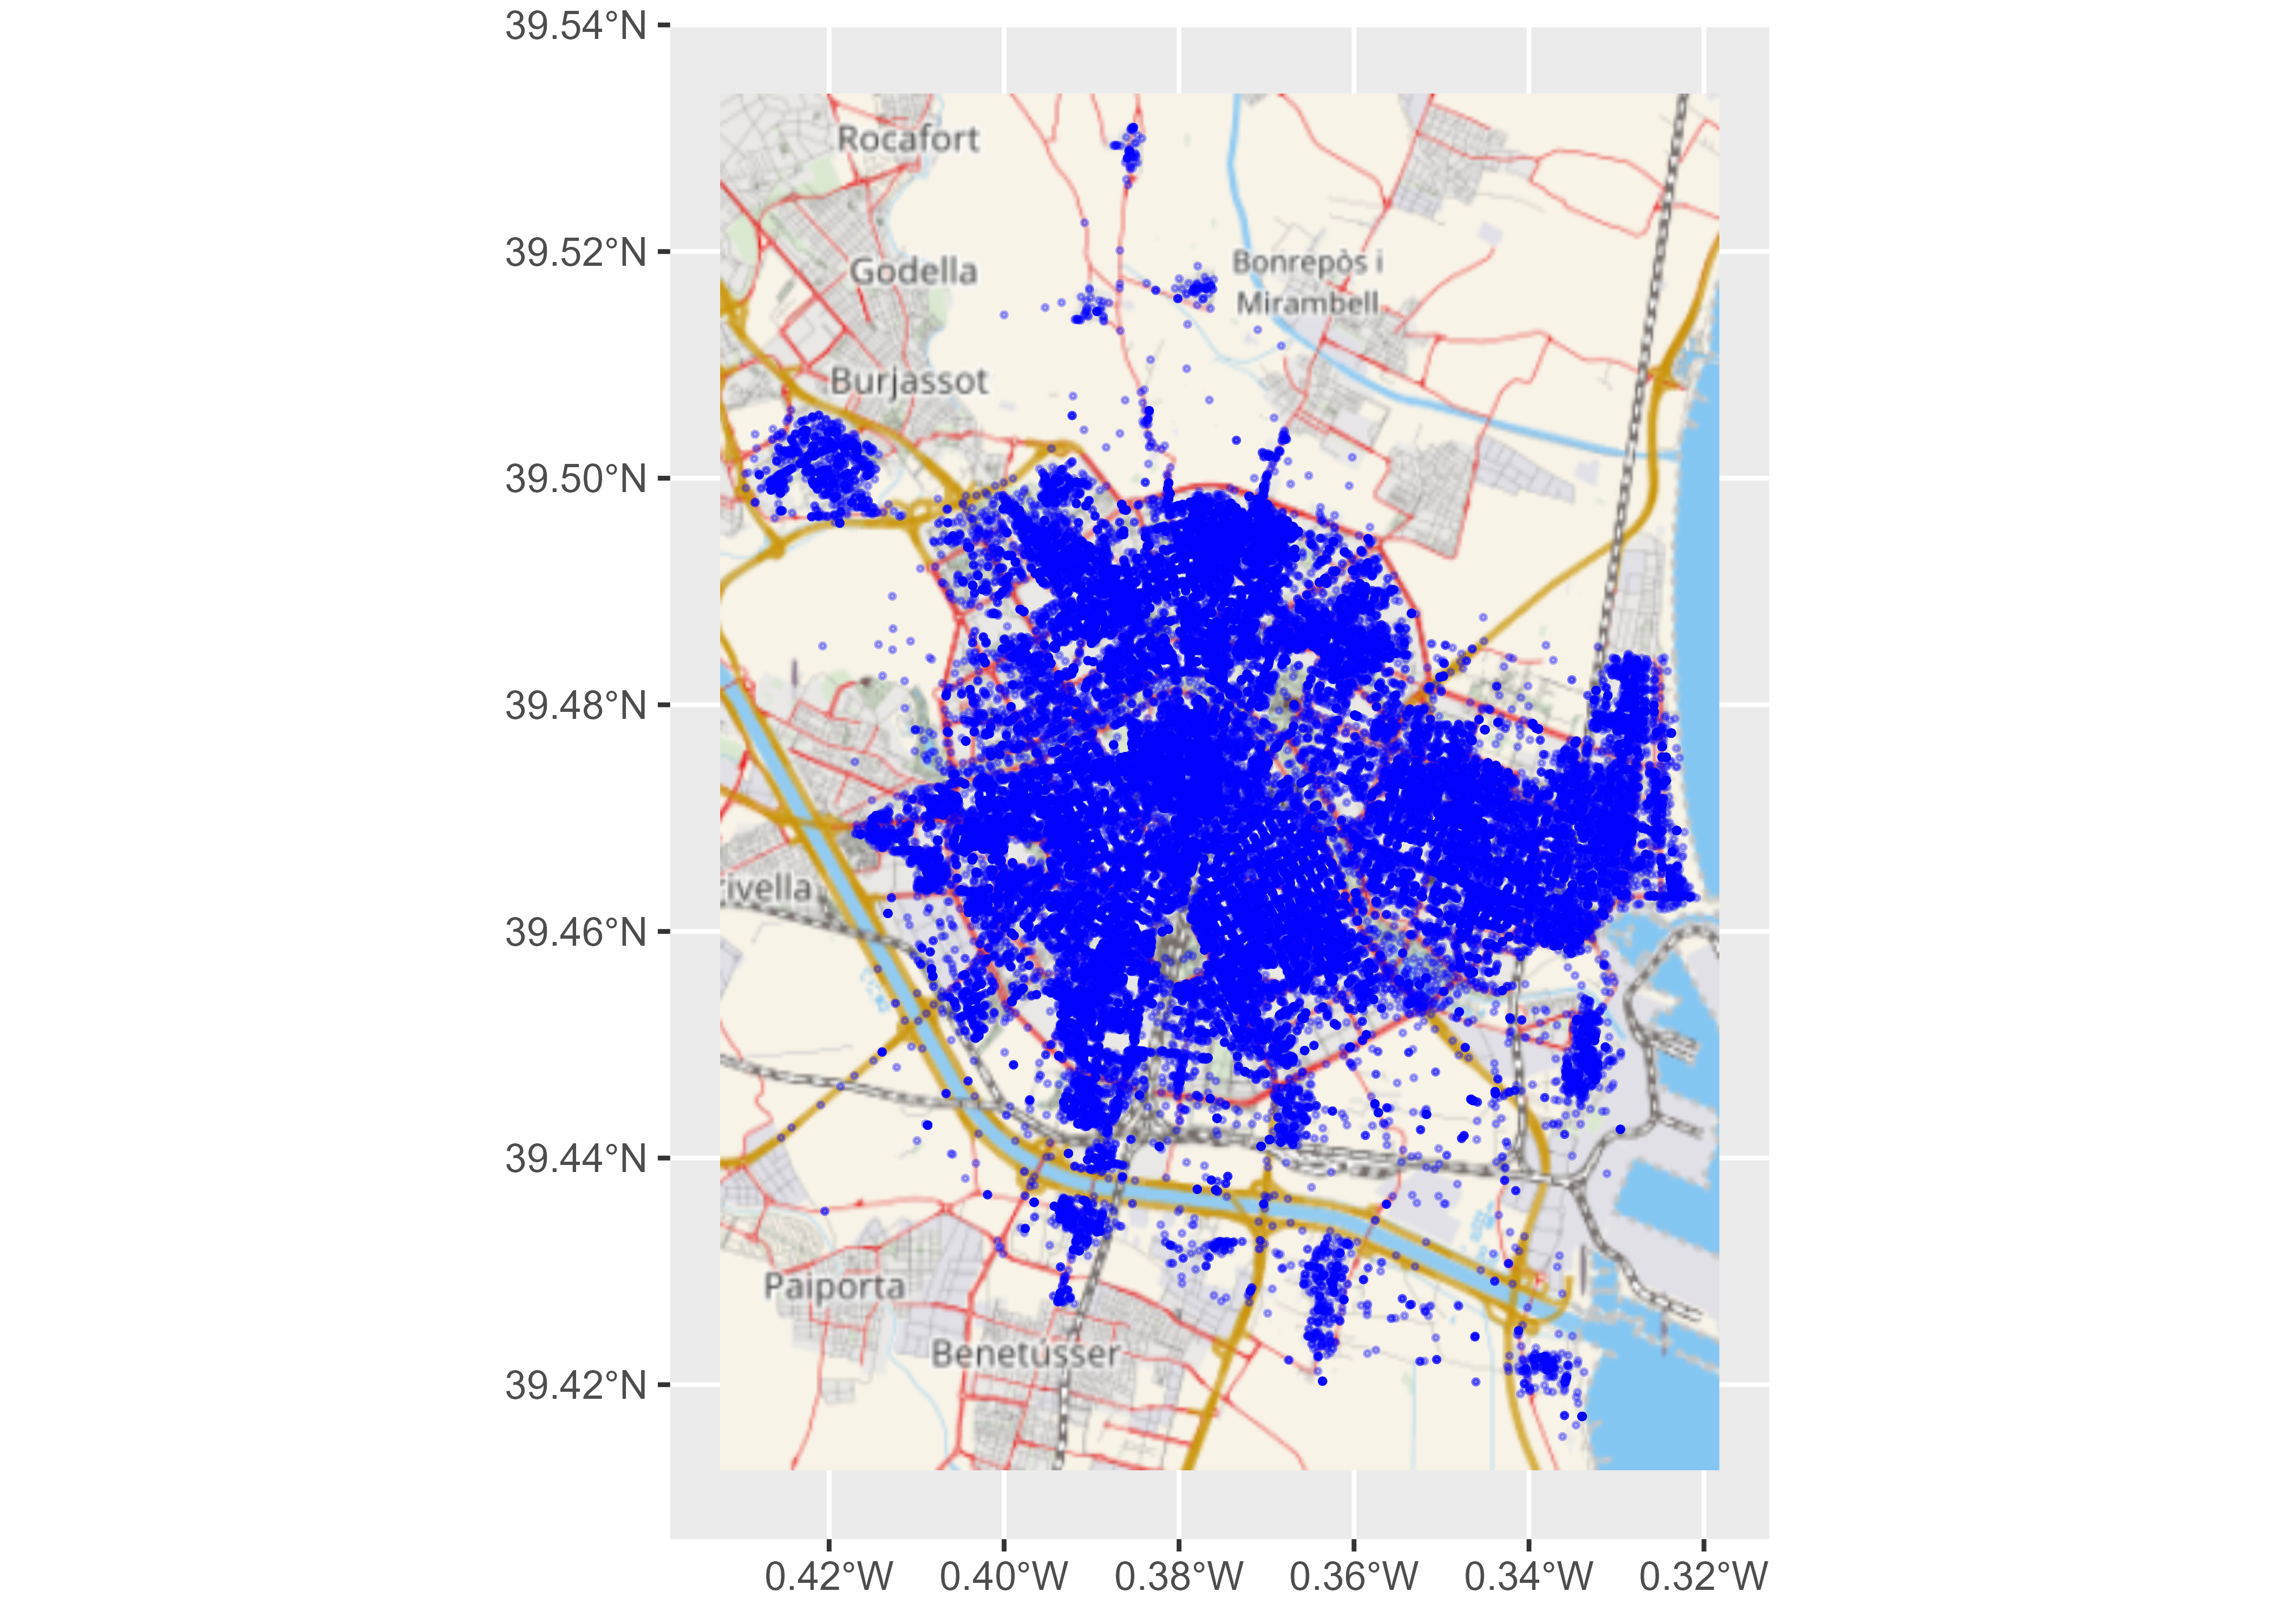
\includegraphics[width=0.6\linewidth]{_main_files/figure-latex/crimen1-1} 

}

\caption{Crímenes en Valencia}\label{fig:crimen1}
\end{figure}

\textbf{Q3: ¿Hay algún patrón en la ocurrencia de crímenes?}

En la Fig. \ref{fig:crimen1} podemos intuir ciertos patrones en la ocurrencia
de crímenes. Por ejemplo, parecen concentrarse en zonas céntricas y no hay
crímenes registrados en la zona del puerto.

Para el siguiente análisis, vamos a analizar el patrón de crímenes del año 2010.

\begin{Shaded}
\begin{Highlighting}[]
\NormalTok{crimen\_2010\_sf }\OtherTok{\textless{}{-}}\NormalTok{ crimen\_sf }\SpecialCharTok{\%\textgreater{}\%}
  \FunctionTok{filter}\NormalTok{(}
\NormalTok{    year }\SpecialCharTok{==} \StringTok{"2010"}
\NormalTok{  )}

\FunctionTok{ggplot}\NormalTok{() }\SpecialCharTok{+}
  \FunctionTok{layer\_spatraster}\NormalTok{(tile) }\SpecialCharTok{+}
  \FunctionTok{geom\_sf}\NormalTok{(}
    \AttributeTok{data =}\NormalTok{ crimen\_2010\_sf,}
    \AttributeTok{col =} \StringTok{"blue"}\NormalTok{,}
    \AttributeTok{size =} \FloatTok{0.3}\NormalTok{,}
    \AttributeTok{alpha =} \FloatTok{0.3}
\NormalTok{  )}
\end{Highlighting}
\end{Shaded}

\begin{figure}

{\centering 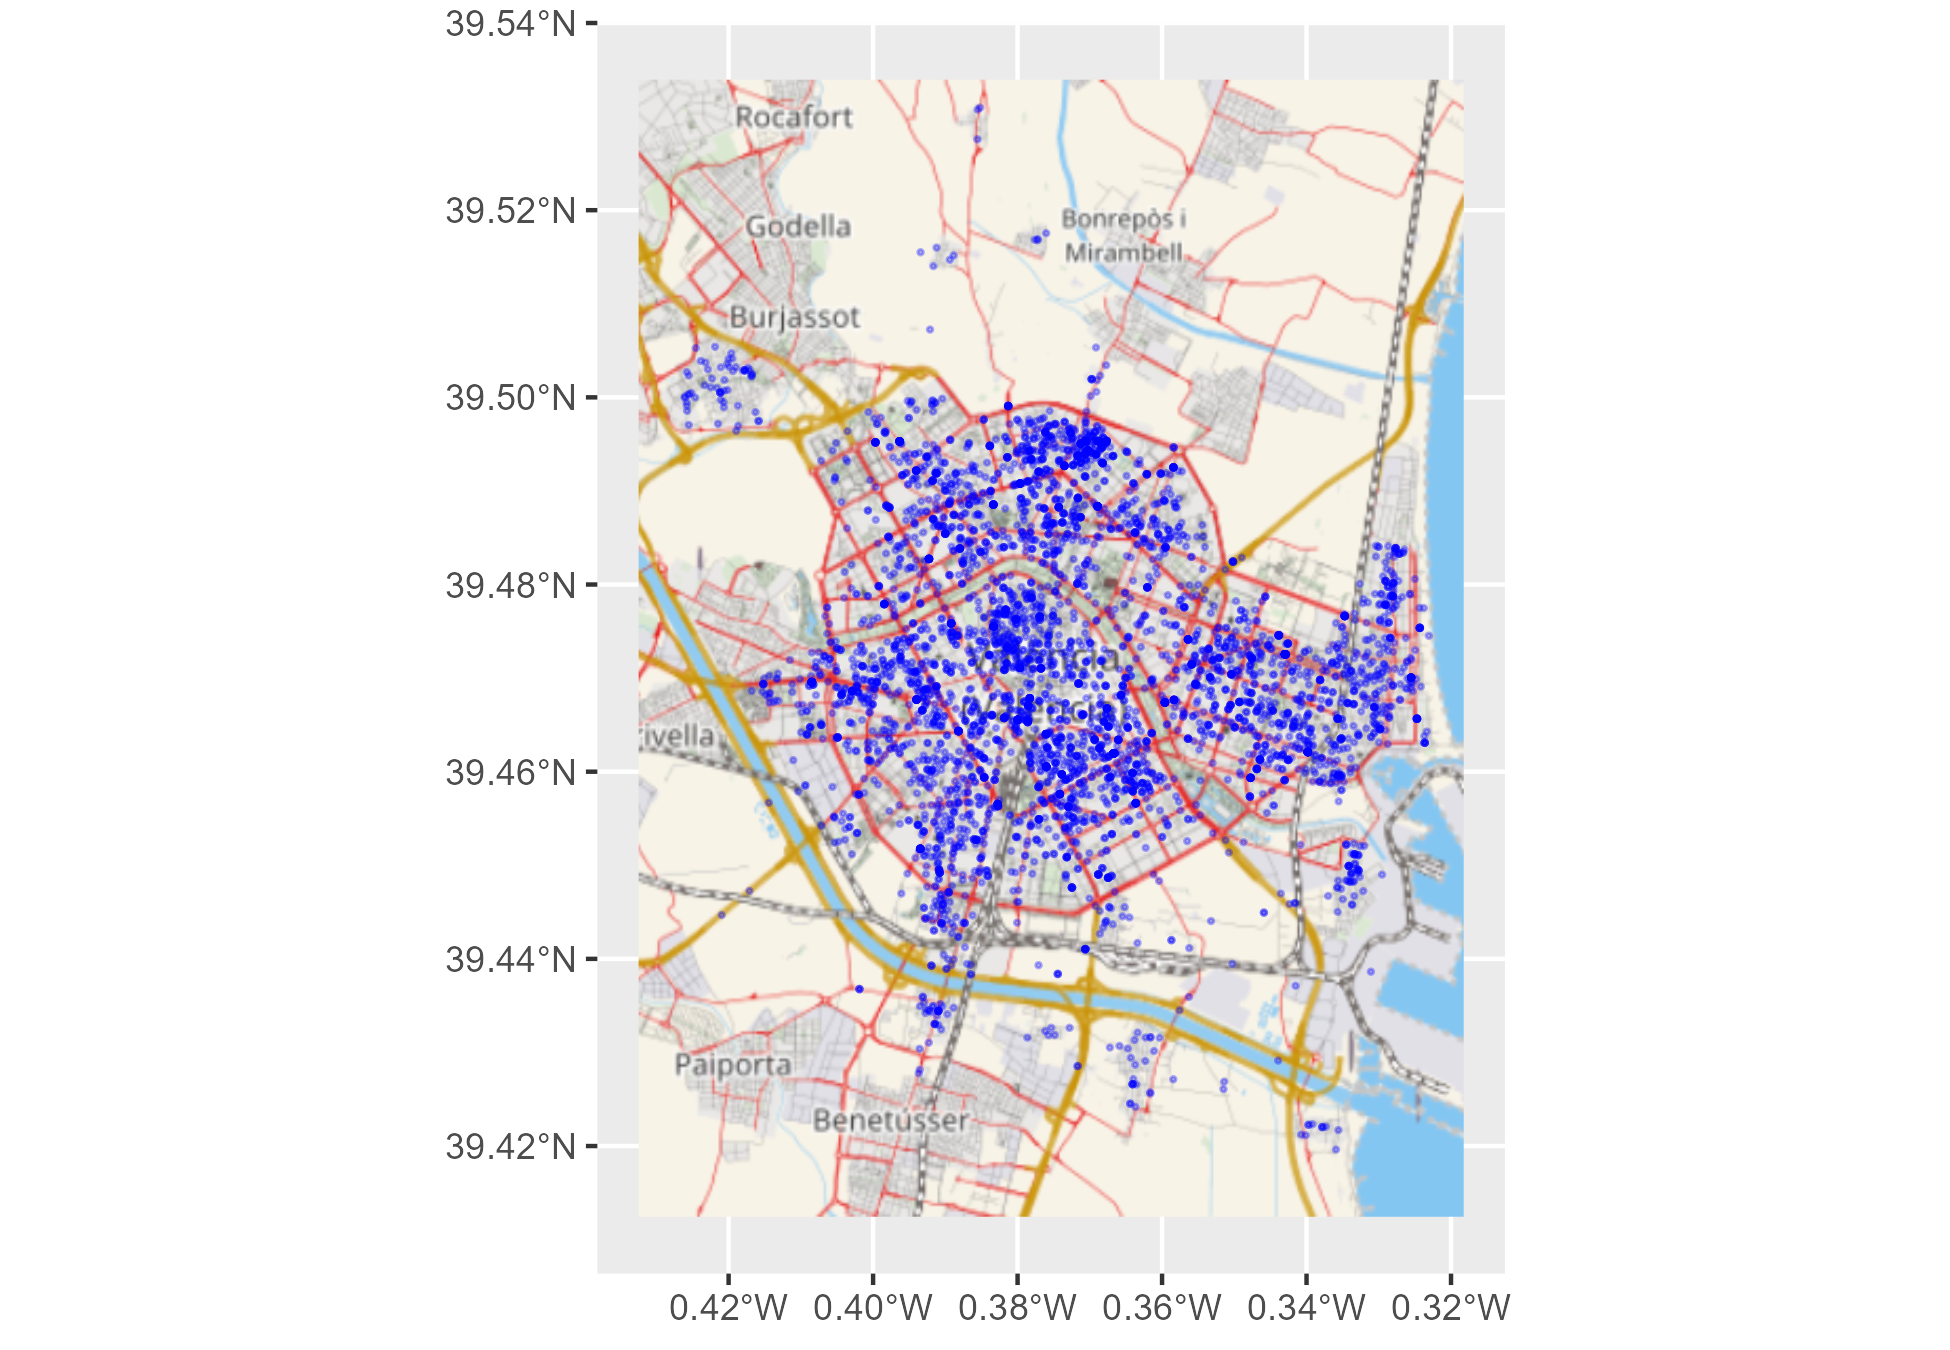
\includegraphics[width=0.6\linewidth]{_main_files/figure-latex/crimen2-1} 

}

\caption{Crímenes en Valencia (2010)}\label{fig:crimen2}
\end{figure}

\emph{Tarea 3: Análisis de patrones con \texttt{spatstat}}

El paquete \texttt{spatstat} (\citet{spatstat_2005}) es el paquete de referencia cuando se
trabaja con patrones de puntos

Siguiendo el anterior ejemplo, vamos a analizar el patrón de crímenes en el año
2010. Además, en el análisis de patrones de puntos es necesario delimitar la
ventana espacial de observación (owin). En este caso será el municipio de
Valencia.

\begin{Shaded}
\begin{Highlighting}[]

\CommentTok{\# Extraigo Valencia con mapSpain}

\NormalTok{valencia }\OtherTok{\textless{}{-}} \FunctionTok{esp\_get\_munic}\NormalTok{(}\AttributeTok{munic =} \StringTok{"\^{}Valencia$"}\NormalTok{) }\SpecialCharTok{\%\textgreater{}\%}
  \CommentTok{\# Necesito proyectar, en este caso usamos ETRS89{-}UTM huso 30 EPSG:25830}
  \FunctionTok{st\_transform}\NormalTok{(}\DecValTok{25830}\NormalTok{)}



\FunctionTok{library}\NormalTok{(spatstat)}
\CommentTok{\# Necesitamos un recinto de observación: owin}

\NormalTok{val\_owin }\OtherTok{\textless{}{-}} \FunctionTok{as.owin}\NormalTok{(valencia)}

\CommentTok{\# Extraemos las coordenadas de los crímenes. Han de estar en el mismo CRS}
\CommentTok{\# que el owin}

\NormalTok{coords }\OtherTok{\textless{}{-}}\NormalTok{ crimen\_2010\_sf }\SpecialCharTok{\%\textgreater{}\%}
  \FunctionTok{st\_transform}\NormalTok{(}\DecValTok{25830}\NormalTok{) }\SpecialCharTok{\%\textgreater{}\%}
  \FunctionTok{st\_coordinates}\NormalTok{()}

\NormalTok{mydata\_ppp }\OtherTok{\textless{}{-}} \FunctionTok{ppp}\NormalTok{(}
  \AttributeTok{x =} \FunctionTok{as.numeric}\NormalTok{(coords[, }\DecValTok{1}\NormalTok{]),}
  \AttributeTok{y =} \FunctionTok{as.numeric}\NormalTok{(coords[, }\DecValTok{2}\NormalTok{]),}
  \AttributeTok{window =}\NormalTok{ val\_owin}
\NormalTok{)}

\FunctionTok{plot}\NormalTok{(mydata\_ppp)}
\end{Highlighting}
\end{Shaded}

\begin{center}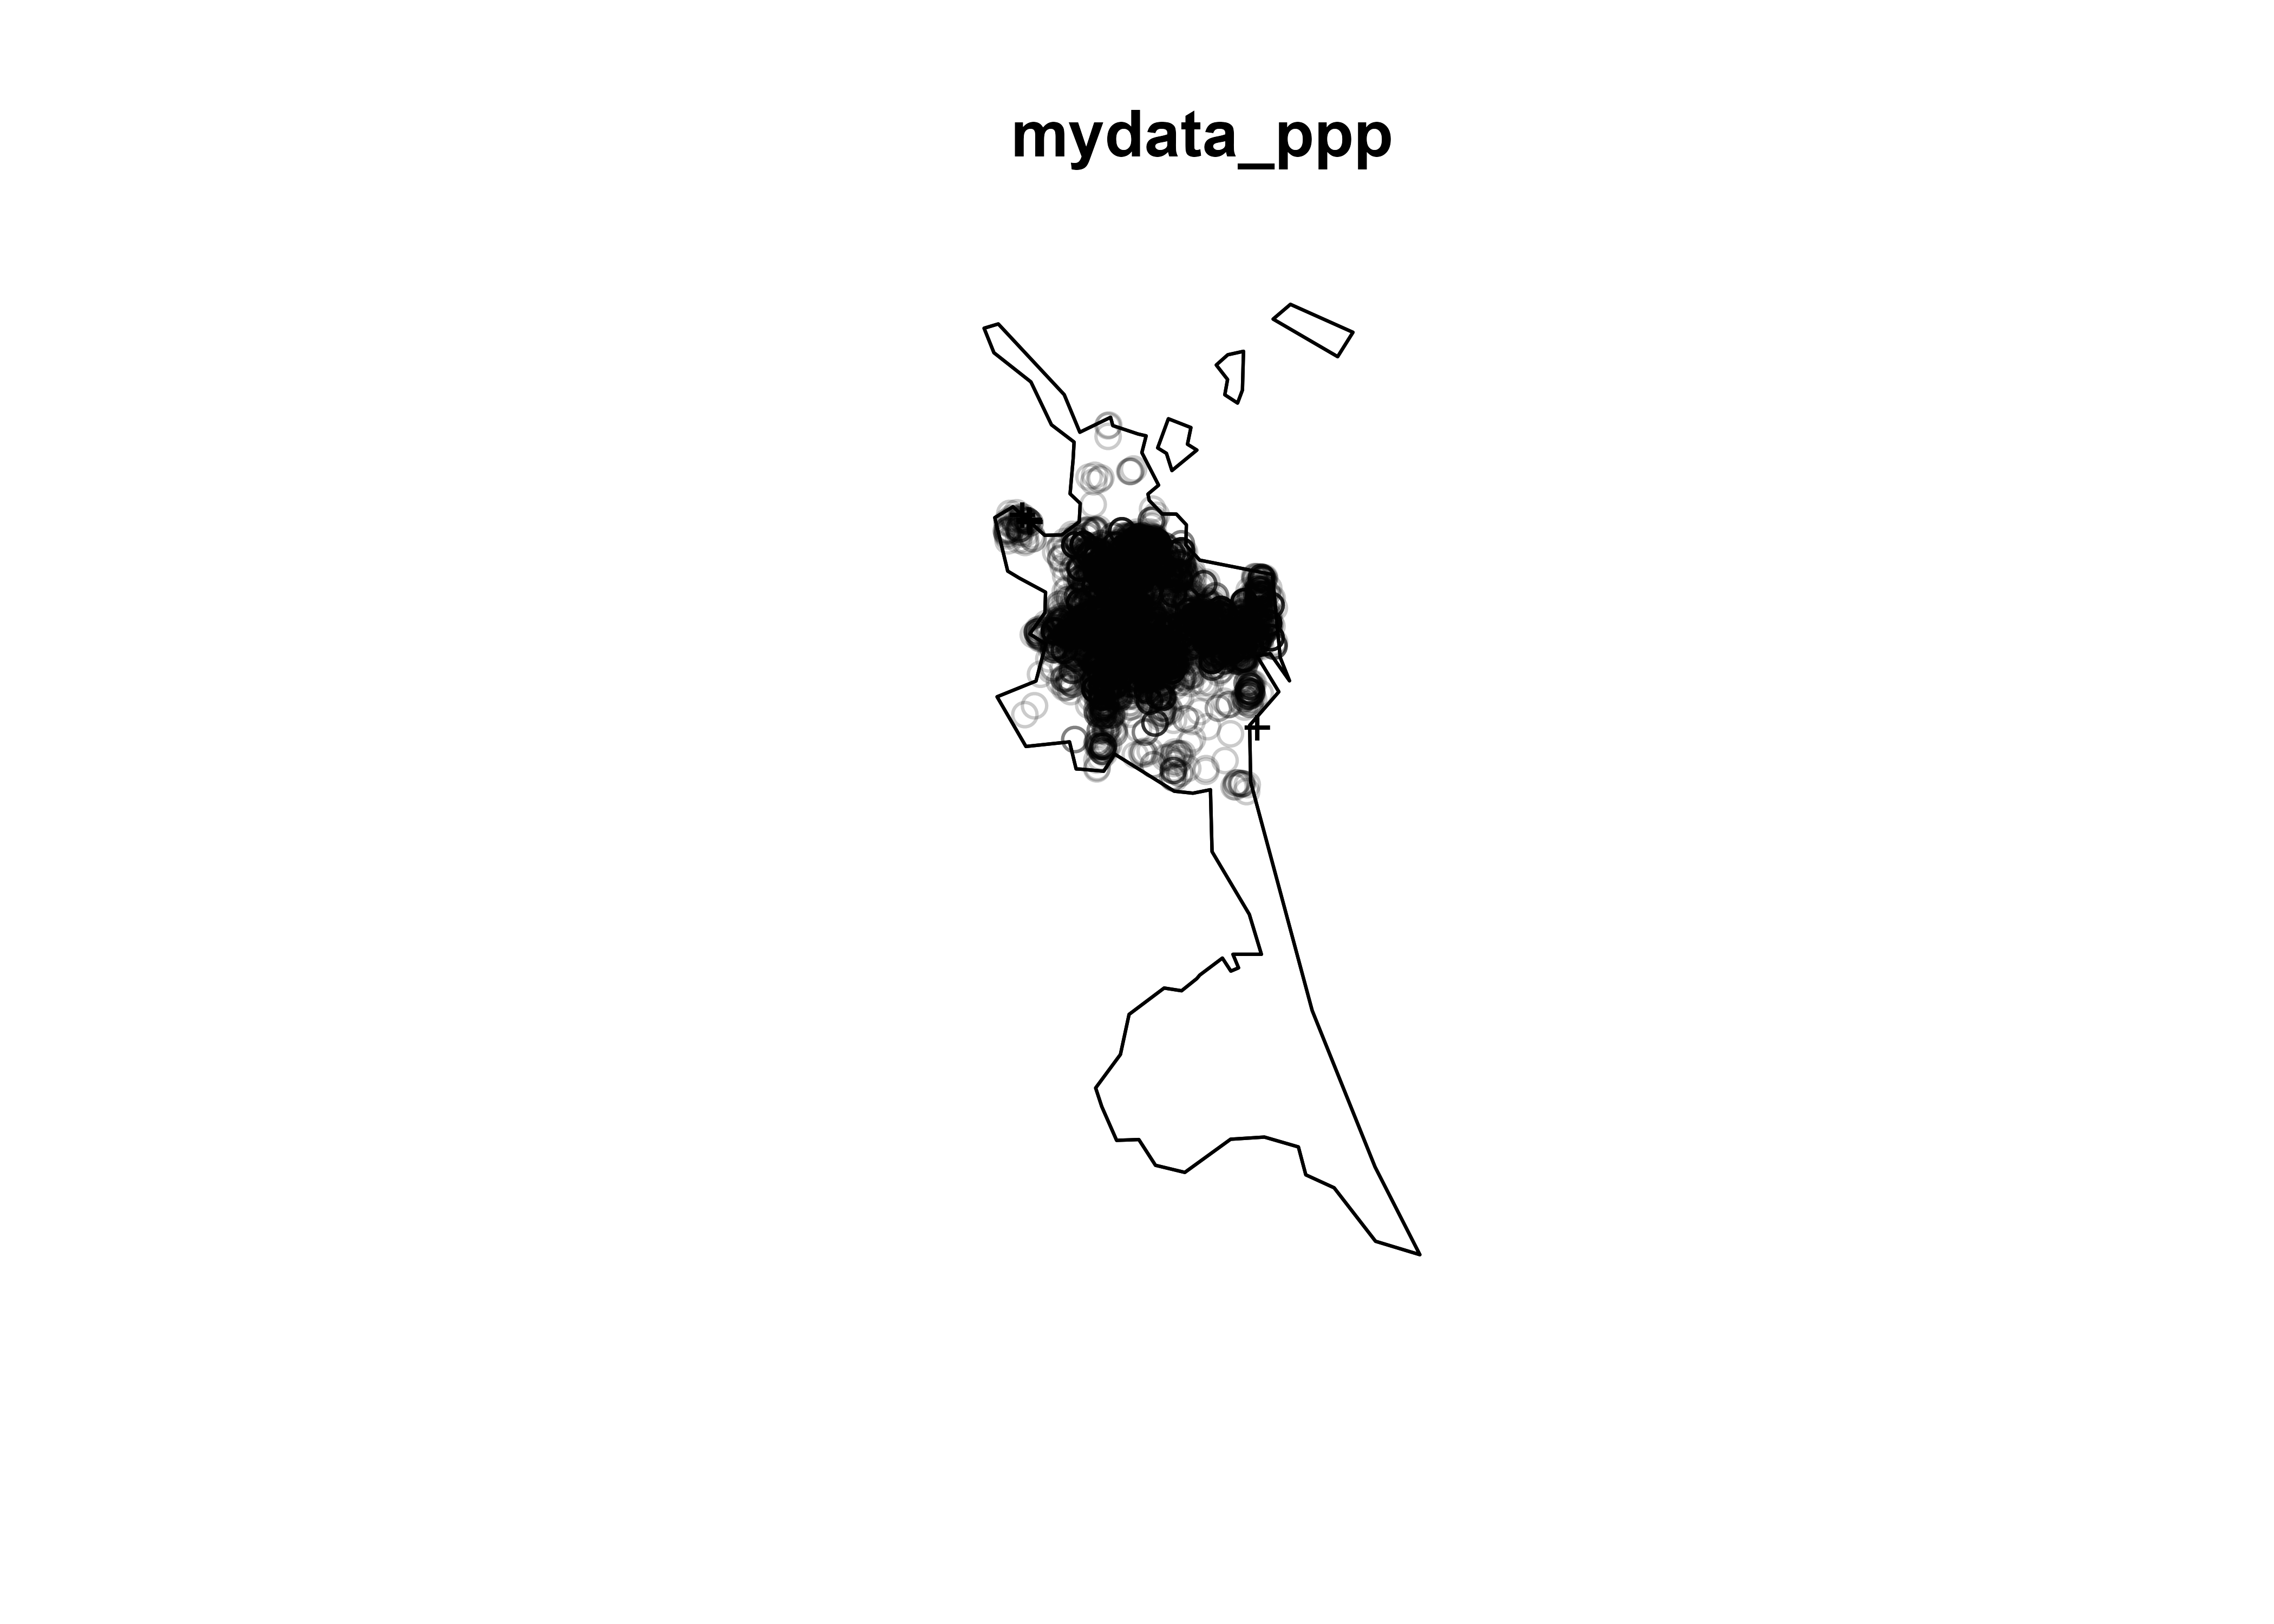
\includegraphics[width=0.6\linewidth]{_main_files/figure-latex/objeto_ppp-1} \end{center}

\textbf{Q4: ¿Qué información contiene nuestro objeto en formato ppp?}

\begin{Shaded}
\begin{Highlighting}[]
\FunctionTok{summary}\NormalTok{(mydata\_ppp)}
\CommentTok{\#\textgreater{} Planar point pattern:  5332 points}
\CommentTok{\#\textgreater{} Average intensity 3.917619e{-}05 points per square unit}
\CommentTok{\#\textgreater{} }
\CommentTok{\#\textgreater{} *Pattern contains duplicated points*}
\CommentTok{\#\textgreater{} }
\CommentTok{\#\textgreater{} Coordinates are given to 1 decimal place}
\CommentTok{\#\textgreater{} i.e. rounded to the nearest multiple of 0.1 units}
\CommentTok{\#\textgreater{} }
\CommentTok{\#\textgreater{} Window: polygonal boundary}
\CommentTok{\#\textgreater{} 4 separate polygons (no holes)}
\CommentTok{\#\textgreater{}            vertices      area relative.area}
\CommentTok{\#\textgreater{} polygon 1         4   1977930       0.01450}
\CommentTok{\#\textgreater{} polygon 2        82 131953000       0.97000}
\CommentTok{\#\textgreater{} polygon 3         7    958085       0.00704}
\CommentTok{\#\textgreater{} polygon 4         7   1214060       0.00892}
\CommentTok{\#\textgreater{} enclosing rectangle: [720573.4, 735116.6] x [4351274, 4382995] units}
\CommentTok{\#\textgreater{}                      (14540 x 31720 units)}
\CommentTok{\#\textgreater{} Window area = 136103000 square units}
\CommentTok{\#\textgreater{} Fraction of frame area: 0.295}
\CommentTok{\#\textgreater{} }
\CommentTok{\#\textgreater{} *** 6 illegal points stored in attr(,"rejects") ***}
\end{Highlighting}
\end{Shaded}

\emph{Tarea 4: Cálculo de la densidad mediante cuadrantes.}

Es importante determinar si los puntos se distribuyen al azar o tienen algún
patrón. Por ello, lo primero que haremos será representar el objeto \texttt{feb\_ppp} y
superponer unos cuadrantes para su comportamiento (véase Fig.
\ref{fig:cuadrante}).

\begin{Shaded}
\begin{Highlighting}[]
\DocumentationTok{\#\# Hallamos los cuadrantes}
\NormalTok{cuadrante }\OtherTok{\textless{}{-}} \FunctionTok{quadratcount}\NormalTok{(mydata\_ppp,}
  \AttributeTok{nx =} \DecValTok{5}\NormalTok{,}
  \AttributeTok{ny =} \DecValTok{5}
\NormalTok{)}

\DocumentationTok{\#\# Dibujamos el número de crímenes que hay en cada cuadrante}
\FunctionTok{plot}\NormalTok{(mydata\_ppp, }\AttributeTok{pch =} \DecValTok{1}\NormalTok{, }\AttributeTok{main =} \StringTok{""}\NormalTok{)}
\FunctionTok{plot}\NormalTok{(cuadrante, }\AttributeTok{add =} \ConstantTok{TRUE}\NormalTok{, }\AttributeTok{col =} \StringTok{"red"}\NormalTok{, }\AttributeTok{cex =} \FloatTok{1.2}\NormalTok{)}
\end{Highlighting}
\end{Shaded}

\begin{figure}

{\centering 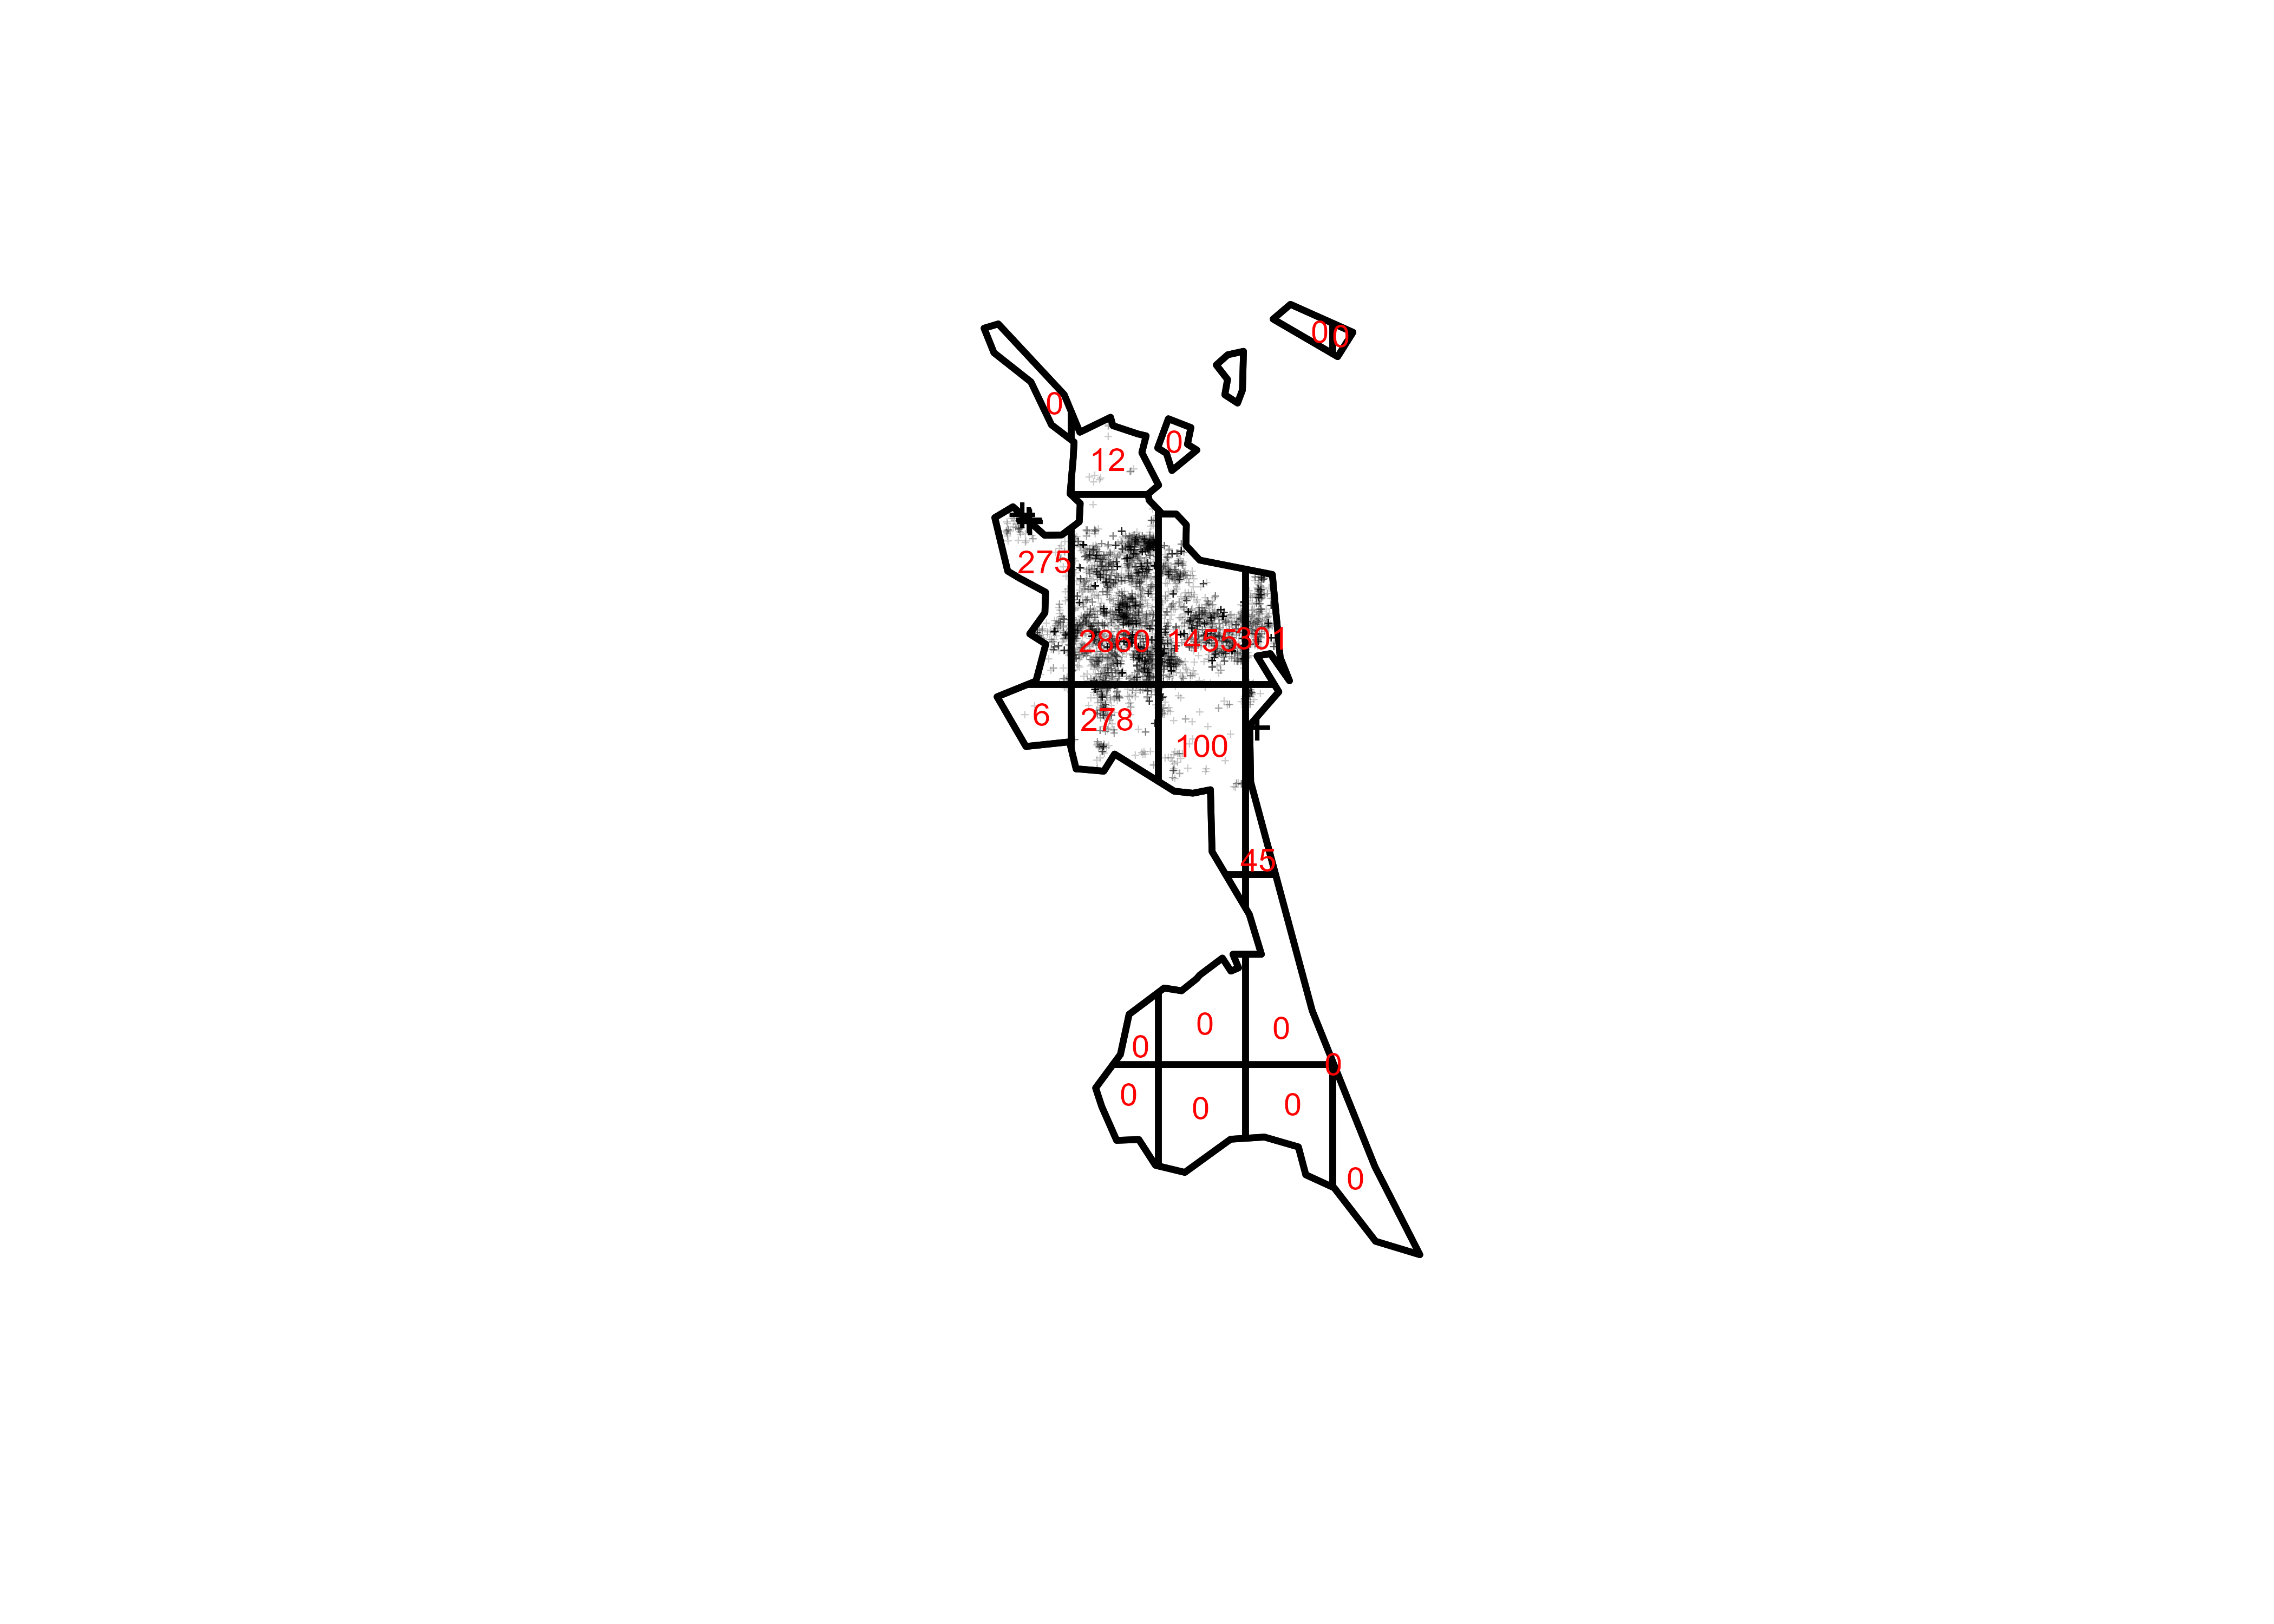
\includegraphics[width=0.6\linewidth]{_main_files/figure-latex/cuadrante-1} 

}

\caption{Crímenes en Valencia por cuadrantes (2010)}\label{fig:cuadrante}
\end{figure}

Como se puede apreciar en la Fig. \ref{fig:cuadrante} hay cuadrantes que
registran cero crímenes y otros que registran hasta 2.860 crímenes.

\emph{Tarea 5: Estimación de la densidad de patrones de puntos.}

En la Fig. \ref{fig:intensidad-ripley} se muestra la gráfica de la estimación
usando la K de Ripley. Los conocimientos teóricos necesarios para llevar a cabo
este tipo de estimación se verán en el tema \textbf{Patrones de Puntos}. El objetivo
de este ejemplo es meramente ilustrativo.

\begin{Shaded}
\begin{Highlighting}[]
\NormalTok{densidad }\OtherTok{\textless{}{-}} \FunctionTok{density}\NormalTok{(mydata\_ppp)}
\FunctionTok{plot}\NormalTok{(densidad, }\AttributeTok{main =} \StringTok{" "}\NormalTok{)}
\FunctionTok{points}\NormalTok{(mydata\_ppp, }\AttributeTok{pch =} \StringTok{"+"}\NormalTok{, }\AttributeTok{cex =} \FloatTok{0.5}\NormalTok{)}
\end{Highlighting}
\end{Shaded}

\begin{figure}

{\centering 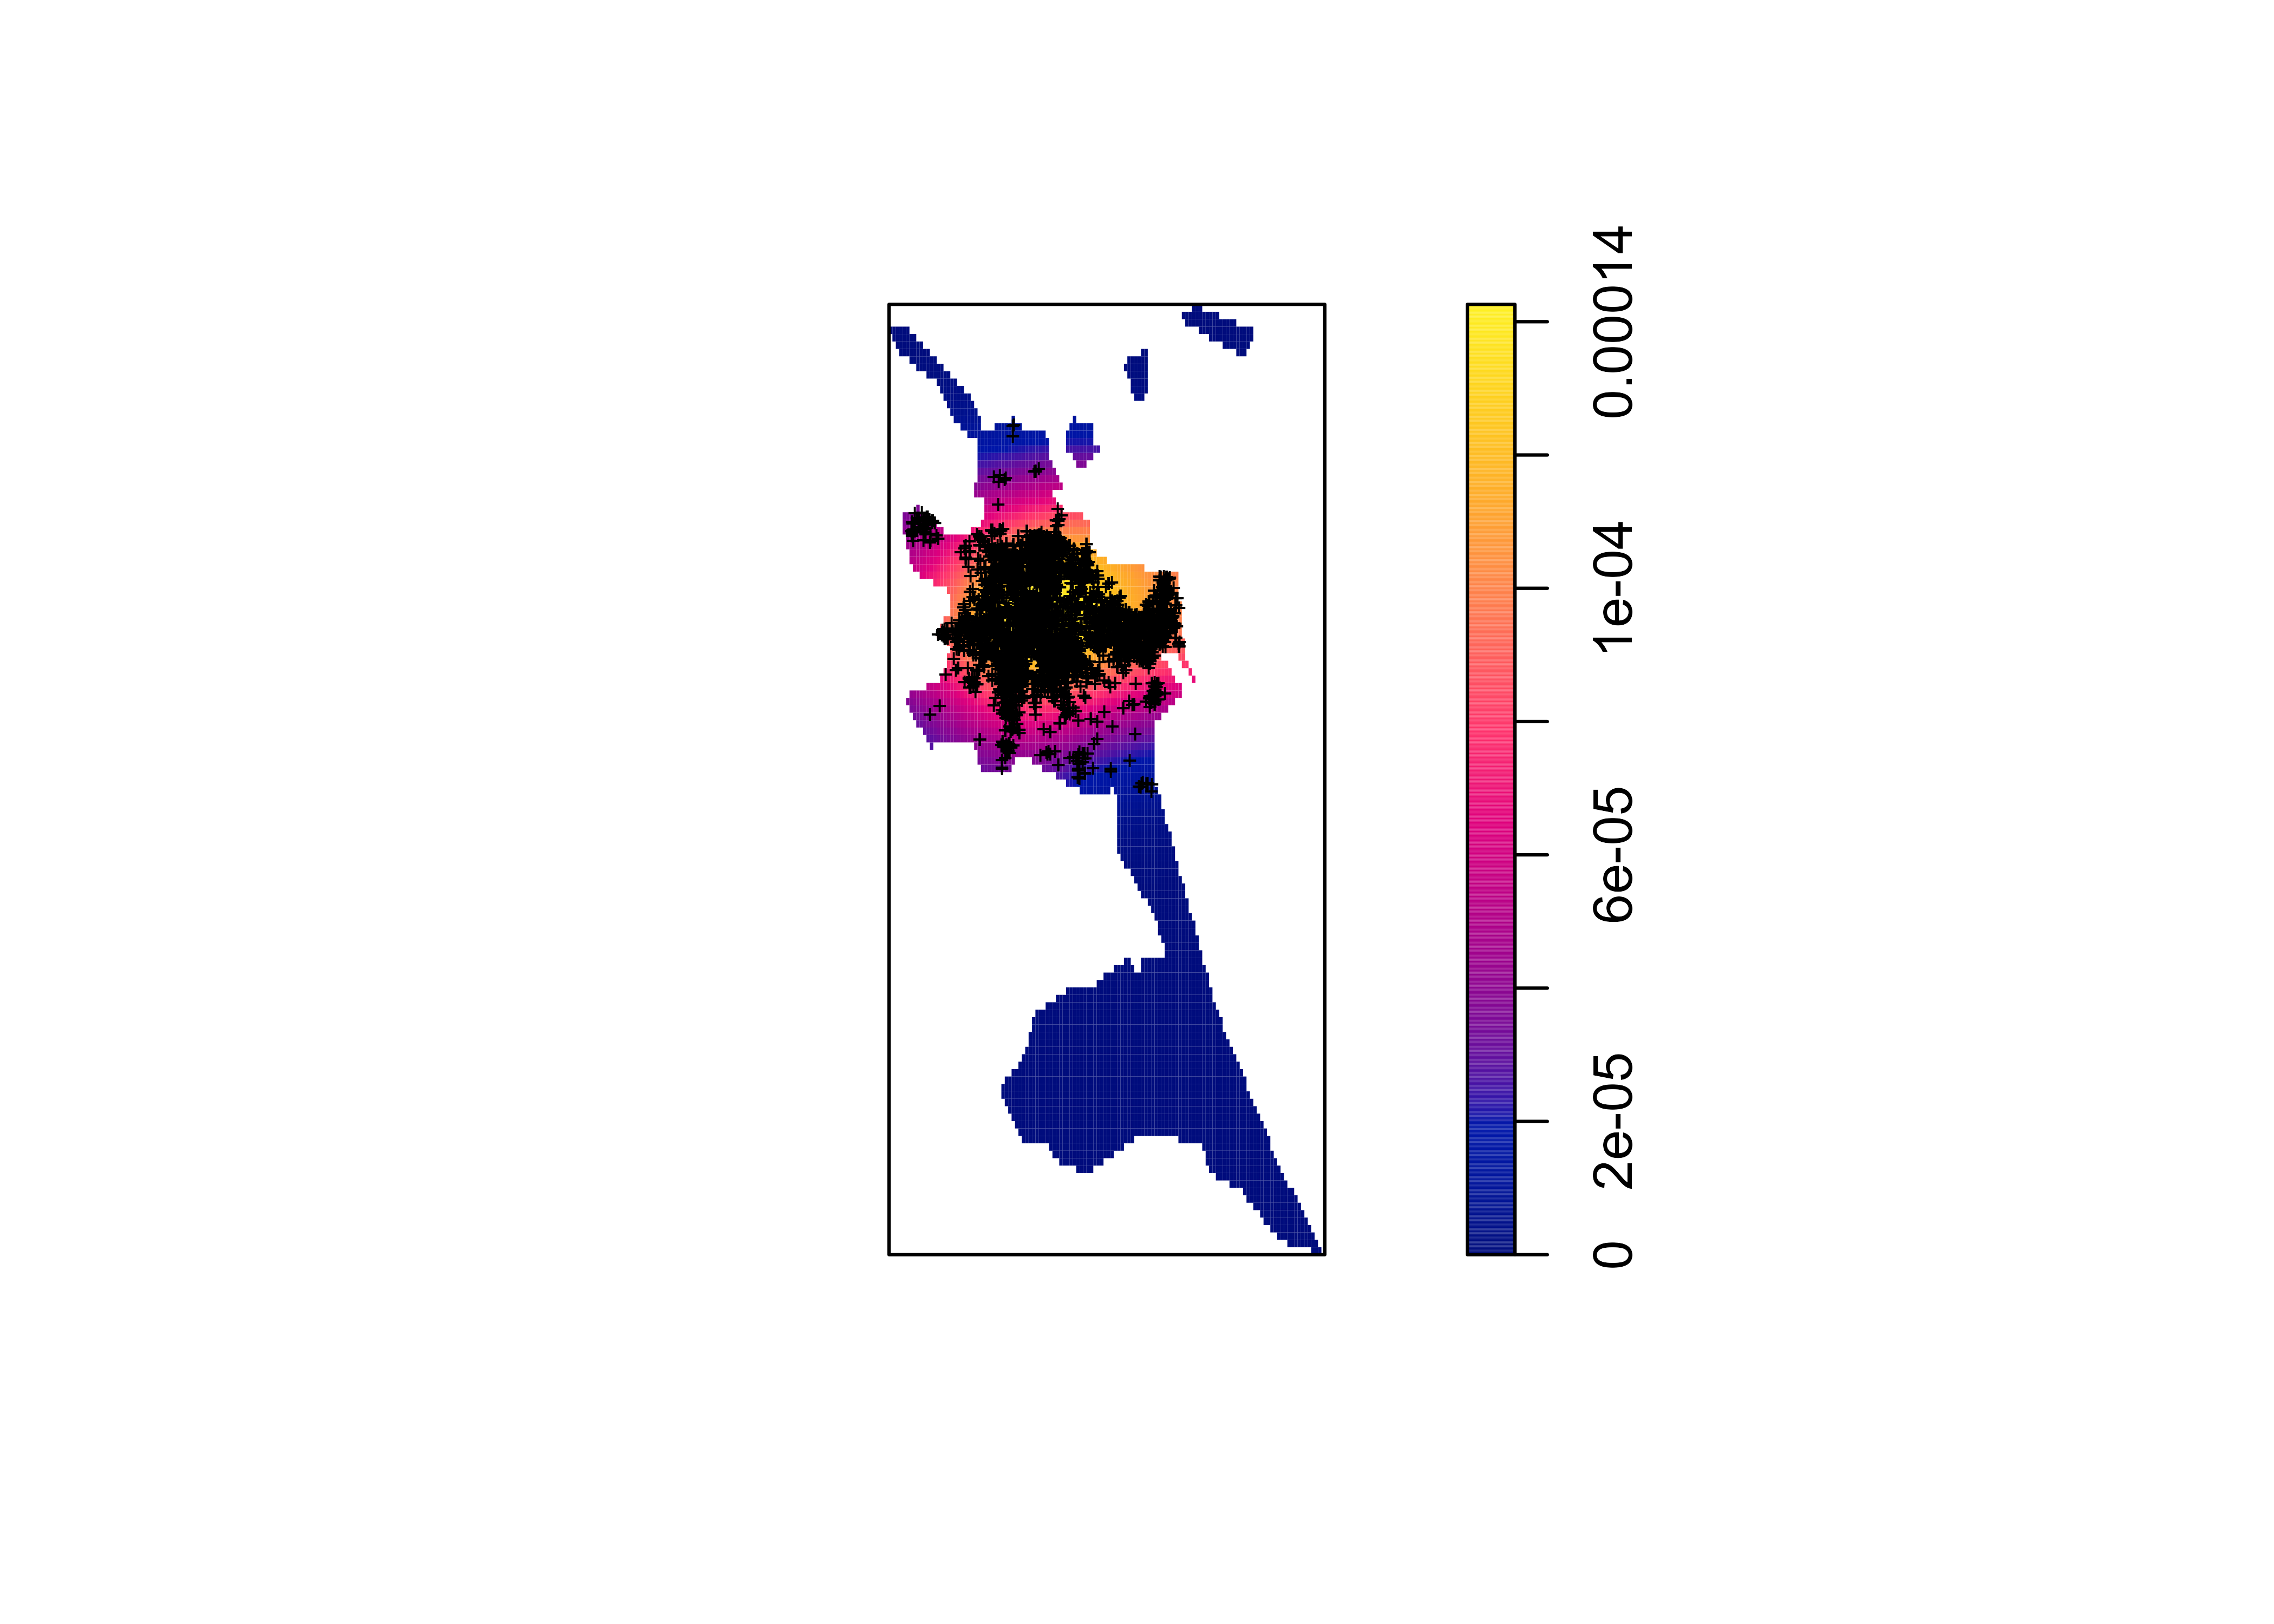
\includegraphics[width=0.6\linewidth]{_main_files/figure-latex/intensidad-ripley-1} 

}

\caption{Intensidad de crímenes estimada con la K-Ripley}\label{fig:intensidad-ripley}
\end{figure}

\hypertarget{referencias}{%
\chapter{Referencias}\label{referencias}}

\hypertarget{appendix-anexo}{%
\appendix}


\hypertarget{crsproy}{%
\chapter{Tipos de CRS proyectados}\label{crsproy}}

Existen varias familias de proyecciones, que se pueden clasificar de diversas
maneras: por tipo de superficie de proyección y por métrica a preservar.

\hypertarget{por-tipo-de-superficie-de-proyecciuxf3n}{%
\section{Por tipo de superficie de proyección}\label{por-tipo-de-superficie-de-proyecciuxf3n}}

El proceso de trasladar puntos de una esfera a un plano puede plantearse de
manera práctica como el ejercicio de envolver una esfera con una superificie
plana (como una hoja de papel) y trasladar los puntos de la esfera de manera
lineal al punto de la superficie plana más cercano a ella. La Fig.
\ref{fig:fi-proys} muestra estos tres tipos de proyección.

\begin{figure}

{\centering 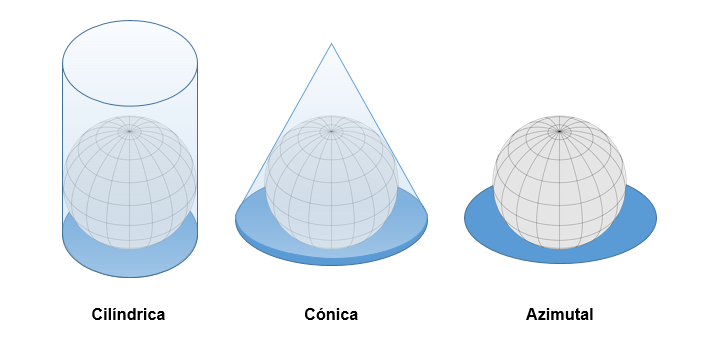
\includegraphics[width=0.6\linewidth]{img/tipos_proy} 

}

\caption{Tipos de proyección por superficie de proyección}\label{fig:fi-proys}
\end{figure}

A partir de este ejercicio, se plantean tres posibles soluciones (cilíndrica,
cónica y acimutal o planar), dependiendo del tipo de superficie que se use para
proyectar.

\begin{itemize}
\tightlist
\item
  \textbf{Proyecciones cilíndricas}: Son aquellas proyecciones donde la superficie
  de proyección conforma un cilindro alrededor de la Tierra. Una de las
  proyecciones cilíndricas más conocidas es la \textbf{proyección de Mercator} (Ver
  Fig. \ref{fig:mercator}).
\end{itemize}

\begin{figure}

{\centering 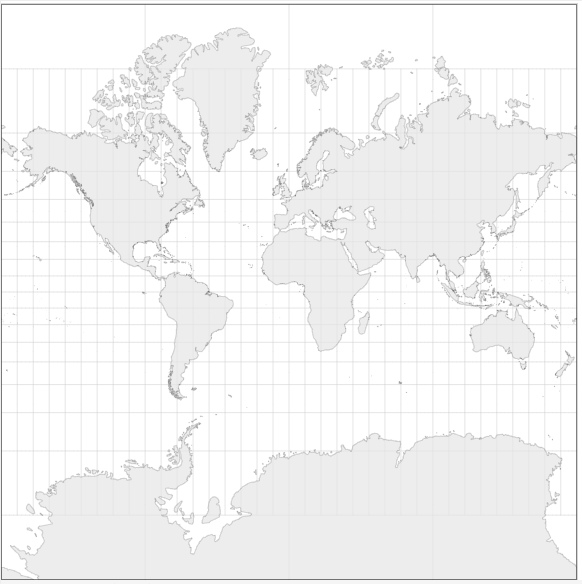
\includegraphics[width=0.4\linewidth]{img/mercator} 

}

\caption{Proyección Mercator}\label{fig:mercator}
\end{figure}

\begin{itemize}
\tightlist
\item
  \textbf{Proyecciones cónicas}: En este tipo de proyecciones, se plantea la
  superficie de proyección como una forma cónica. Como ejemplo, la
  \textbf{proyección cónica equiáreas de Albers} es una de las proyecciones que más
  suele usarse en la representación de mapas de América del Norte (Ver Fig.
  \ref{fig:albers}).
\end{itemize}

\begin{figure}

{\centering 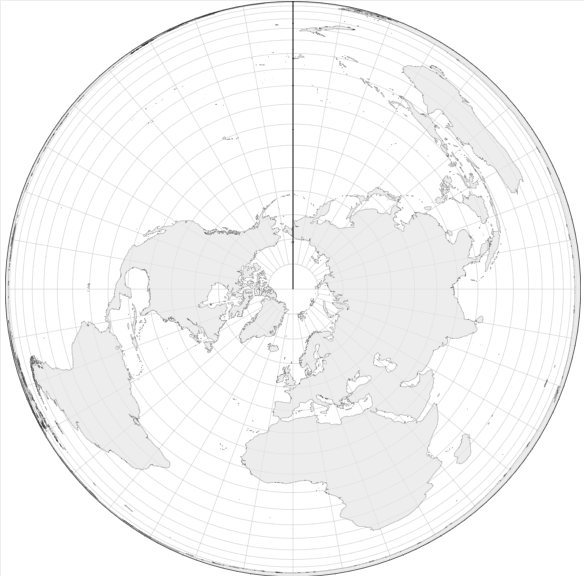
\includegraphics[width=0.4\linewidth]{img/albers_conic} 

}

\caption{Proyección cónica equiáreas de Albers}\label{fig:albers}
\end{figure}

\begin{itemize}
\tightlist
\item
  \textbf{Proyecciones acimutales o planares:} En este tipo de proyección se
  proyecta una porción de la Tierra sobre un plano que es tangente a la misma
  en el punto de referencia. Como ejemplos de proyecciones acimutales podemos
  destacar la \textbf{proyección ortográfica} (Ver Fig. \ref{fig:orto}).
\end{itemize}

\begin{figure}

{\centering 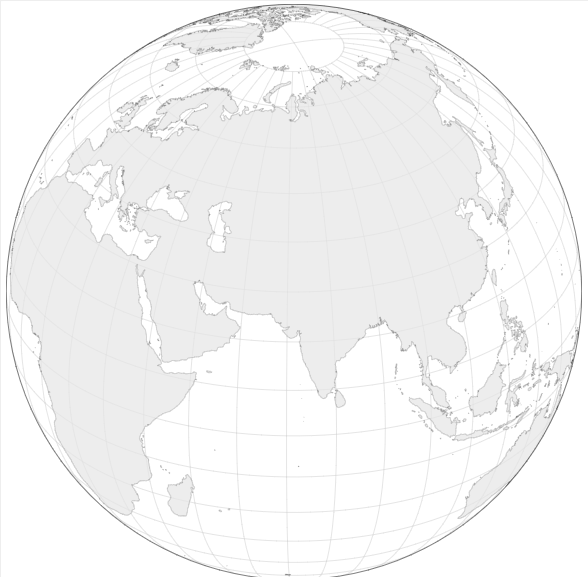
\includegraphics[width=0.4\linewidth]{img/orto} 

}

\caption{Proyección ortogonal}\label{fig:orto}
\end{figure}

\hypertarget{por-muxe9trica-a-preservar}{%
\section{Por métrica a preservar}\label{por-muxe9trica-a-preservar}}

Es importante tener en cuenta que cualquier proyección de la superficie de la
Tierra produce distorsiones en una o varias características geográficas. Como
ejemplo clásico, la proyección de Mercator produce distorsiones del \textbf{tamaño}
especialmente en aquellas regiones más cercanas a los polos (Groenlandia, que la
proyección de Mercator presenta una área similar a la de África, tiene menor
superficie real que Argelia). Otras de las métricas que suele verse
distorsionada son la \textbf{distancia} entre dos puntos geográficos, la
\textbf{dirección} o la \textbf{forma} de regiones de la Tierra.

A lo largo de la Historia se han desarrollado diversas proyecciones cuyo
objetivo es preservar alguna o varias de las propiedades mencionadas
anteriormente, sin embargo es importante destacar que \textbf{no existe una proyección
que sea capaz de preservar todas las métricas a la vez}.

Según la metrica a presevar, las proyecciones se pueden clasificar en:

\begin{itemize}
\tightlist
\item
  \textbf{Proyecciones conformales:} Intentan preservar los \textbf{ángulos} que se
  forman en la superficie terrestre. Por ejemplo, la proyección de Mercator
  representa ángulos rectos en las intersecciones de los paralelos y los
  meridianos (Ver Fig. \ref{fig:conform}).
\end{itemize}

\begin{figure}

{\centering 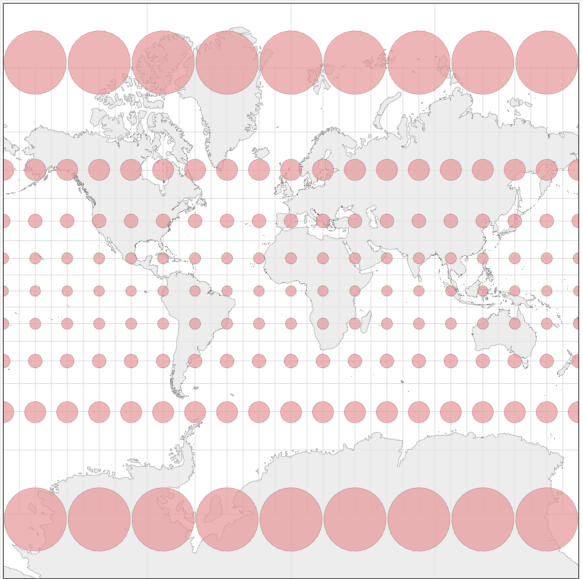
\includegraphics[width=0.3\linewidth]{img/conform} 

}

\caption{Ejemplo de proyección conformal: Mercator}\label{fig:conform}
\end{figure}

\begin{itemize}
\tightlist
\item
  \textbf{Proyecciones equivalentes}: Preservan las proporciones de las \textbf{áreas},
  provocando a su vez deformaciones en el resto de características, como la
  forma o los ángulos. La proyección acimutal equivalente de Lambers es un
  tipo de proyección equivalente (Ver Fig. \ref{fig:equiv}).
\end{itemize}

\begin{figure}

{\centering 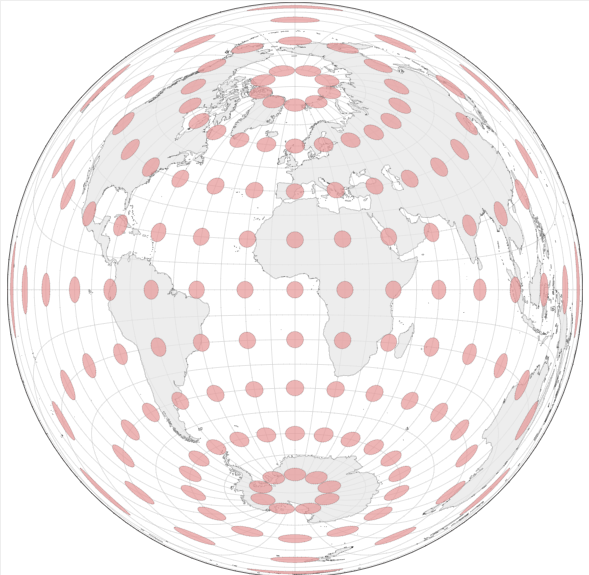
\includegraphics[width=0.3\linewidth]{img/equiv} 

}

\caption{Ejemplo de proyección equivalente: Proyección acimutal equivalente de Lambers}\label{fig:equiv}
\end{figure}

\begin{itemize}
\tightlist
\item
  \textbf{Proyecciones equidistantes:} Preservan la \textbf{distancia} entre dos puntos
  geográficos específicos. Por ejemplo, la proyección Plate carré preserva la
  distancia entre el Polo Norte y el Polo Sur (Ver Fig. \ref{fig:equidist}).
\end{itemize}

\begin{figure}

{\centering 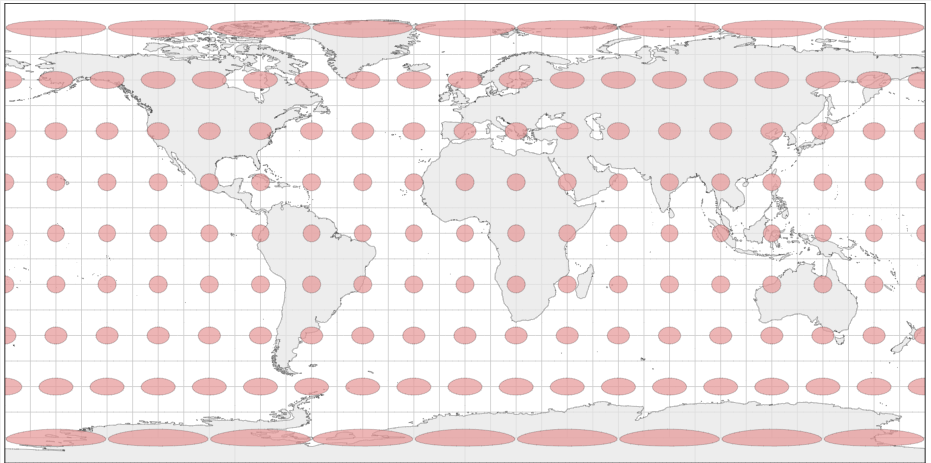
\includegraphics[width=0.3\linewidth]{img/equidist} 

}

\caption{Ejemplo de proyección equidistante: Platé carre}\label{fig:equidist}
\end{figure}

\begin{itemize}
\tightlist
\item
  \textbf{Proyecciones de compromiso}: No intentan preservar ninguna métrica en
  concreto. En su lugar, se centran en intentar encontrar un \textbf{equilibrio}
  entre las diversas distorsiones que provocan para intentar dar una
  representación más o menos representativa de la superficie terrestre. La
  proyección de Winkel Tripel, usada en los mapas de National Geographic, es
  un ejemplo de proyección de compromiso (Ver Fig. \ref{fig:comp}).
\end{itemize}

\begin{figure}

{\centering 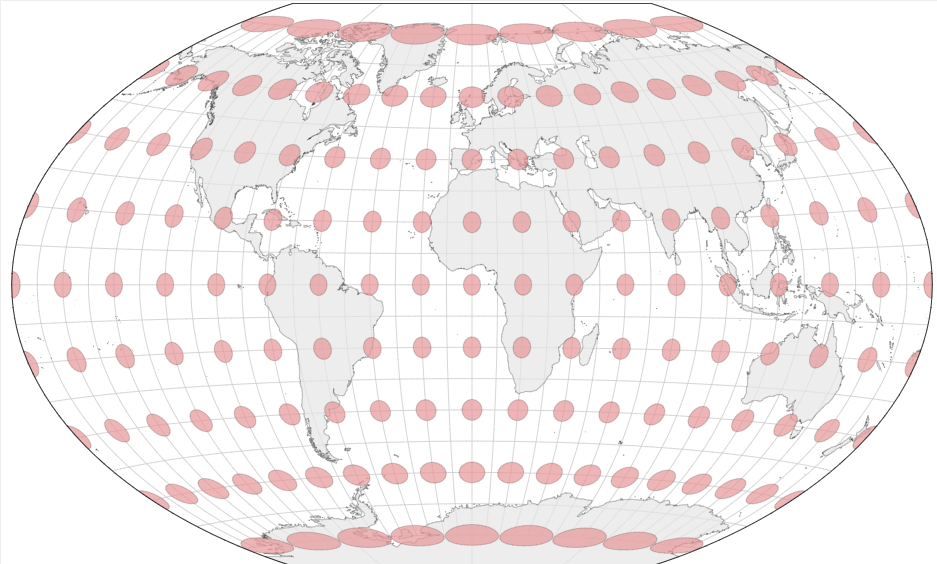
\includegraphics[width=0.3\linewidth]{img/comp} 

}

\caption{Ejemplo de proyección de compromiso: Winkel Tripel}\label{fig:comp}
\end{figure}

En los anteriores ejemplos se ha añadido a cada proyección la \textbf{indicatriz de
Tissot}. Ésta consiste en una serie de círculos imaginarios de igual área
distribuidos sobre la superficie esférica de la Tierra en determinados puntos.
De este manera, al presentar la indicatriz de Tissot en una proyección
específica, se puede entender de una manera intuitiva la distorsión provocada
por dicha proyección, ya que los círculos se ven distorsionados o preservados
según los parámetros y la naturaleza de la proyección en cuestión.

  \bibliography{book.bib}

\end{document}
